A detailed description of the SNO+ detector has been implemented in the RAT software package for Monte Carlo (MC) simulations, as mentioned in Chapter 3. However, when the simulations are compared to the real world, there always exist discrepancies. In order to make precise measurements, calibration sources were implemented in the SNO+ detector during the water phase and the partial-fill phase. During the water phase, the $^{16}$N source was used for the primary detector calibration. The $^{16}$N runs were mainly used for checking the performances of the reconstruction of the event position, direction and energy. The source was described in \ref{n16_description}.

In this chapter, I applied the MultiPath reconstruction algorithm mentioned in Chapter 4 to the $^{16}$N calibration data and simulations.

First, for the $^{16}$N calibration runs during the water phase, the MultiPath water (MPW) fitter was applied on both data and simulations. By comparing the differences between the data and MC, systematics of the position and direction reconstruction were extracted. Setting the MPW fitted event vertex and direction as seed, the event energy was reconstructed via the energy RSP fitter. Also based on the MPW fitted vertex and direction results, the other parameters, such as the in-time-ratio (ITR) and the isotropic parameter ($\beta_{14}$) were calculated. By comparing the $^{16}$N data and the MC simulations, the systematics were also evaluated. These systematic results were used in the solar neutrino analysis in Chapter 6.

The MultiPath water (MPW) fitter was also applied on the simulations of the AmBe source calibration runs during the water phase. The performances of the MPW fitter reconstruction on low energy events, specially the 2.2 MeV $\gamma$ events were discussed.

The last section of this chapter is to check the performance of the MultiPath partial fitter for the $^{16}$N calibration runs during the partial-fill phase. An attempt of extracting the Cherenkov signals from the events in the scintillator was made. This attempt will be useful for extracting the solar neutrino events and reconstructing their directions during the scintillator phase. 

\section{\isotope[16]{N} Calibration Scans in the Water Phase}\label{sect:n16_water}
During the water phase, the $^{16}$N calibration source was deployed as internal calibration scans in June and November, 2017 and as external scans in March, 2018. For each calibration run, the source was placed at a fixed position and the data were taken for about 20 minutes (for central run-107055, it took 1 hour). For the internal scans, the source was inside the AV, moving along x, y and z-axes (called ``X, Y, Z scans'' in this thesis). It was also was moved diagonally across the AV and was placed at the corners of the inner AV (``corner scans''). For the external scans, the source was placed in the external water region but outside the AV. The source was moved along z-axis with a fixed $(x,y)$ position close to the AV at (-5861.0,-2524.0)~mm. Fig.~\ref{N16_3Dscan} shows the different positions of the $^{16}$N source deployment. In this thesis, 79 internal scan runs and 19 external runs were used. Details of the calibration runs are listed in the tables in Appendix B. 

\begin{figure}[!htb]
	\centering
	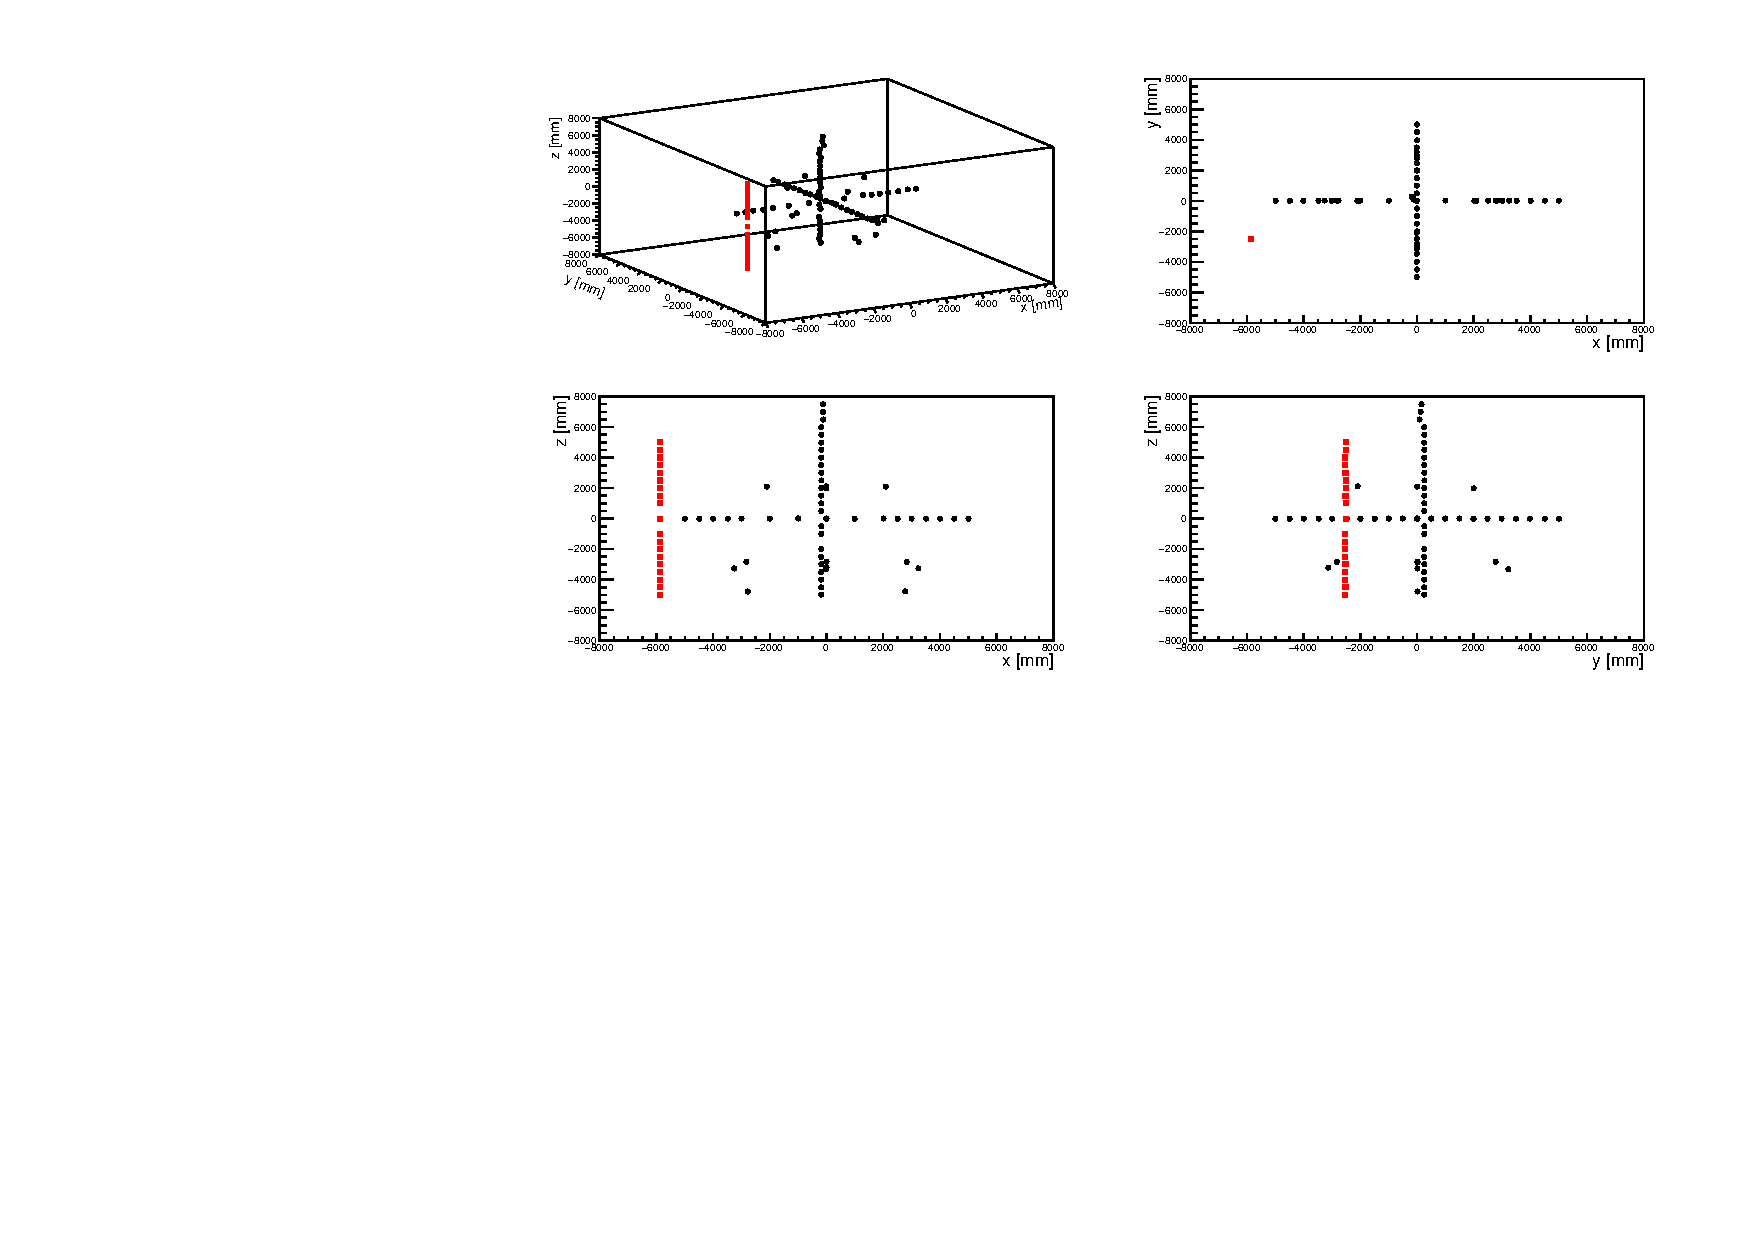
\includegraphics[width=15cm]{N16_3Dscan.pdf}
	\caption{The deployed source positions of the $^{16}$N scan runs used by this thesis. The black dots are internal runs while the red squares are external runs.}
	\label{N16_3Dscan}
\end{figure}

The $^{16}$N calibration runs provide ideal tests for the fitter performance. From a comparison of reconstructions for data and MC, we can also extract the resolution and bias of the fitter. Here I worked out the vertex and the direction reconstruction performances for both of the RAT water fitter and the MPW. The vertex shifts as well as the uncertainties were evaluated. 

To tackle with the $^{16}$N calibration data and simulations, an FECD tag cut ($FECD==9188$) was applied during the data processing to only save the events when the source trigger fired. A reconstruction threshold on $NHit$: $NHit>=6$ was used in both the MC and data. Besides these cuts, high level cuts based on classifiers were used. 

\section{High Level Cuts for the Water Phase}\label{sect:high_level_cuts}
A set of classifiers were developed by SNO analysis and been optimized for the SNO+ water analysis\cite{highlevel}. These classifiers utilized the reconstructed quantities, so valid reconstructions were always required.

\begin{itemize}
	\item[$\bullet$] In time ratio (ITR) classifier
	
	For each event, this classifier loops the triggered PMTs (hits), calculates the $t_{res}$ and then finds the ratio of the number of hits in an optimized prompt time window. In the water phase, the time window was [-2.5,5.0]~ns. If the ITR ratio is too low for an event, it indicates that most of the triggered PMTs are not caused by the prompt lights and thus the event probably does not originate from Cherenkov lights; it can be an instrumental nosse, or caused by a large amount of lights reflecting off the detector components (called ``late lights''). 
	
	\item[$\bullet$] $\beta_{14}$ isotropy classifier
	
	This classifier uses Legendre polynomials to return the	first ($\beta_1$) and the fourth ($\beta_4$) spherical harmonics of an event, where:
	\[
	\beta_l = \frac{2}{N(N-1)}\sum_{i=1}^{N-1}\sum_{j=i+1}^N P_l(\cos\theta_{ij})
	\]
	and $P_l(\cos\theta_{ij})$ are Legendre polynomials. 
	
	A combination of two $\beta_l$ terms was chosen by the SNO collaboration to be: $\beta_{14}=\beta_1+4\beta_4$. This quantity gives a gaussian-like distribution for Cherenkov events\cite{dunmore2004separation}.	In principle, any deviation from zero suggests some polarity or a deviation from a totally isotropic pattern.
	
	\item[$\bullet$] $\theta_{ij}$ isotropy classifier 
	
	This classifier describes the angle subtended at an event vertex by PMT \#i and PMT \#j, which is calculated as:
	\begin{equation}
	\cos\theta_{ij}=\frac{(\vec{X}_{PMT\#i}- \vec{X}_{event})\cdot (\vec{X}_{PMT\#j}- \vec{X}_{event})}{|\vec{X}_{PMT\#i}- \vec{X}_{event}||\vec{X}_{PMT\#j}- \vec{X}_{event}|}.
	\end{equation}
\end{itemize}

\subsection{Effects of the High-level Cuts}
As described above, the classifiers can help to distinguish the signals from Cherenkov events and backgrounds from non-Cherenkov events. To remove the non-Cherenkov backgrounds, cuts of $ITR>0.55$ and $-0.12<\beta_{14}<0.95$ (called ``high-level cuts'') were suggested by the collaboration\cite{waterunidoc}. These cuts are based on the analyses of data cleaning, simulated physics events as well as the SNO experience\cite{waterunidoc,marzec2019measurement,dunmore2004separation}.

The $^{16}$N central run-107055 data and MC were used to check the effects of the high-level cuts. For the MC (data), the cut of $ITR>0.55$ removed 0.69\% (0.79\%) of the total events; $-0.12<\beta_{14}<0.95$ removes 1.11\% (0.93\%) of the total events. Combining the ITR and $\beta_{14}$ cuts, 1.69\% (1.62\%) of the total events were removed.

The poorly reconstructed events with large position biases ($>6000~mm$) were counted.
For the MC case, the position biases were taken as the distance between the reconstructed positions and the true positions generated by the MC: $|\vec{X}_{fit}-\vec{X}_{MC}|$; while for the data case, the biases were between the reconstructed positions and the source manipulation position: $|\vec{X}_{fit}-\vec{X}_{src}|$. The large biases events are 0.13\% of the total events in both the MC and data. The high-level cuts removed 73.12\% (66.82\%) of them for the MC (data).

Fig.~\ref{n16_highLevelCut} shows the relations between the position biases and the $ITR$, $\beta_{14}$ respectively, for the data and MC.
\begin{figure}
	\centering
	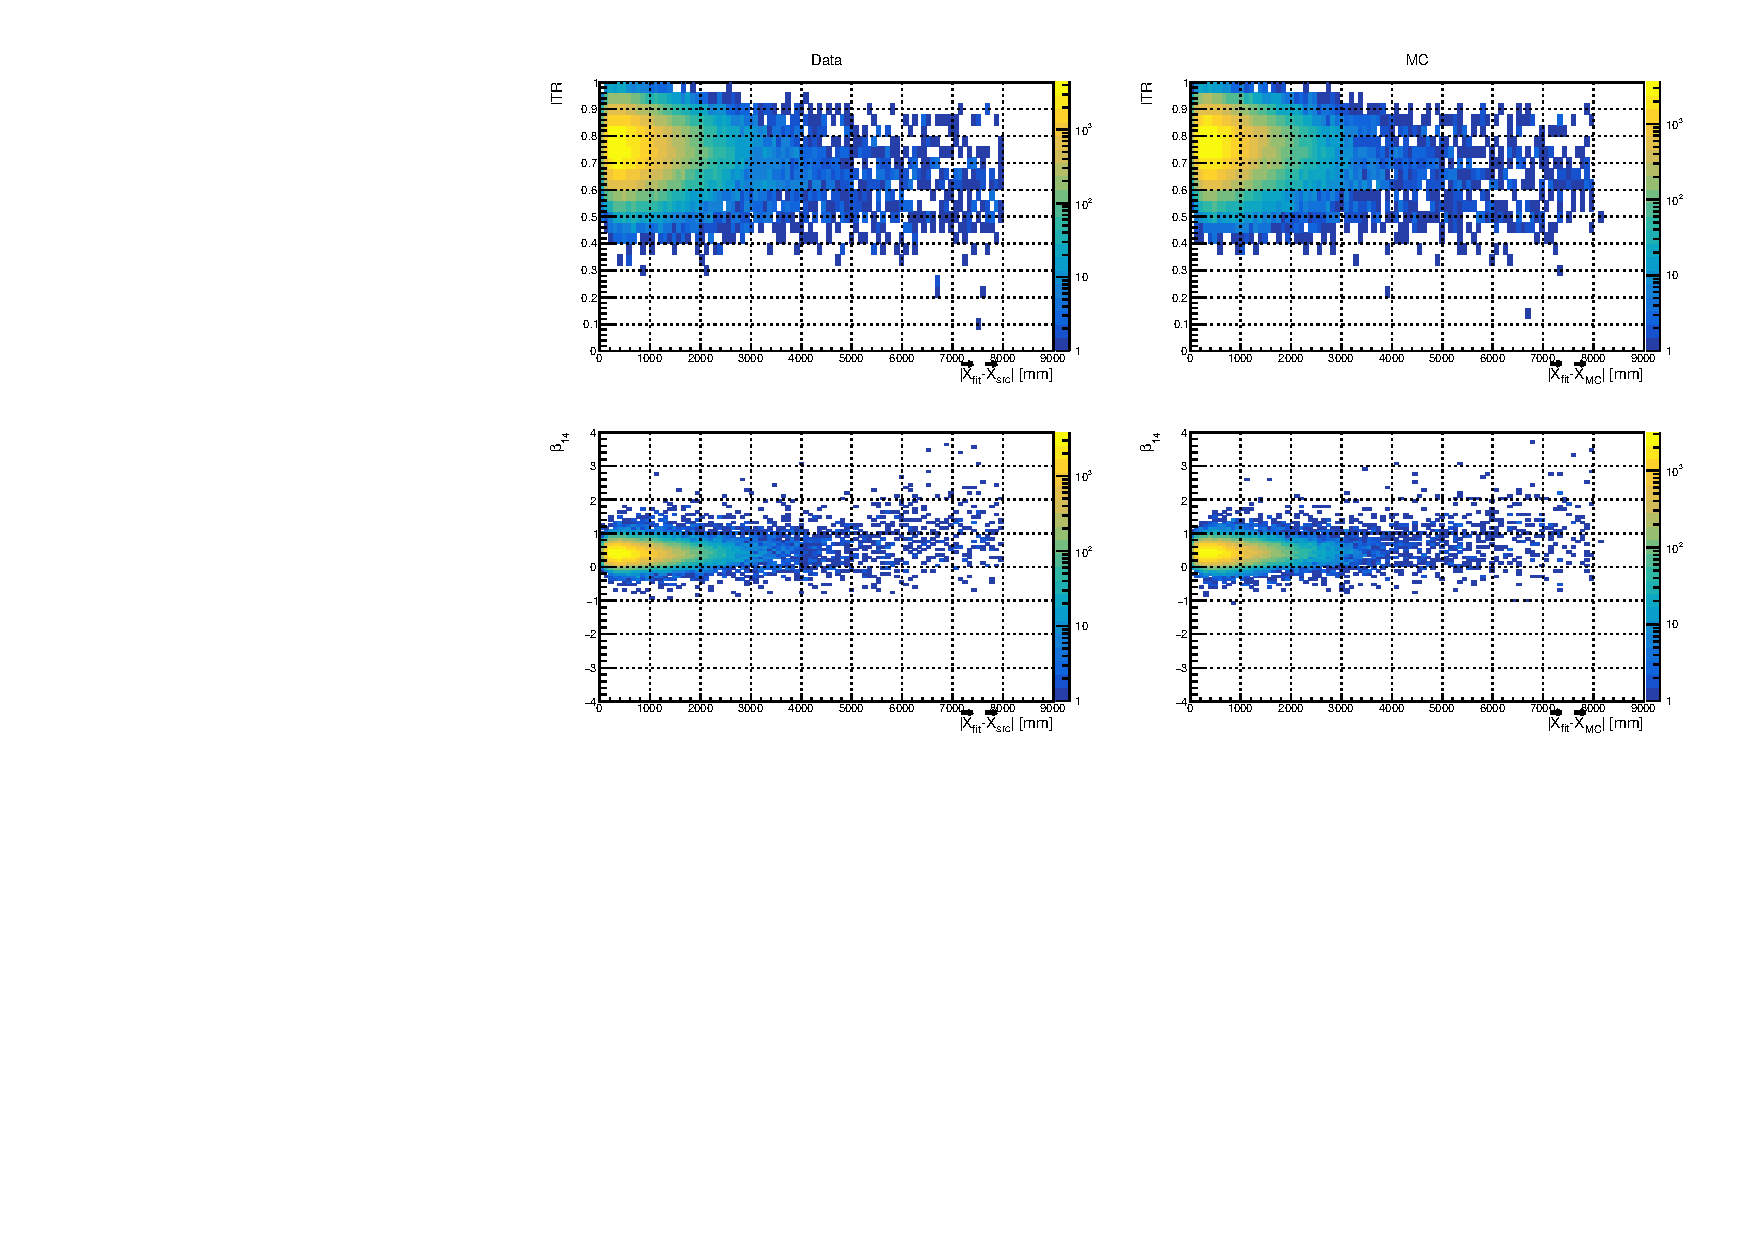
\includegraphics[width=14cm]{N16_107055_highLevelCuts.pdf}
	\caption{Position biases vs $ITR$ (top) and $\beta_{14}$ (bottom) for the $^{16}$N central run-107055. Left is MC and right is data. For the data, the source position ($\vec{X}_{src}$) was compared.}
	\label{n16_highLevelCut}
\end{figure}

As a summary, the high-level cuts removes more than a half of the events with large position biases while removes about 1.6\% of the total events. 

\section{Reconstruction Evaluations from $^{16}$N Calibration Scans in the Water Phase}

In this section, by analyzing the $^{16}$N data and MC in the water phase, I extracted the reconstruction resolutions of the event position, direction and energy respectively. Then by comparing the data with the MC, the reconstruction systematics were evaluated.

To do these evaluations, a few cuts were applied on both the data and MC. Firstly, the level cuts  ($ITR>0.55$, $-0.12<\beta_{14}<0.95$) were applied. For events with the position, direction and energy successfully reconstructed (i.e., the event has valid position, direction and energy reconstructions), further cuts on the reconstruction figure of merit (FoM) and source geometry (will be described in detail) were applied to ensure that the analyzed events were nicely reconstructed physics events caused by the source $\gamma$ particles interacting with the detector water.

\subsection{Position Reconstruction Evaluation}
\subsubsection{Position Figure of Merit}
A quantity called scaled logL ($scaleLogL$) is used as the position reconstruction FoM ($posFoM$): $scaleLogL = \ln L/NHit_{selected}$. This quantity utilizes the best log-likelihood returned by the MultiPath fitter for a successfully reconstructed event vertex, and then it is scaled by the ``selected'' $NHit$, i.e., the number of the PMTs actually used by the fitter for reconstructing the event vertex, after the PMT selections mentioned in \ref{sect:PMTselector}.

Fig.~\ref{posBiasVsFOM} shows the $scaleLogL$ with the position biases for the reconstructed events in $^{16}$N central calibration run-107055. Both of the data and the MC simulations are shown. For the MC case, the position biases are between the reconstructed positions and the true positions generated by the MC: $|\vec{X}_{fit}-\vec{X}_{MC}|$; while for the data case, the biases are between the reconstructed positions and the source manipulation position: $|\vec{X}_{fit}-\vec{X}_{src}|$.

\begin{figure}
	\centering
		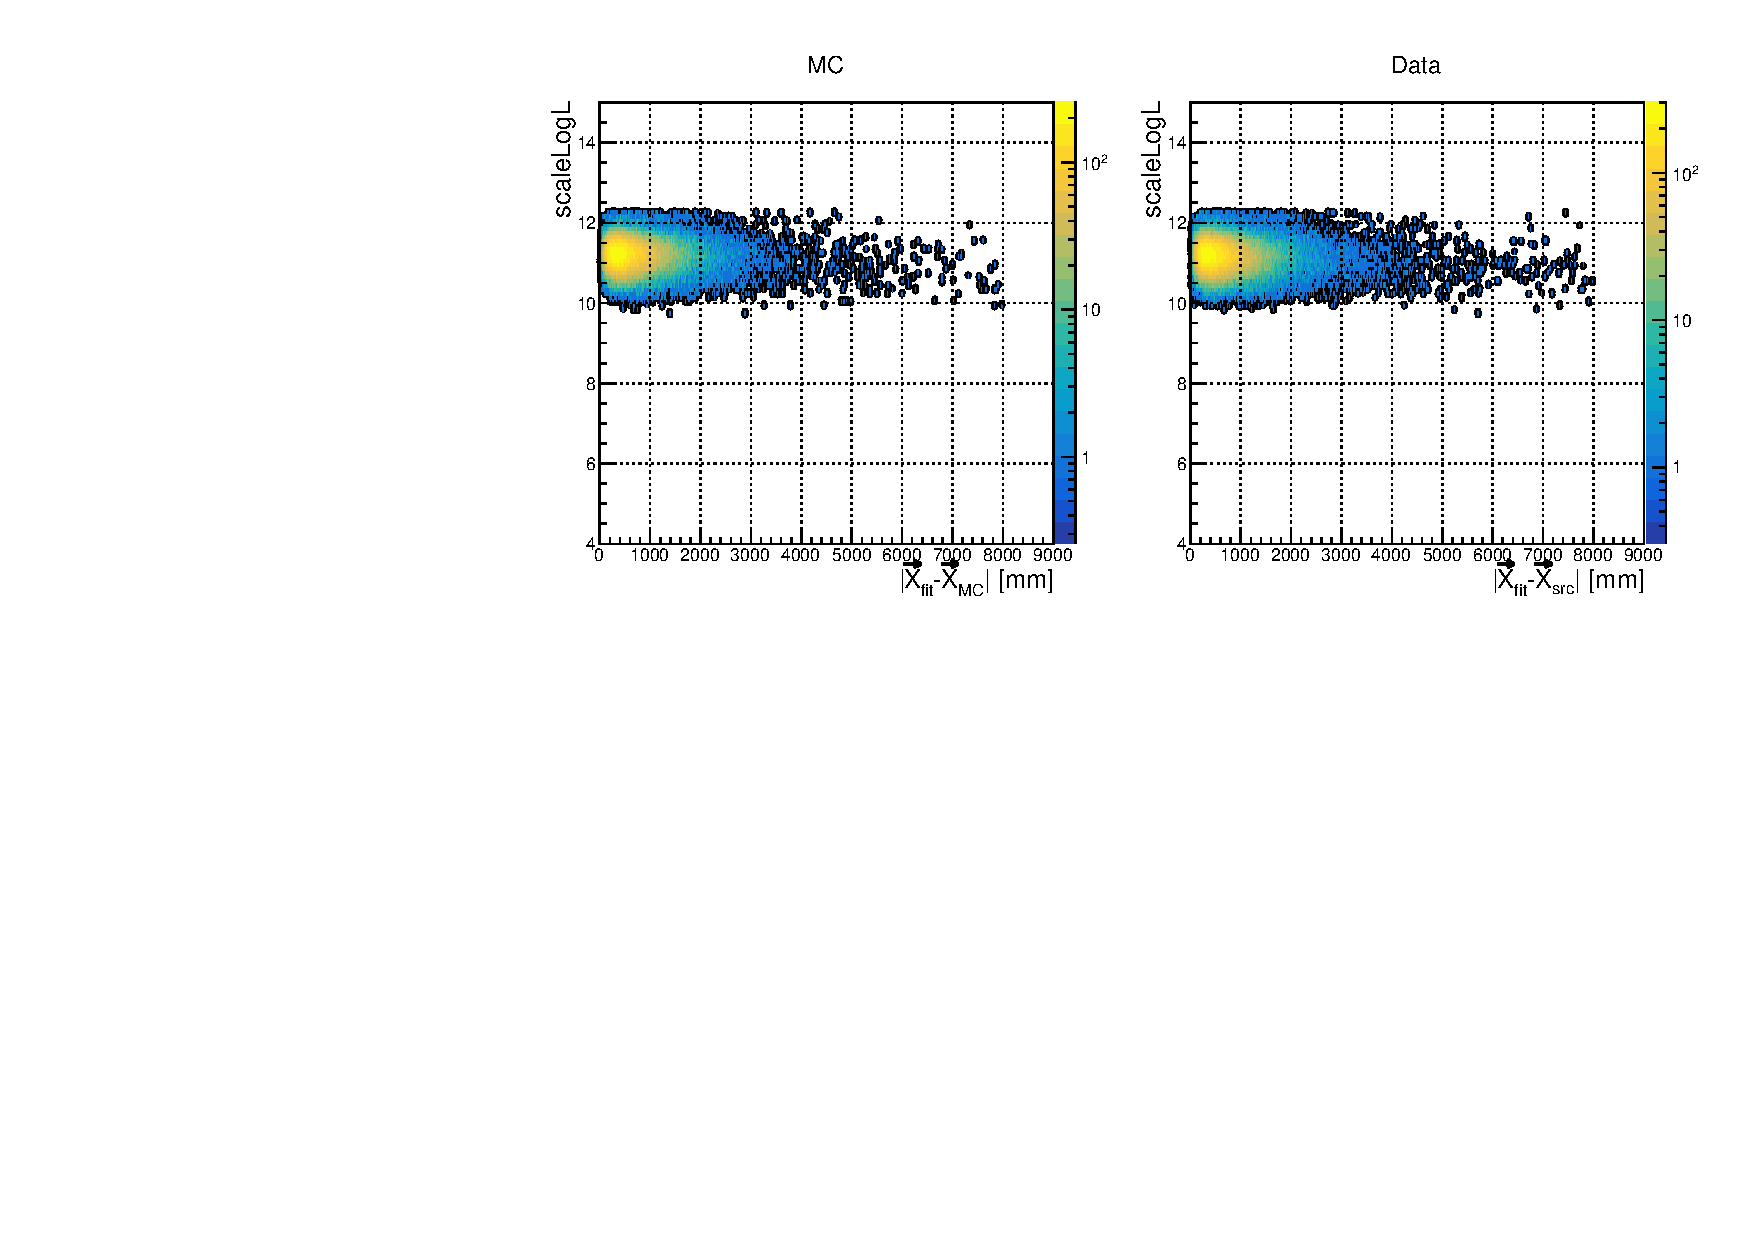
\includegraphics[width=13cm]{N16_107055_scaleLogLvsPosBias.pdf}
	\caption{Position biases ($|\vec{X}_{fit}-\vec{X}_{MC}|$) vs $scaleLogL$ for the $^{16}$N central run-107055. Left is MC and right is data. For the data, the source position ($\vec{X}_{src}$) was compared.}
	\label{posBiasVsFOM}
\end{figure}

For the MC (data) case, about 0.035\% (0.043\%) of the total reconstructed events have large biases ($|\vec{X}_{fit}-\vec{X}_{MC}|>6000~mm$). A cut of $scaleLogL>10$ removes 96.0\% (97.3\%) of the events which have biases over 6000 mm, with a sacrifice of removing 0.012\% (0.016\%) of the total events.

Fig.~\ref{energyVsFOM} shows a relation between the $scaleLogL$ and the reconstructed energy ($E_{fit}$). 

For the events with reconstructed energies below the water solar neutrino analysis threshold 3.5~MeV ($E_{fit}<3.5~MeV$), they are mostly coming from the $U/Th$ isotopes, decays of Potassium as well as instrumental noises\cite{waterunidoc}. Their lower energies or $NHits$ can affect the position reconstruction since there are fewer PMTs to be used and thus their $posFoM$ can be worse.
In the MC (data) case, there are about 13.04 \% (12.89\%) of the events with $E_{fit}<3.5~MeV$. By applying the cut of $scaleLogL>10$, 0.10\% (0.09\%) of such events were removed.

\begin{figure}[!htb]
	\centering
	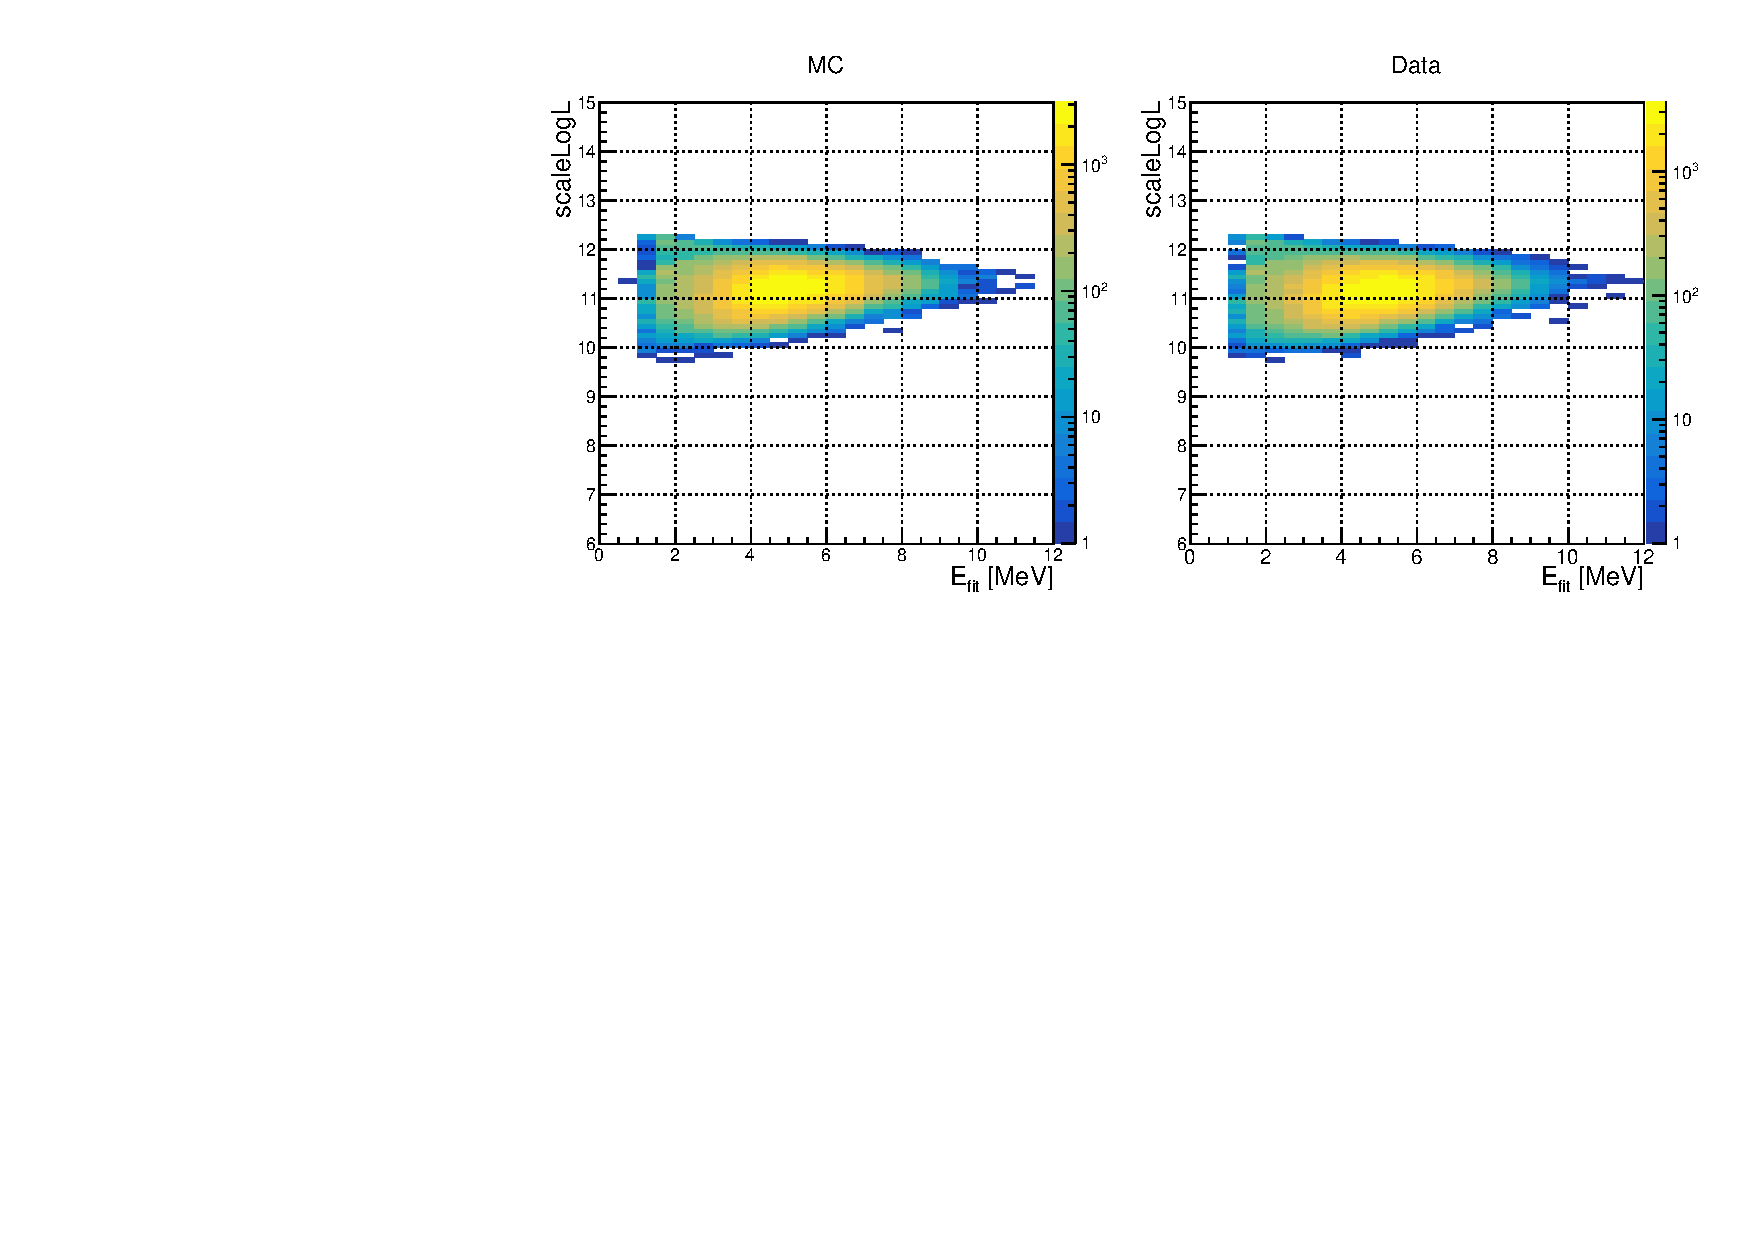
\includegraphics[width=13cm]{N16_107055_scaleLogLvsEnergy.pdf}
	\caption{Reconstructed energy vs $scaleLogL$ for the $^{16}$N central run-107055. Left is MC and right is data.}
	\label{energyVsFOM}
\end{figure}

As a summary, there are about 0.04\% of the reconstructed events which were poorly reconstructed (mis-reconstructed) by the MPW fitter with position biases over 6 meters. Applying a cut in $posFoM$ with $scaleLogL>10$ can remove over 96\% mis-reconstructed events. This $posFoM$ cut was used in the following direction and energy reconstruction evaluations.

\subsubsection{Position Resolution}
A position resolution function is defined for the reconstructed electron position distribution\cite{boulay2004direct}:
\begin{equation}
R(x)=\frac{1-\alpha_e}{\sqrt{2\pi}\sigma_p}\exp{[-\frac{1}{2}(\frac{x-\mu_p}{\sigma_p})^2]+\frac{\alpha_e}{2\tau_p}\exp{[\frac{-|x-\mu_p|}{\tau_p}]}},
\end{equation}
where $\alpha_e$ is the fractional exponential component, $\sigma_p$ is
the Gaussian width (corresponding to the position resolution), $\mu_p$ is the Gaussian shift (corresponding to the position bias) and $\tau_p$ is the exponential slope (corresponding to the position distributions in tails).

The $\gamma$-rays emitted from the $^{16}$N source interact with the water in the detector mainly via Compton scattering, as shown in Fig.~\ref{N16centralDiagram}. The position distribution of the $\gamma$ interaction vertices is peaked around the source container, spreading to about 2 meters.

\begin{figure}[!htb]
	\centering
	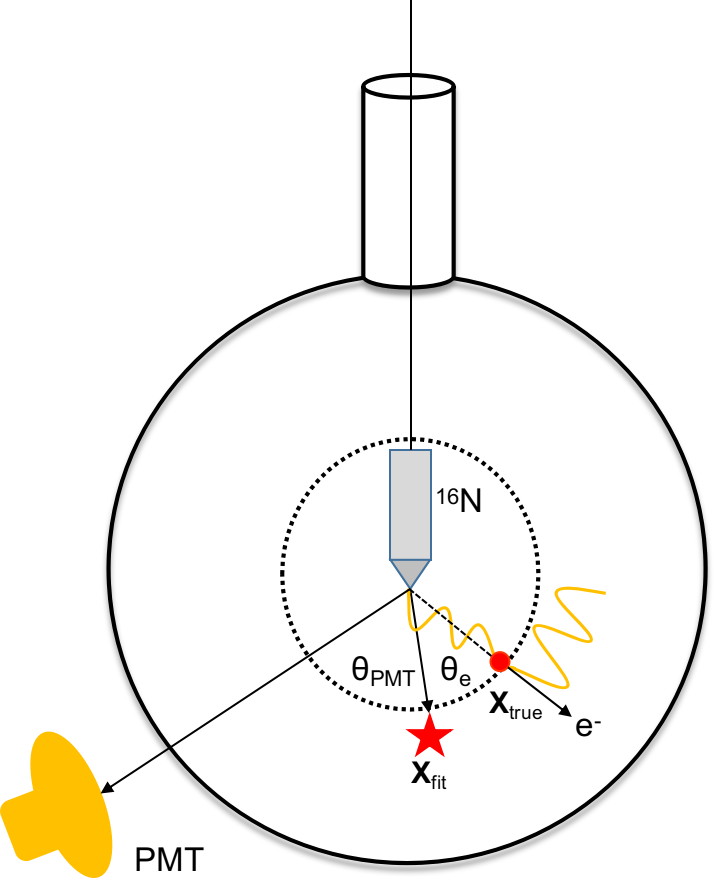
\includegraphics[width=8cm]{N16centralDiagram.png}
	\caption{A cartoon shows the $^{16}$N source.}
	\label{N16centralDiagram}
\end{figure}

Fig.~\ref{hsx} shows the spatial distributions $S(x)$ of the first $\gamma$-ray interaction positions projected on the x axis obtained from MC simulation. Therefore, the $^{16}$N source is considered as an electron source with a known spatial distribution\cite{boulay2004direct}. For simplicity, in the following we always discuss the $x$ component of the position vector $\vec{X}$. 

\begin{figure}[!htb]
	\centering
	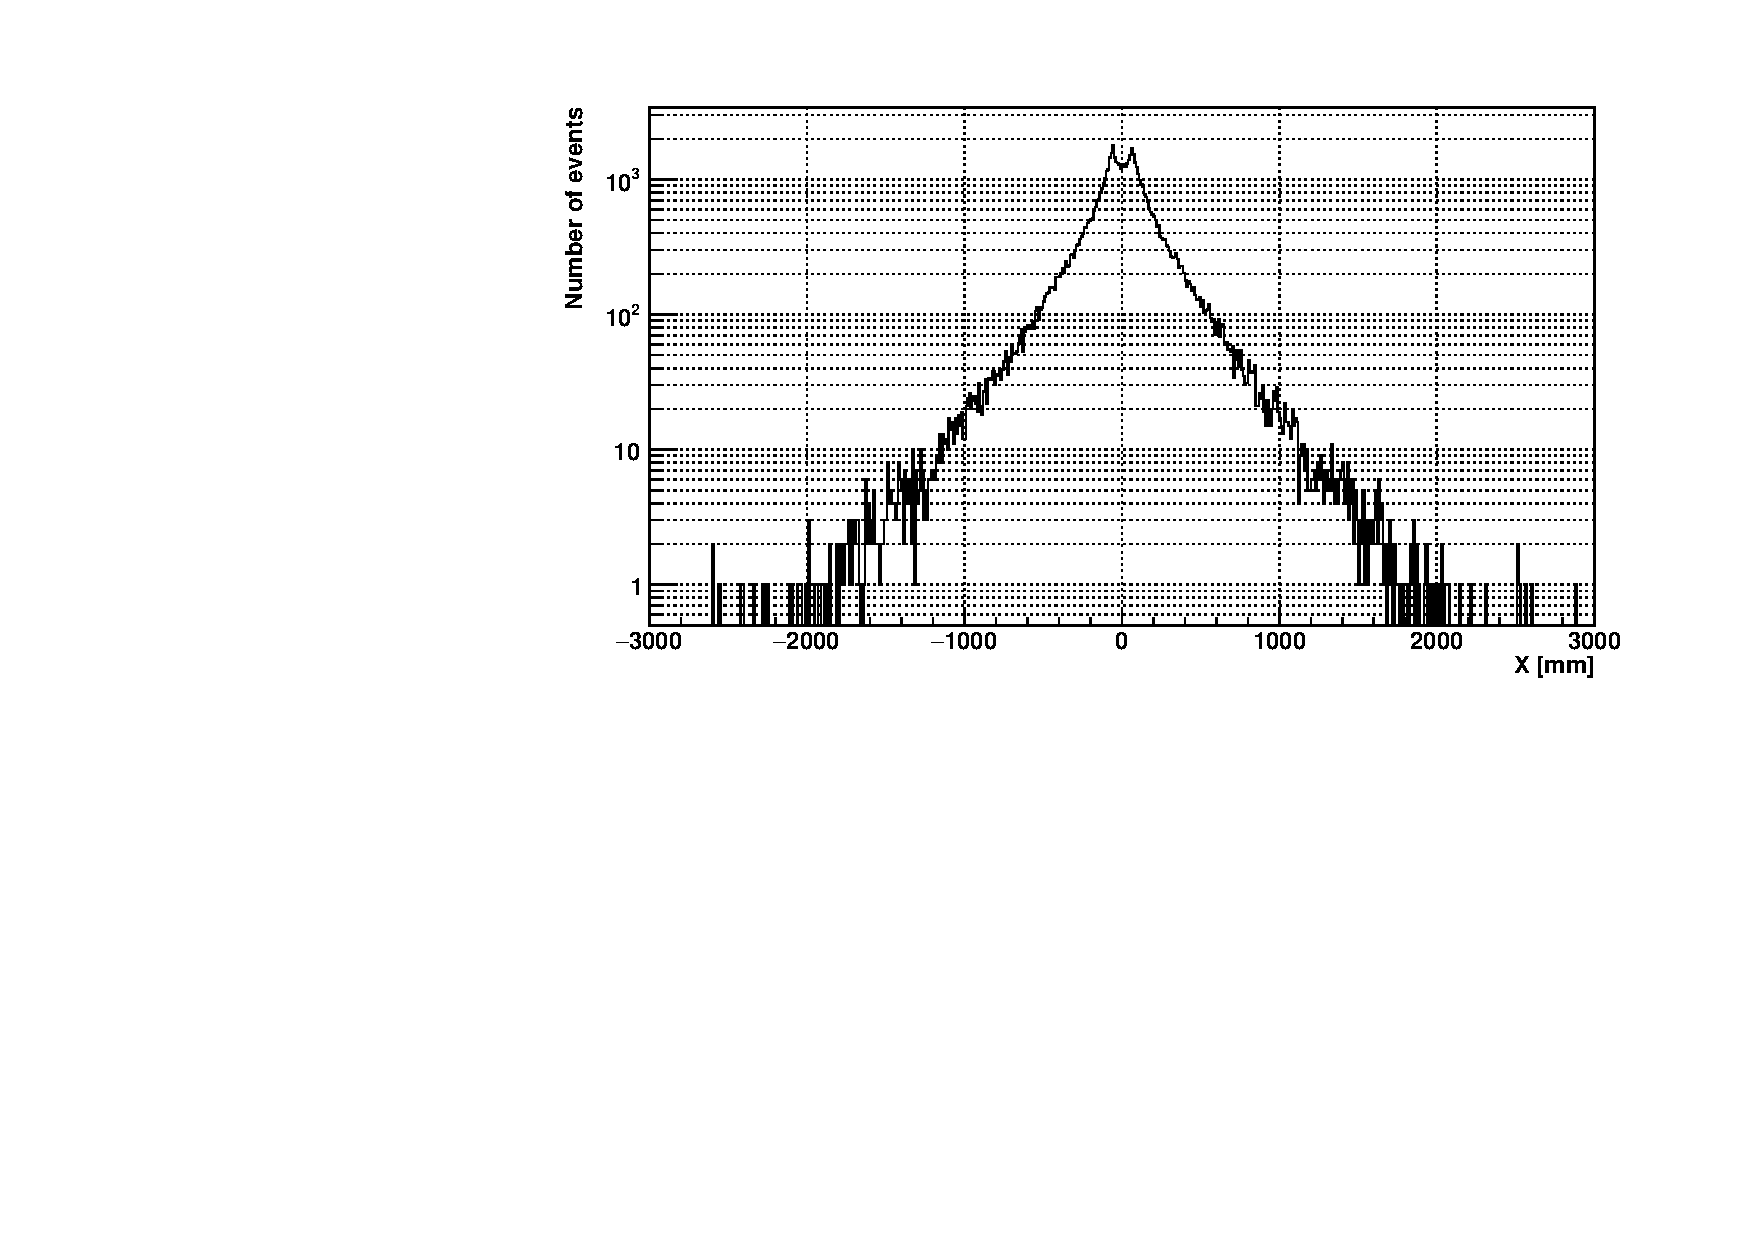
\includegraphics[width=12cm]{sx.pdf}
	\caption{Spatial distributions of {$^{16}$}N first $\gamma$-rays interaction position projected on x axis, obtained from the RAT simulations. The double-peak structure is due to the wall of the stainless steel container of the $^{16}$N source.}
	\label{hsx}
\end{figure}

For electrons from the $^{16}$N calibration source, their spatial distribution function $N_{R}(x)$ can be described by the position resolution function smeared by the convolution of $S(x)$ as\cite{boulay2004direct}:
\[
N_{R}(x)=\int^{+\infty}_{-\infty} S(x)R(x_{fit}-x)dx.
\]

The values of $N_{R}(x)$ can be calculated bin by bin from the histograms of $S(x)$ and $R(x)$ extracted from the MC or data: 
\[
N_R(x_i)=\sum_{x_i=-\infty}^{+\infty}S(x_i)R(x_{fit}^i-x_i).
\].

The $\chi^2$ is calculated by:
\[
\chi^2=\sum^{N_{bins}}_{i=0}[\frac{N_R(x_{fit}^i)-N_R^{fit}(x_{fit}^i)}{\sigma_i}]^2,
\]
where $N_R^{fit}$ is a trial fit to the $N_R$ by tuning the $\{\alpha_e,\mu_p,\sigma_p,\tau_p\}$ and $\sigma_i$ is taken as the bin width of the histograms.

By minimizing the $\chi^2$, the parameters of the resolution function, $\{\alpha_e,\mu_p,\sigma_p,\tau_p\}$ and a best $N_R^{fit}$ were obtained.

Fig.~\ref{fig:posresol} shows a comparison of the reconstructed x position of {$^{16}$}N events between data and MC. The reconstructed position distributions were fitted with $N_R^{fit}$.

\begin{figure}
	\centering
	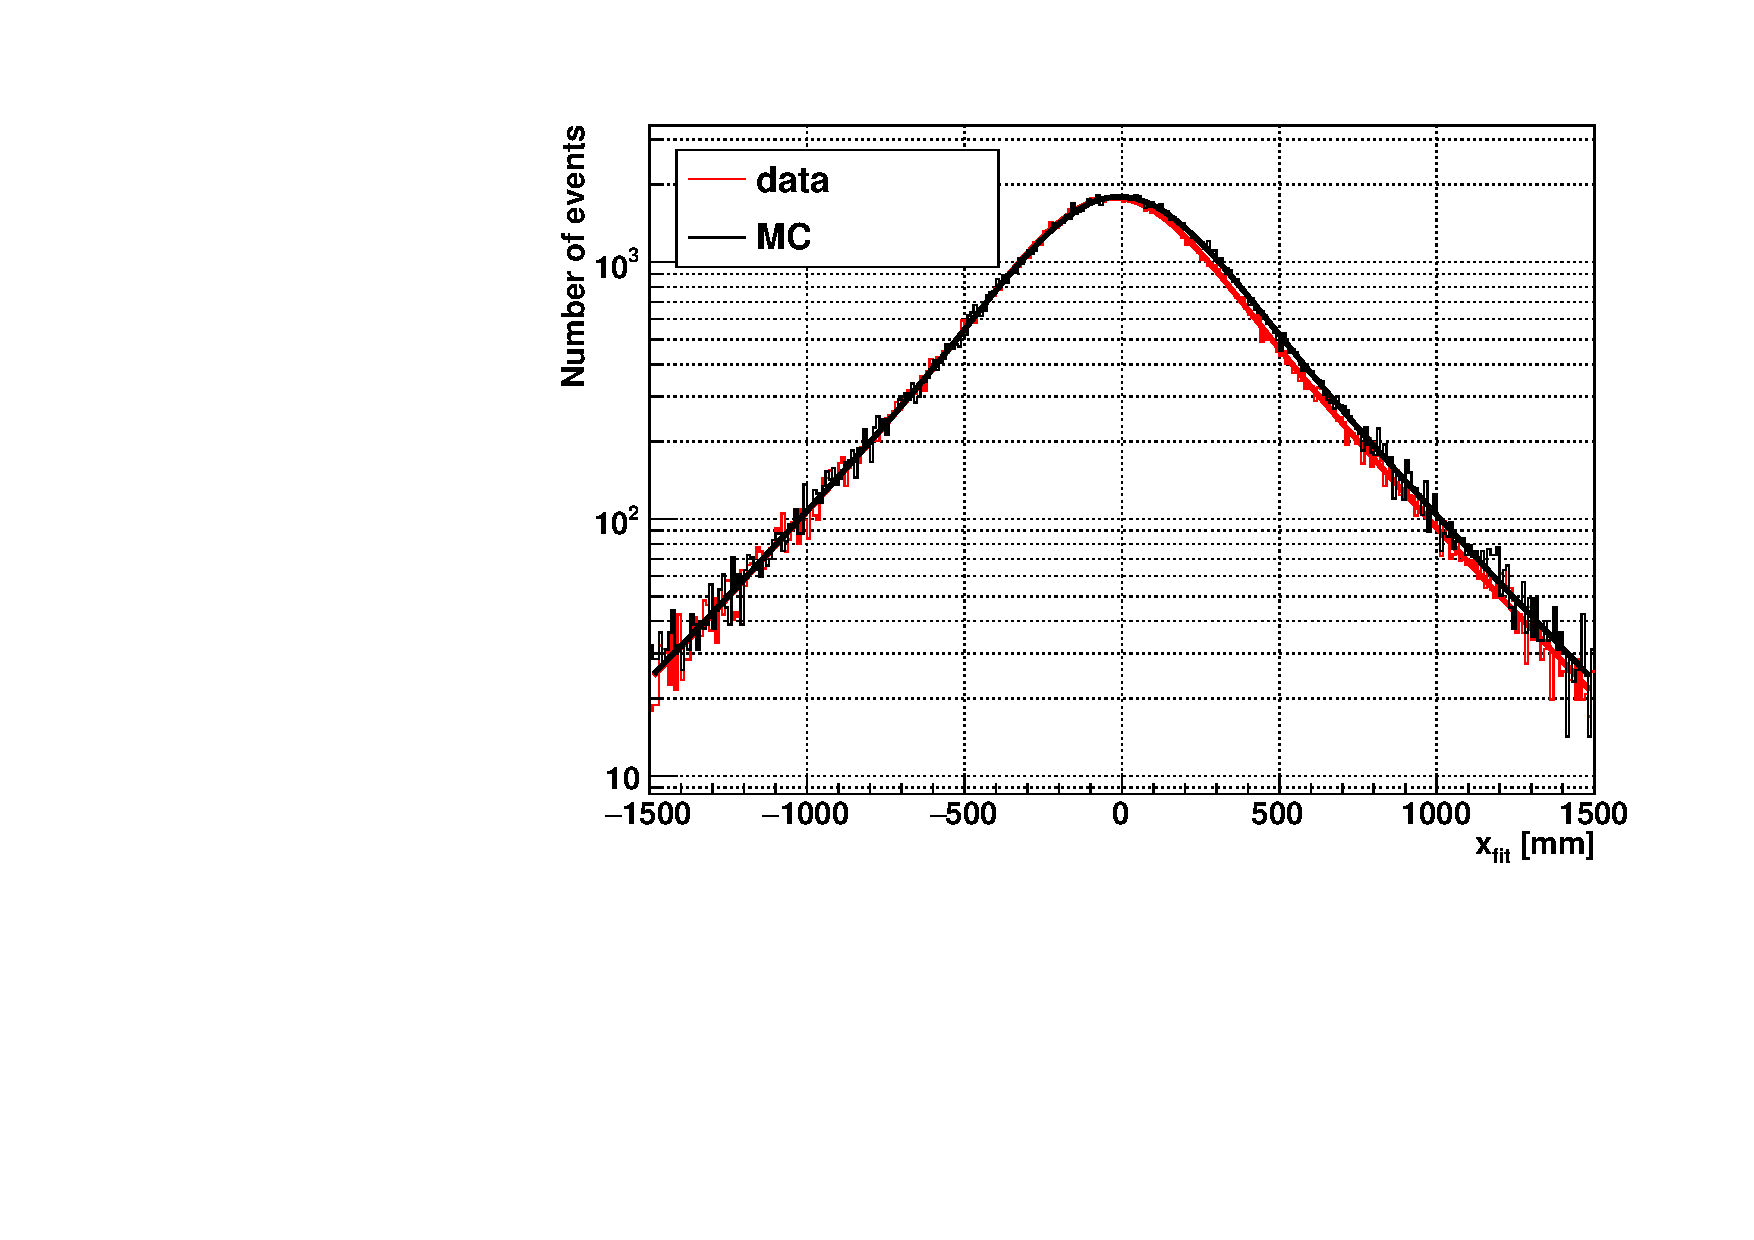
\includegraphics[width=140mm]{posResol.pdf}
	\caption{Distributions of the reconstructed position projected on x axis, obtained from SNO+ {$^{16}$}N central run data (red) and MC (black). The distributions are fitted with $N_R^{fit}$ (red and black lines).}
	\label{fig:posresol}
\end{figure}

Table~\ref{table_posresol} summarizes the values of position resolution parameters (for x-axis) obtained from data and MC of {$^{16}$}N calibration runs at the detector center.
\vspace{1mm}
\begin{table}[ht]
	\centering
	\caption{Position resolution parameters for the MPW fitter (x-axis).}
	\label{table_posresol}
	\begin{tabular}{ccccc}
		\toprule
		MPW fitter & $\alpha_e$ & $\sigma_P$ (mm) &  $\tau_P$ (mm)& $\mu_P$ (mm)\\
		\hline 
		data& 0.58$\pm$0.04 & 175.8$\pm$3.8 & 288.0$\pm$5.7 & -28.8$\pm$1.0\\	
		\hline 
		MC & 0.51$\pm$0.05 & 195.2$\pm$3.3 & 298.4$\pm$6.1 & -10.9$\pm$1.0\\
		\bottomrule
	\end{tabular}
\end{table}
\vspace{1mm}

\subsubsection{Position Systematics}
To evaluate the position uncertainties, the MC and data runs of the $^{16}$N internal scans along x, y, z axes were taken to evaluate the x, y, z position uncertainties respectively (the runs are listed in Table.~\ref{table:n16scanTable_zscan} to ~\ref{table:n16scanTable_xscan}. Three neck runs in z-scan were not used). The high-level cuts as well as the $E_{fit}>3.5~MeV$ and $scaleLogL>10$ cuts were applied. 
fit range was set as $[-2000, +2000]~mm$. If the lower range was smaller than -6000~mm, it was set to -6000~mm; if the upper range was larger than 6000~mm, it was set to +6000~mm. This was used to remove the effects caused by the AV.

The position resolution function was first fitted with 4 free parameters: $\alpha_e,\mu_p$, $\sigma_p$ and $\tau_p$. The the average values of the $\alpha_e$
and $\tau_p$ were calculated from all the scan runs used here. To simplify the calculation in propagating systematics, the $\alpha_e$ and the $\tau_p$ were fixed to the average value: $\alpha_e=0.5288$ (0.5375) for the MC (data); $\tau_p=271.738$ (263.735) for the MC (data). With the fixed values of $\alpha_e$ and $\tau_p$, both the data and the MC were refit with $\mu_p$ and $\sigma_p$ only. Using the fixed values of $\alpha_e$ and the $\tau_p$ is based on the reasons that these parameters in principle can be viewed as corrections to the $\gamma$ distribution ($S(x)$) and they can be absorbed, which would not depend on position\cite{waterunidoc}. 

Fig.~\ref{MPWscanXYZResols} shows the fitted results of $\mu_P$ and $\sigma_P$ along the x, y, z-axes scans respective. For the sake of simplicity, for the x-scan case, only the x-axis results ($\mu_{P,x},\sigma_{P,x}$) are shown here. Similarly, only the $\mu_{P,y}$ and $\sigma_{P,y}$ ($\mu_{P,z}$ and $\sigma_{P,z}$) are shown for the y-scan (z-scan). The relative differences discussed later consider all the three-axes.

\begin{figure}
	\centering
	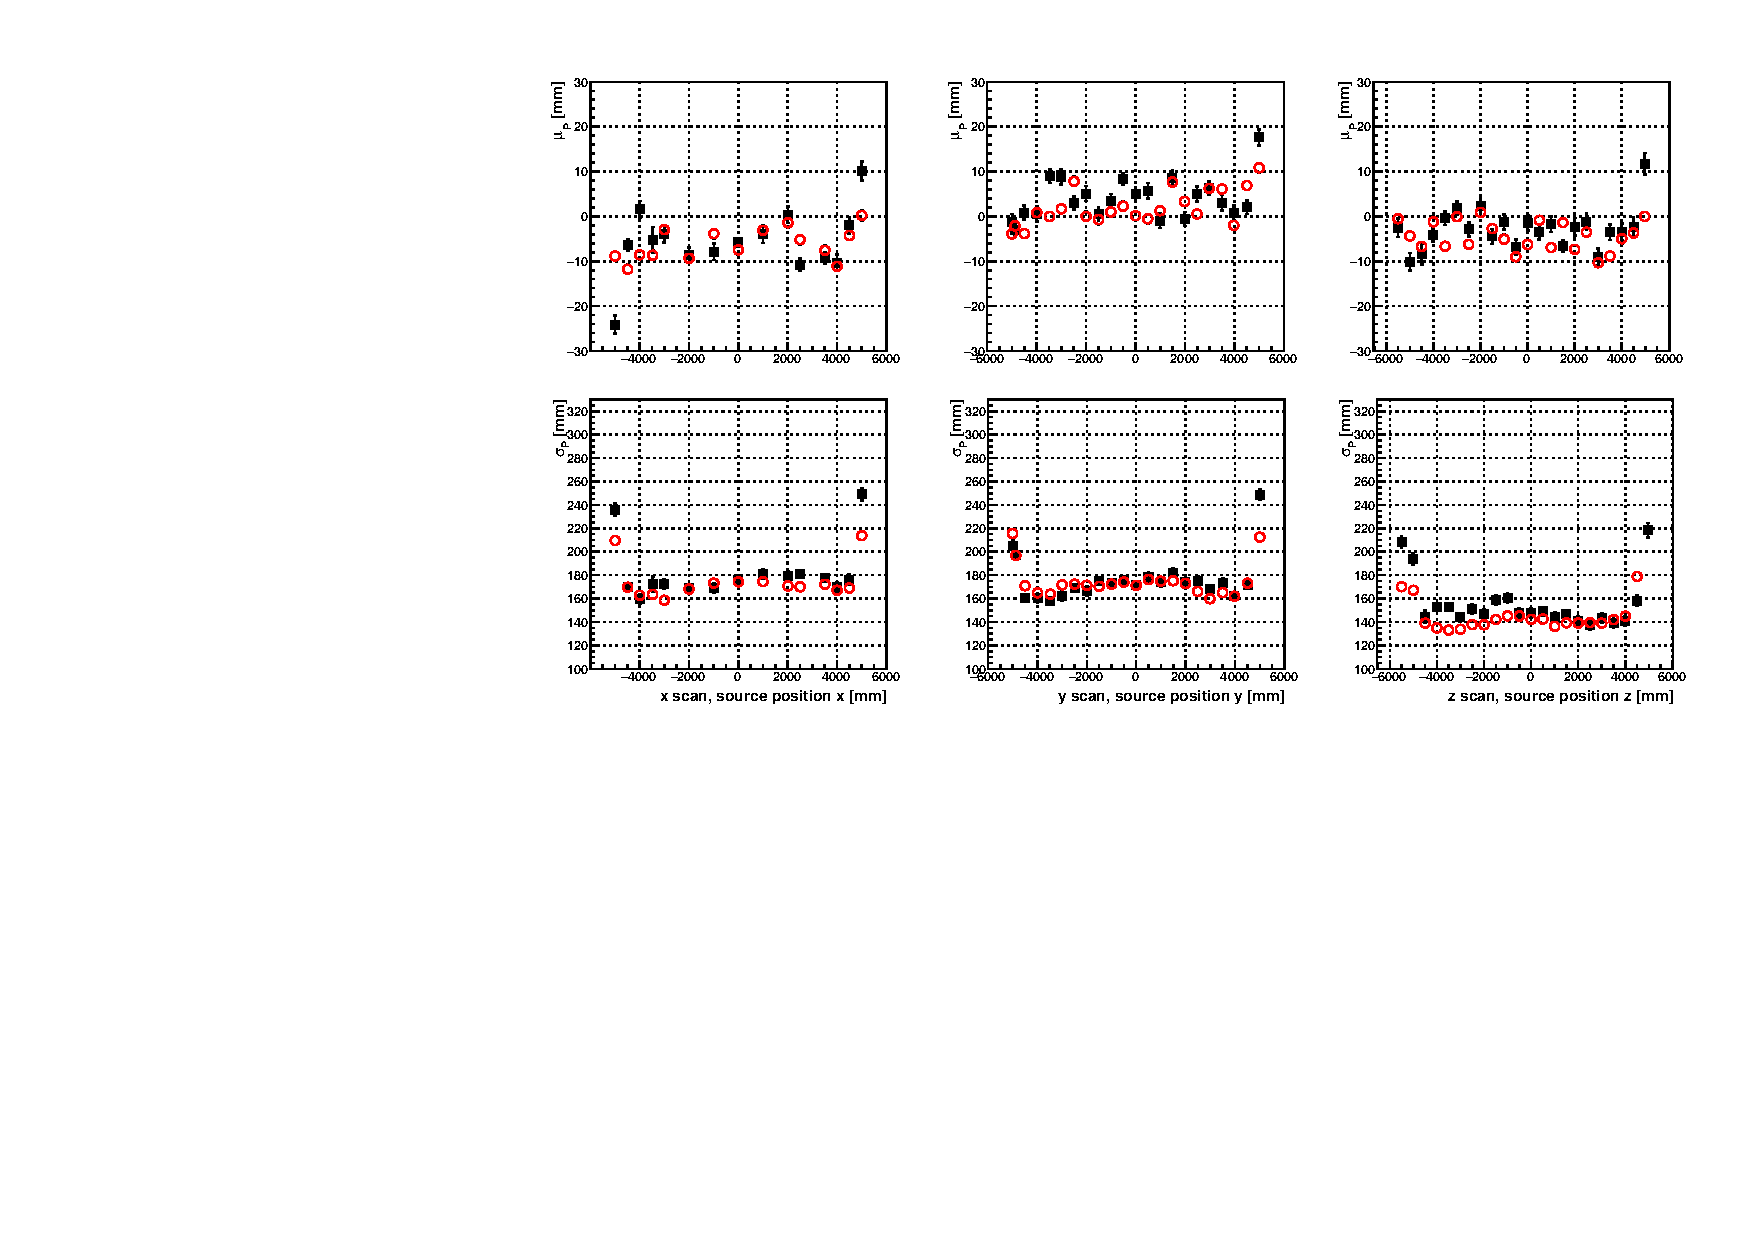
\includegraphics[width=16cm]{N16_rat6176_muPandSigmaP_xyzScans.pdf}
	\caption{The fitted values of $\mu_P$ (top three) and $\sigma_P$ (bottom three) along x (left), y (middle) and z (right) scans. The MC results (red circles) are compared with the data (black boxes).}
	\label{MPWscanXYZResols}
\end{figure}

It shows that the position resolutions of the MC are mostly better than the data, which is expected since the non-uniformities of the detector in realistic situation can cause a broader resolution in the data\cite{waterunidoc}. Also, when the source is close to the AV or at the edges of the axes, the Gaussian shift $\mu_P$ becomes large and the resolution goes worse. Also, the difference between the MC and data becomes large.

To quantify the discrepancies between the MC and data, a relative difference of $\sigma_p$ between the MC and data is defined as\cite{waterunidoc}:
\begin{equation}
\sigma_{p,\delta}\equiv\sqrt{\sum_i|(\sigma^{data}_{P,i})^2-(\sigma^{MC}_{P,i})^2|}~~(i=x,y,z),
\end{equation}
 
Fig.~\ref{pos_relative_sigma_biasesVsPositions} shows the $\sigma_{p,\delta}$ changing along the internal x, y and z-axes scans respectively. All the differences are below $190~mm$ except the run-106979 with the source at $z=4973.567~mm$. This worst resolution can be caused by the neck effects. 

It goes worse when the source is close to the AV or at the edges of the axes. When the source is close to the AV center, the differences are below $100~mm$.

\begin{figure}[!htb]
	\centering
	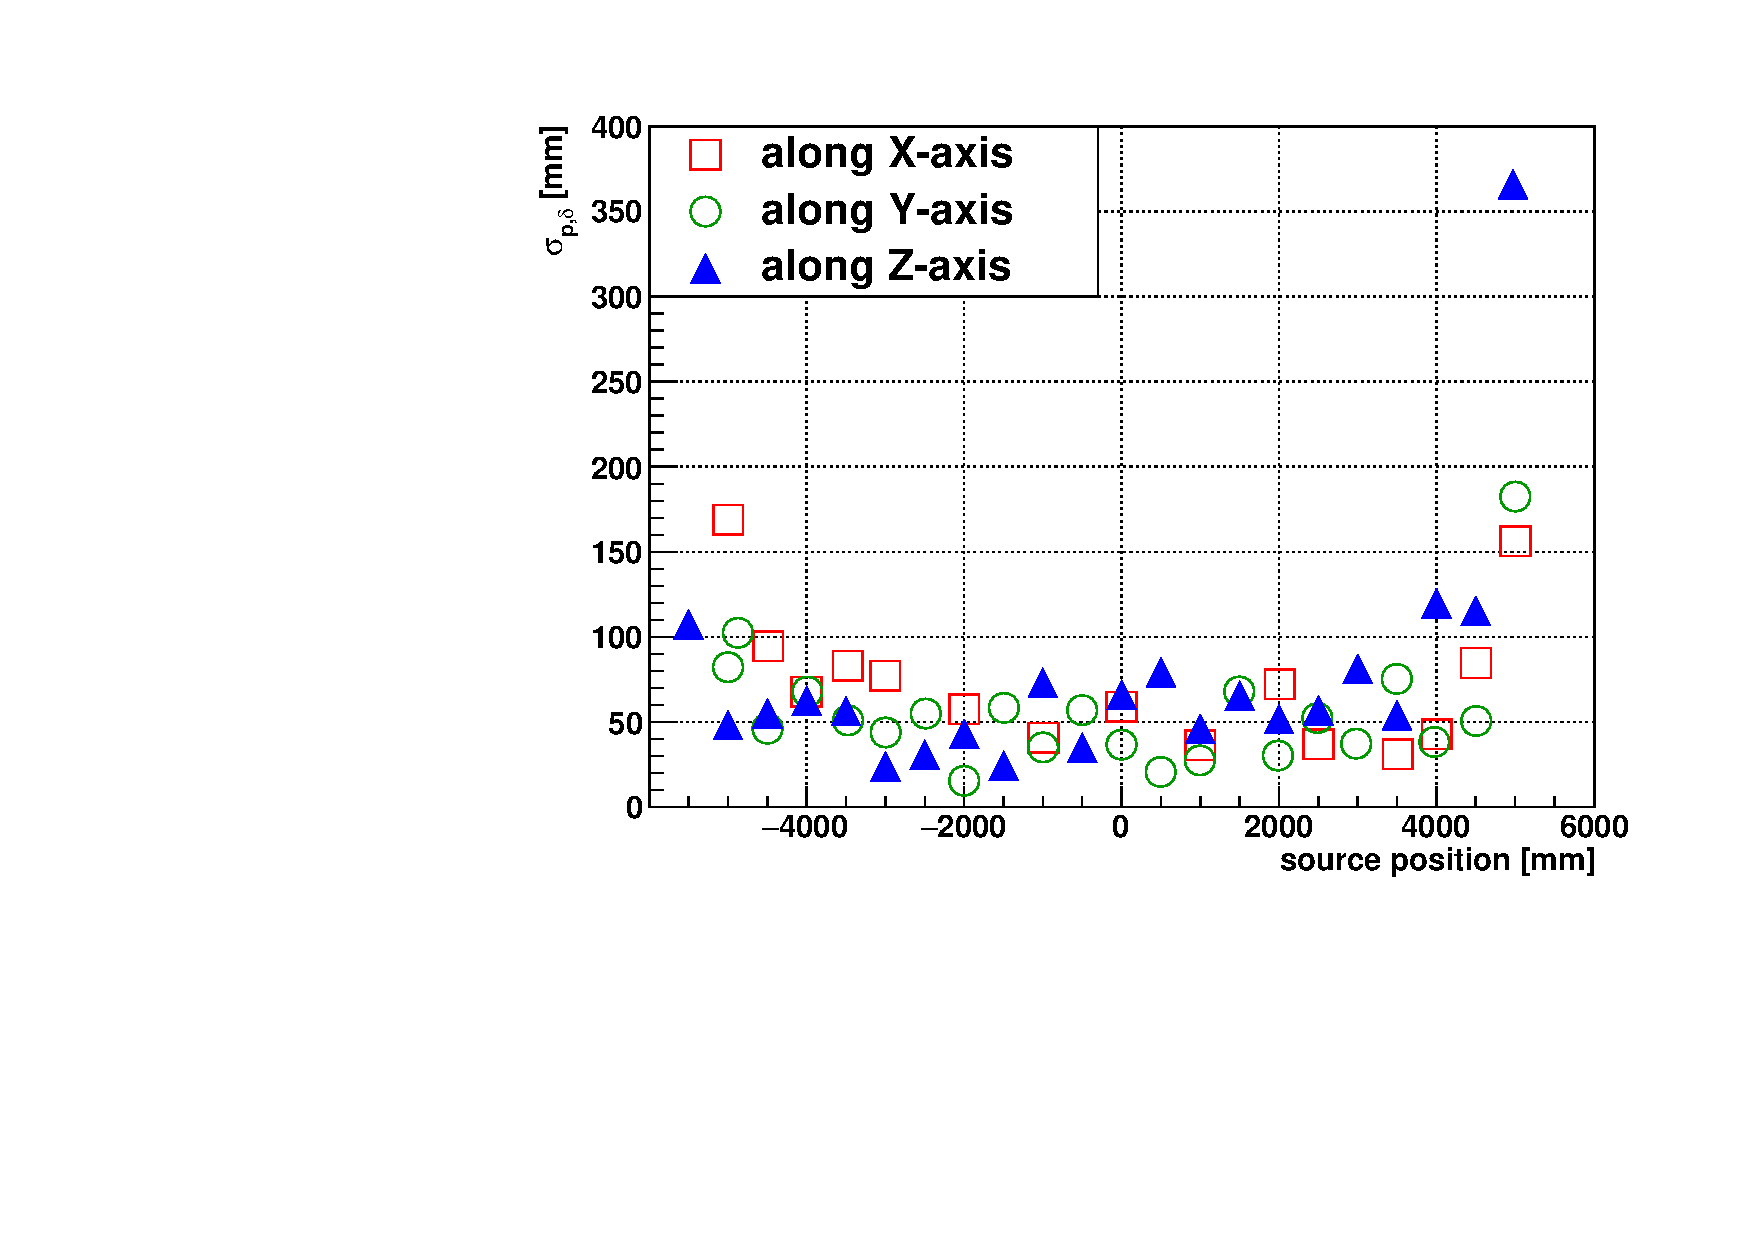
\includegraphics[width=16cm]{N16_6176_pos_sigmaP_data_mc.pdf}
	\caption{Relative differences of $\sigma_P$ ($\sigma_{p,\delta}$) as a function of the $^{16}$N source position. For simplicity, the corner scans are not shown in this figure. The red squares represent the results from the x-scan runs; green circles represent the y-scan runs and the blue triangles represent the z-scan runs.}
	\label{pos_relative_sigma_biasesVsPositions}
\end{figure}

The values of $\sigma_{p,\delta}$ were taken to represent the position resolution systematics.

In Table.~\ref{vertexResolsSystem}, the averages and the standard deviations were taken as the resolution systematics for x, y and z-axes respectively. To smear the position results, a Gaussian distribution $\mathcal{N}(0,\delta)$ was convolved with positions. The upper values $\delta$ were used to smear the positions.
\begin{table}[ht]
	\centering
	\caption{The MPW fitter position resolution systematic uncertainties in x, y and z axes. Unit: mm.}
	\vspace{3mm}
	\label{vertexResolsSystem}
	\begin{tabular*}{140mm}{c@{\extracolsep{\fill}}ccc}
		\toprule
		axis & systematic uncertainties & systematic to be applied ($\delta$) &smearing\\
		\hline 
		x  & $73.89\pm39.71$ & 113.6 & $x+\mathcal{N}(0,\delta)$\\
		y  &  $53.82\pm33.40$ & 87.22 & $y+\mathcal{N}(0,\delta)$\\
		z   & $76.45\pm65.54$ & 141.99 & $z+\mathcal{N}(0,\delta)$\\
		\bottomrule
	\end{tabular*}
\end{table}

To quantify the vertex shifts between the MC and data, values of vertex shifts: $\mu_P(data)-\mu_P(MC)$ were calculated for the x, y and z scans respectively. Fig.~\ref{fig:verteshitfs} shows these results.
\begin{figure}[!htb]
	\centering
	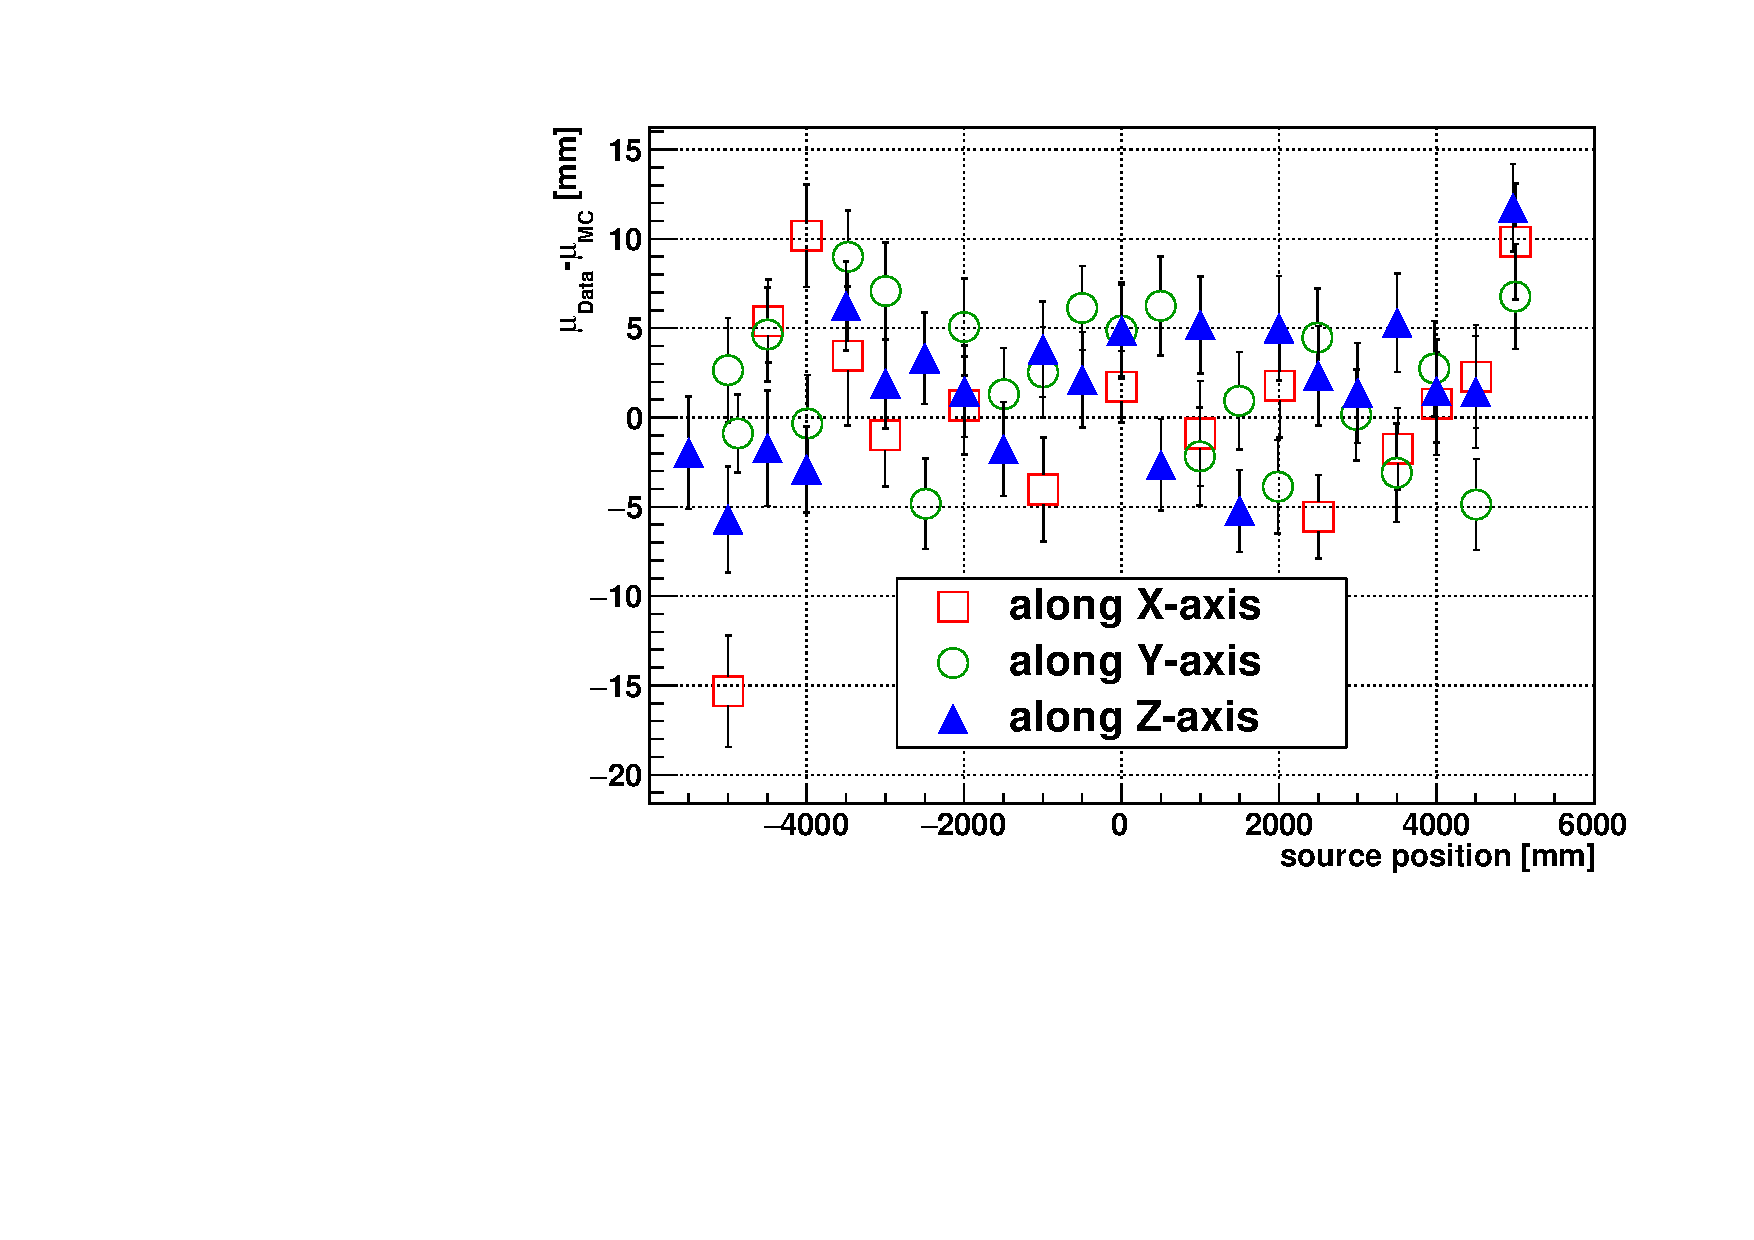
\includegraphics[width=16cm]{N16_rat6176_vertexShift_xyzScans.pdf}
	\caption{Vertex shifts of $\mu_P$ ($\mu_{p,\delta}$) as a function of the $^{16}$N source position. For simplicity, the corner scans are not shown in this figure. The red squares represent the results from the x-scan runs; green circles represent the y-scan runs and the blue triangles represent the z-scan runs.}
	\label{fig:verteshitfs}
\end{figure}

In Table.~\ref{vertexShifts}, the averages and the standard deviations were taken as the vertex shifts for x, y and z-axes respectively. To smear the position results, the positions were simply shifted by the upper values $\delta$ were used to smear the positions.
\begin{table}[ht]
	\centering
	\caption{Vertex shifts for the reconstructed positions in x, y and z axes. Unit: mm.}
	\vspace{3mm}
	\label{vertexShifts}
	\begin{tabular*}{140mm}{c@{\extracolsep{\fill}}cccc}
		\toprule
		axis & vertex shift  & systematic to be applied ($\delta$) &smearing\\
		\hline 
		x shift &  0.50$\pm$ 5.98 & 6.48/-5.98 & $x+\delta$\\	
		y shift  & 2.16$\pm$4.06 & 6.22/-4.06 & $y+\delta$\\
		z shift & 1.81$\pm$4.81 &6.62/-4.81 & $z+\delta$\\
		\bottomrule
	\end{tabular*}
\end{table}

\subsubsection{Position Scale Uncertainties}
The position scale uncertainty $\delta_r$ is defined by\cite{waterunidoc}:
\begin{equation}
\delta_r =\sqrt{\sum_{i=1}^3(\frac{\partial r}{\partial x_i})^2\delta^2_{x_i}}= \sqrt{\frac{x^2\delta_x^2+y^2\delta_y^2+z^2\delta_z^2}{r^2}},
\end{equation}
where the radius $r=\sqrt{x^2+y^2+z^2}$.

the scale uncertainty depends on the radius.

transformed values of $r$ are calculated by:
$r^+=(1+\delta^+_r/100)\cdot r$ and $r^-=(1+\delta^-_r/100)\cdot r$.


$x^{data}_{fit}=\Delta+(1+\beta)\cdot x^{MC}_{fit}$
$\alpha\equiv 1+\beta, R_{data}=\alpha R_{MC}$


$x^{data}_{fit}-x^{MC}_{fit}=\mu^{data}_{P,x}-\mu^{MC}_{P,x}=\Delta+\beta\cdot x^{MC}_{fit}$


Uncertainties from the source manipulator positions are assumed to be 50~mm.



\subsection{Direction Reconstruction Evaluation}
\subsubsection{Direction Resolution}
Mentioned in Chapter 4, the direction reconstruction relies on the position. Therefore, the $posFoM$ cut: $scaleLogL>10$ was applied before evaluating the direction reconstruction. 

For the reconstructed events in $^{16}$N calibration, the ``true'' direction of an event is defined as the direction pointing from the source manipulation position to the reconstructed position: $\vec{u}_{true} = (\vec{X}_{fit}-\vec{X}_{src})/d(\vec{X}_{fit},\vec{X}_{src})$, where $d(\vec{X}_{fit},\vec{X}_{src})=|\vec{X}_{fit}-\vec{X}_{src}|$ is the distance between the reconstructed event position to the source manipulation position. The angle $\theta$ is the displacement between the ``true'' and the reconstructed directions and $\cos\theta=\vec{u}_{true}\cdot \vec{u}_{fit}$.

To describe the biases between the reconstructed direction and the true particle direction of the event, an empirical function for the angular resolution was adopted by SNO\cite{boulay2004direct} and it is defined as a combination of two exponential components:
\begin{equation}
P(\cos\theta)=\alpha_M\frac{\beta_M\exp[-\beta_M(1-\cos\theta)]}{1-\exp(-2\beta_M)}+(1-\alpha_M)\frac{\beta_s\exp[-\beta_s(1-\cos\theta)]}{1-\exp(-2\beta_s)},
\end{equation}
where the parameters: $\beta_M$ and $\beta_S$ are the ``decay'' constants or the ``slopes'' of the two exponential components; $\alpha_M$ is the fraction between two exponential components. The first component, the main peak is due to the single scattering of the electrons and is the true angular resolution of the detector, while the second component which has a broad tail is mainly due to the multiple scattering of electrons; there are also back scattering electrons on the detector components and the poorly reconstructed events in the tails\cite{boulay2004direct}.

Before fitting the direction resolution function to the data or simulation results, a few cuts relating to the position and energy reconstruction were applied. These cuts were suggested by the SNO+ analysis to remove the instrumental backgrounds and poor reconstructions for the events close to the source container or far away from the source. To remove the instrumental backgrounds, the cuts of $E_{fit}>3.5~MeV$, $ITR>0.55$ and $-0.12<\beta_{14}<0.95$ were used. To remove poorly reconstructed events which were close to the source container due to its shadow effect, and also the events far away from the source, a distance cut of $1000<d(\vec{X}_{fit},\vec{X}_{src})<2300~mm$ was applied. For the internal scans, a radius cut $R'<5850~mm$ was also applied. This radial cut was not applied on the external and neck scans\cite{waterunidoc}.

Fig.~\ref{angularResolMPW} shows the fitted results of the angular distributions in a fit range of [0.3,1] after the cuts mentioned. 
\begin{figure}
	\centering
	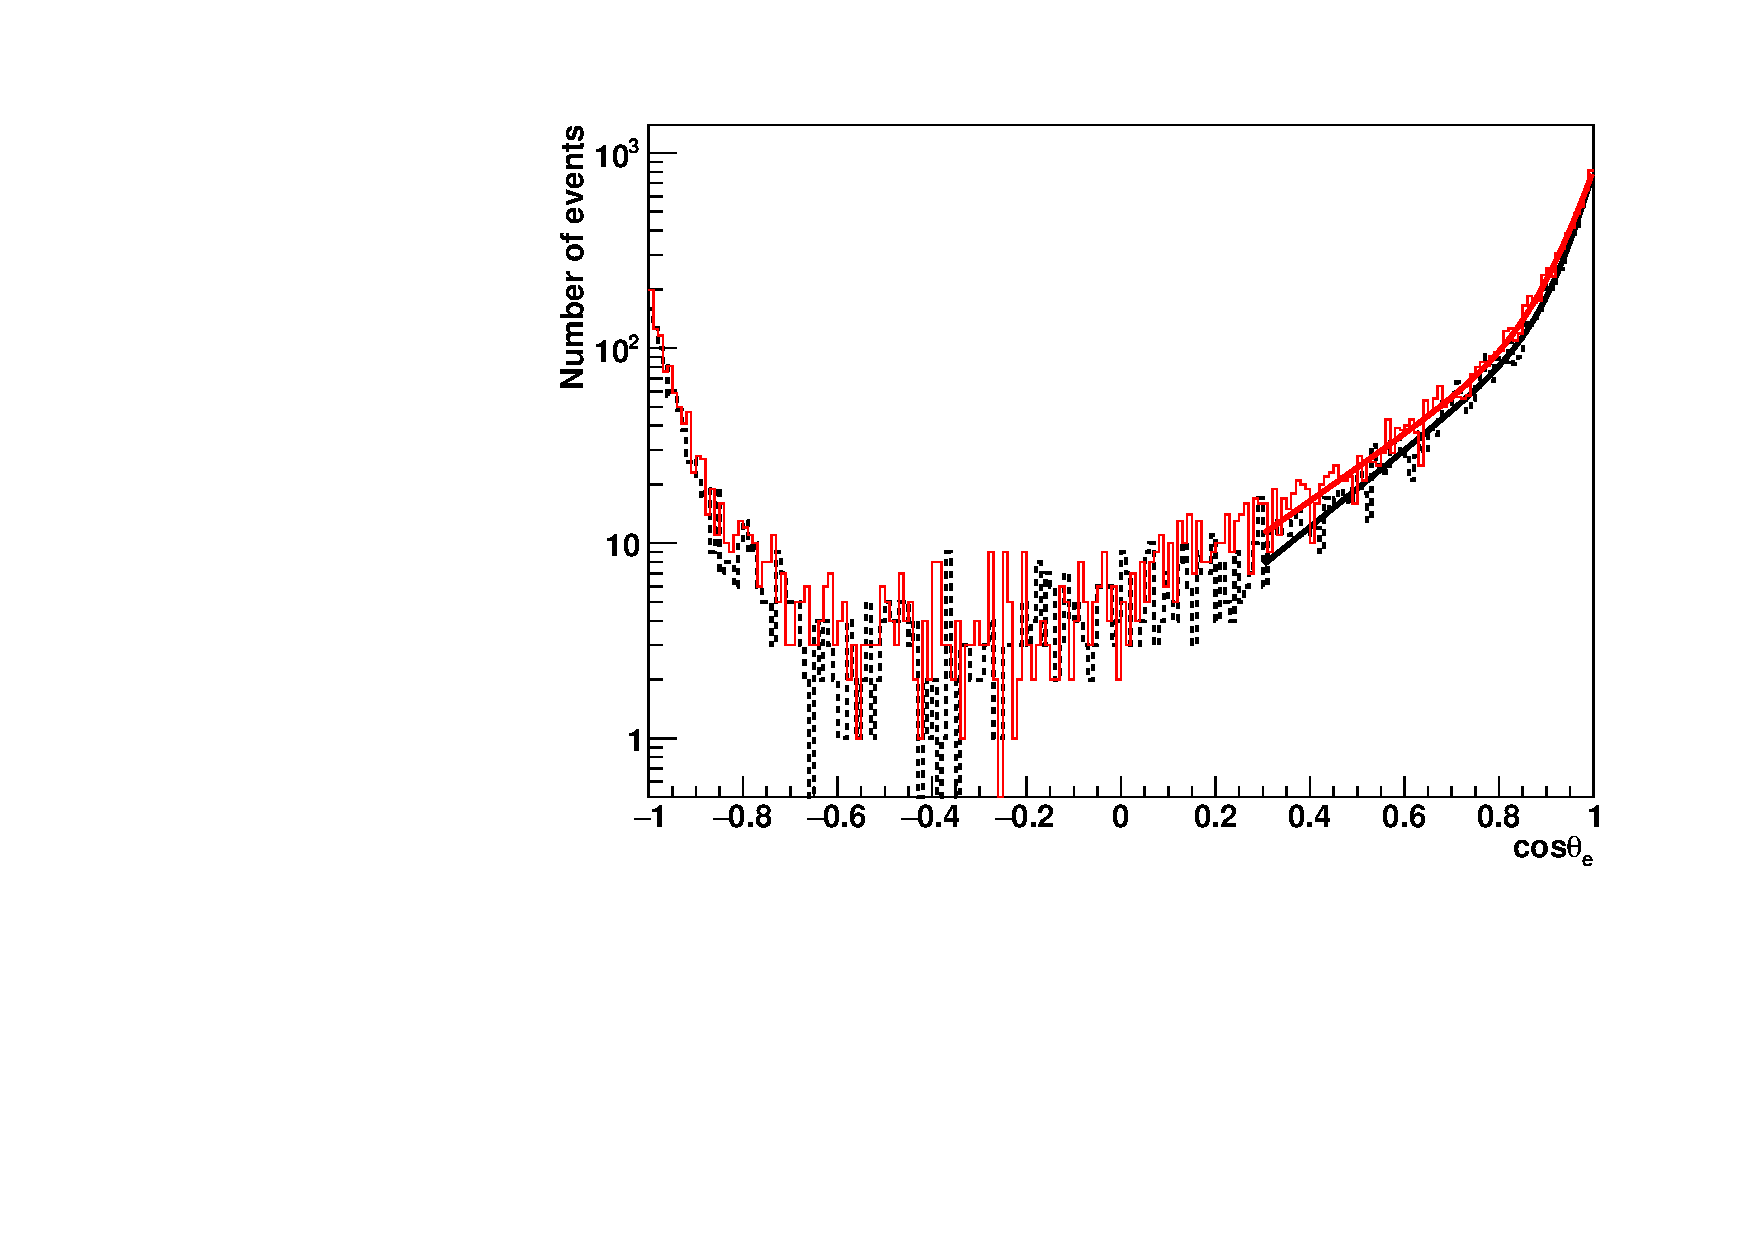
\includegraphics[width=10cm]{16NangularResol.pdf}
	\caption{Angular distributions extracted from the data (red solid line) and the MC (black dashed line); both are reconstructed by the MPW fitter. These distributions are fitted with the angular resolution functions ranging from 0.3 to 1.}
	\label{angularResolMPW}
\end{figure}

\begin{table}[ht]
	\begin{tabular}{cccccccc}%{|p{2.2cm}|p{1.8cm}|p{2cm}|p{2cm}|p{1.8cm}|p{1.1cm}|p{1.1cm}|p{1.1cm}| }
		\toprule
	107055& $\beta_M$ &  $\beta_S$ & $\alpha_M$ & $\chi^2$/ndf & $\cos\theta_{0.5}$ & $\cos\theta_{0.8}$& $\cos\theta_{0.9}$\\
	\hline
	MPW data & 4.15$\pm$0.18 & 19.08$\pm$0.94 & 0.58$\pm$0.02 & 77.1/66 & 0.964 & 0.744 & 0.410 \\
	MPW MC & 4.42$\pm$0.19 & 20.41$\pm$1.01 & 0.56$\pm$0.02 & 83.8/66 & 0.974 & 0.768 & 0.454	 \\	
\hline
	Rat data & 3.76$\pm$0.18 & 17.90$\pm$0.82 & 0.55$\pm$0.02 & 70.5/66 & 0.974 & 0.731 & 0.364 \\
	Rat MC & 4.02$\pm$0.18 & 20.89$\pm$0.92 & 0.54$\pm$0.03 & 94.9/66 & 0.979 & 0.753 & 0.409	\\
		\bottomrule
	\end{tabular}
	\label{angularResolValuesUpdated}
\end{table}

To describe the $\cos\theta_e$ distribution, the angles that contain 50\%, 80\%
and 90\% of the reconstructed events, the $\cos\theta_{0.5}$, $\cos\theta_{0.8}$ and $\cos\theta_{0.9}$ can also be used. Their values are solved numerically by the equation \ref{eq:cosTheta_e} below (take $\cos\theta_{0.5}$ as an example):

\begin{equation}\label{eq:cosTheta_e}
\frac{\int_{\cos\theta_{0.5}}^1 P(\cos\theta_e) d\cos\theta_e}{\int_{-1}^1 P(\cos\theta_e) d\cos\theta_e} = 50\%,
\end{equation}

where $P(\cos\theta_e)$ is the direction resolution function with the best fitted parameters. If these values are large, the $\cos\theta_e$ distribution is sharper and more peaked around +1.

From the results above, the direction resolutions of the MC are always better than the data, due to the ideal situations in the simulations. The MPW and the RAT reconstructions are similar, while the $\beta_M$ values of the MPW are about 10\% higher than the RAT in both of the data and the MC. This indicates the direction resolution of the MPW is slightly better than the RAT.

\subsubsection{Direction Systematics}
For all the internal $^{16}$N scans, the cuts mentioned in the last section were applied on both the data and simulations. Similar to the evaluation of the position uncertainties, the angular resolution function was first fitted with 3 free parameters: $\alpha_M$, $\beta_S$, $\beta_M$. To simplify the calculation in propagating systematics, an average value of the fitted $\alpha_M$ was calculated from all the internal scans (except the three neck scans), as 0.613 for data and 0.585 for MC. With the fixed values of $\alpha_M$, both the data and the MC were refit with $\beta_S$ and $\beta_M$ only. The default fit range is [0.3,1], while for some scans close to the AV, the events can be few after the cuts. For these situations, in order to ensure more than 5000 events were fitted, the fit range was enlarged by moving a 0.1 step to the left until the left value reaches -0.5: $[0.3-0.1\cdot step,1]$.

Fig.~\ref{angularResolScan} shows the results of the fitted $\beta_M$ and $\beta_S$ values for the internal $^{16}$N x, y and z-axes scans. It shows that for most of the scans, the MC results are better than the data. The three Z scans in the neck have the worst direction resolutions due to the asymmetry of the detector geometry. 

\begin{figure}
	\centering
	\subfigure[$^{16}$N x-scan runs.]{\label{angular:xscan}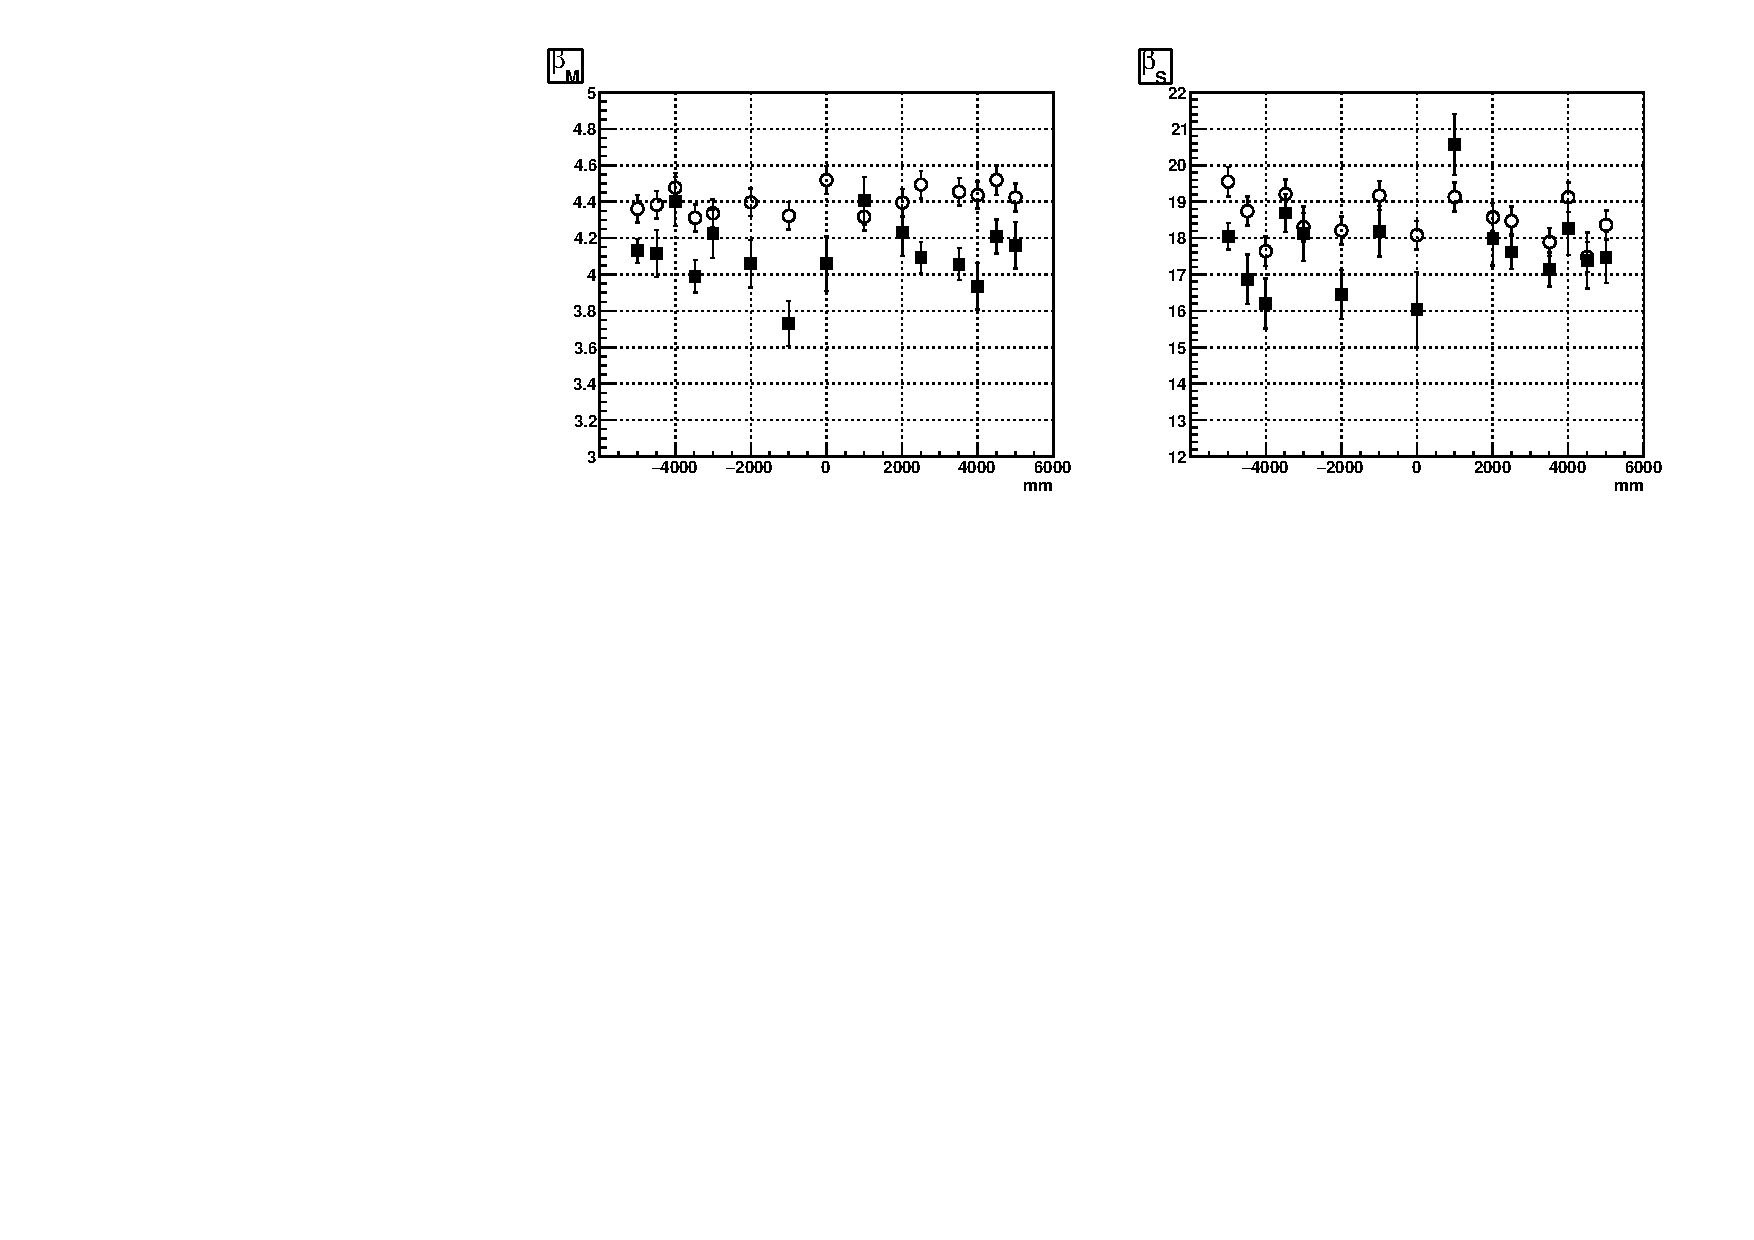
\includegraphics[width=12cm]{16NangularScan_x.pdf}}
	\subfigure[$^{16}$N y-scan runs.]{\label{angular:yscan}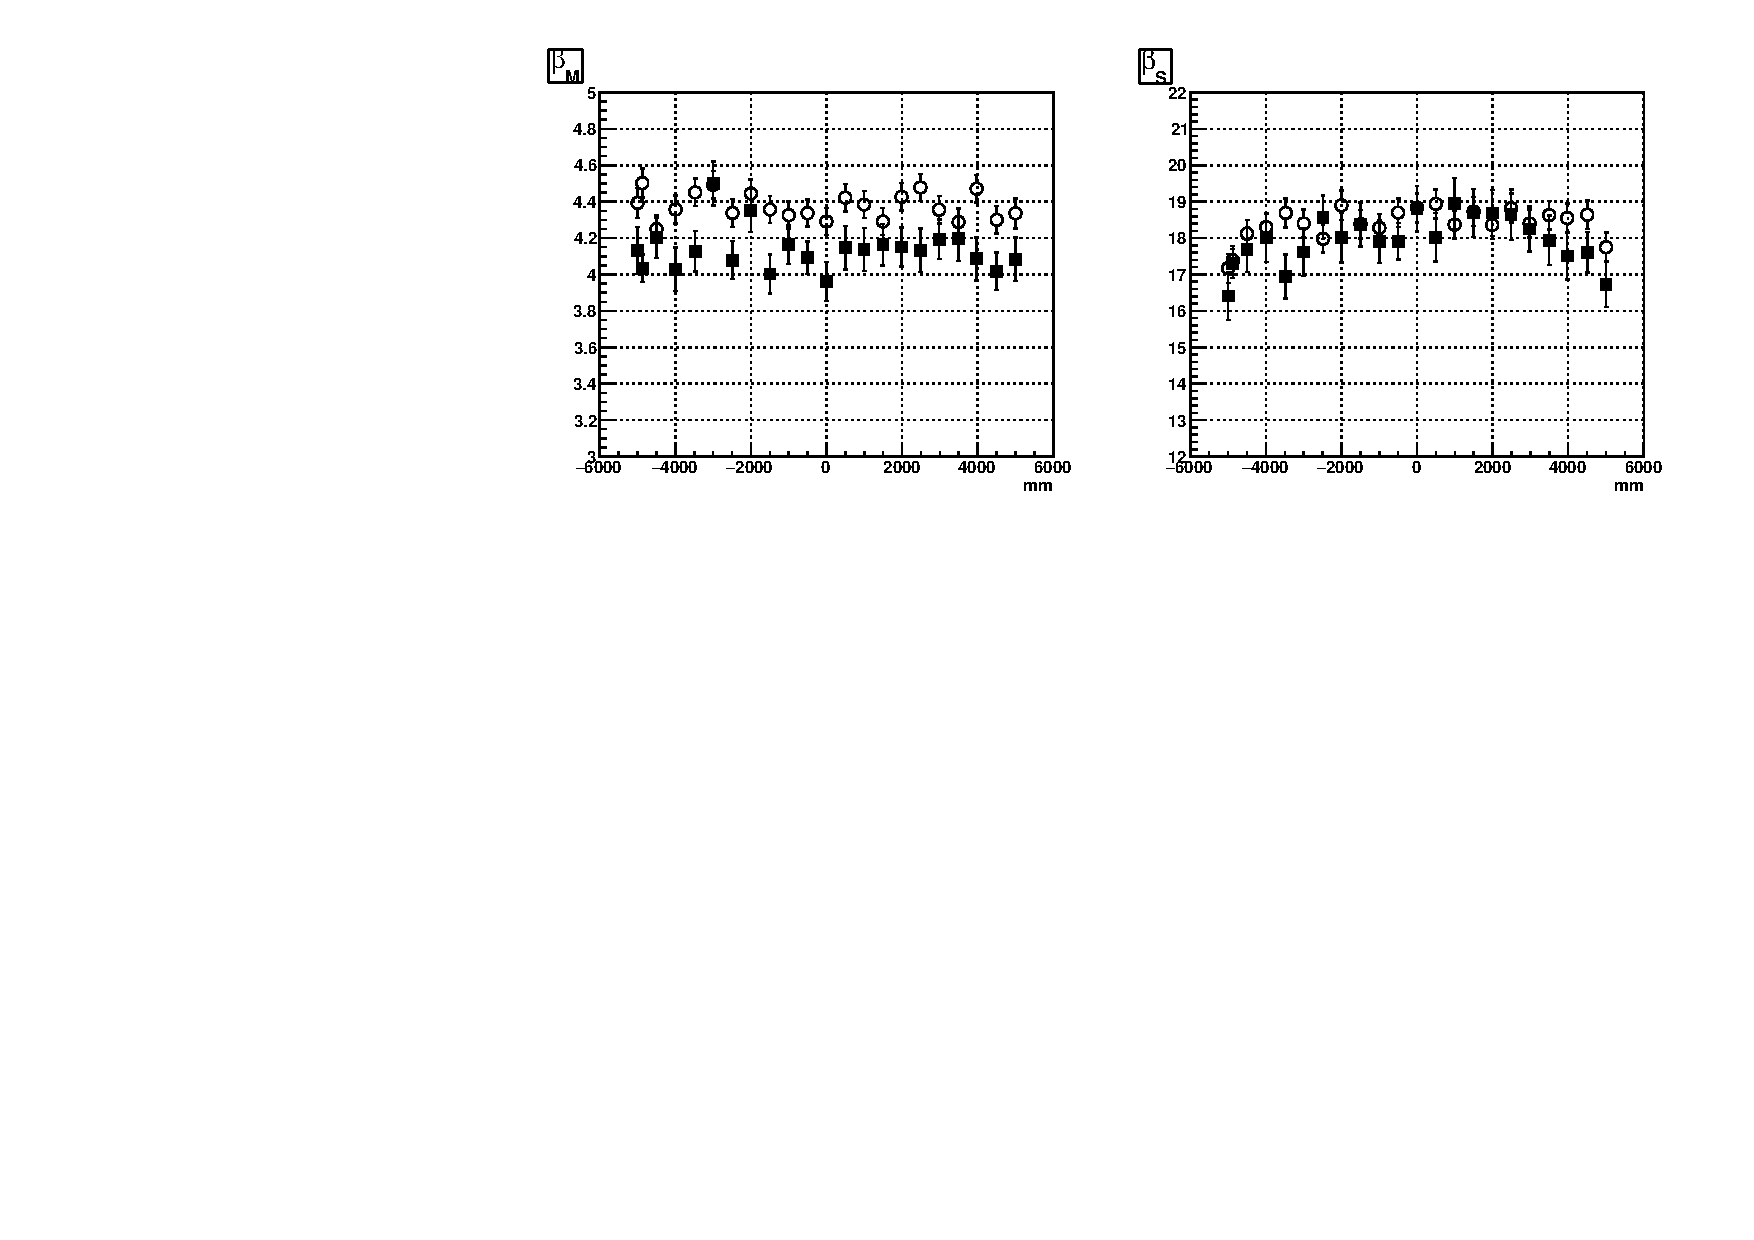
\includegraphics[width=12cm]{16NangularScan_y.pdf}}
	\subfigure[$^{16}$N z-scan runs.]{\label{angular:zscan}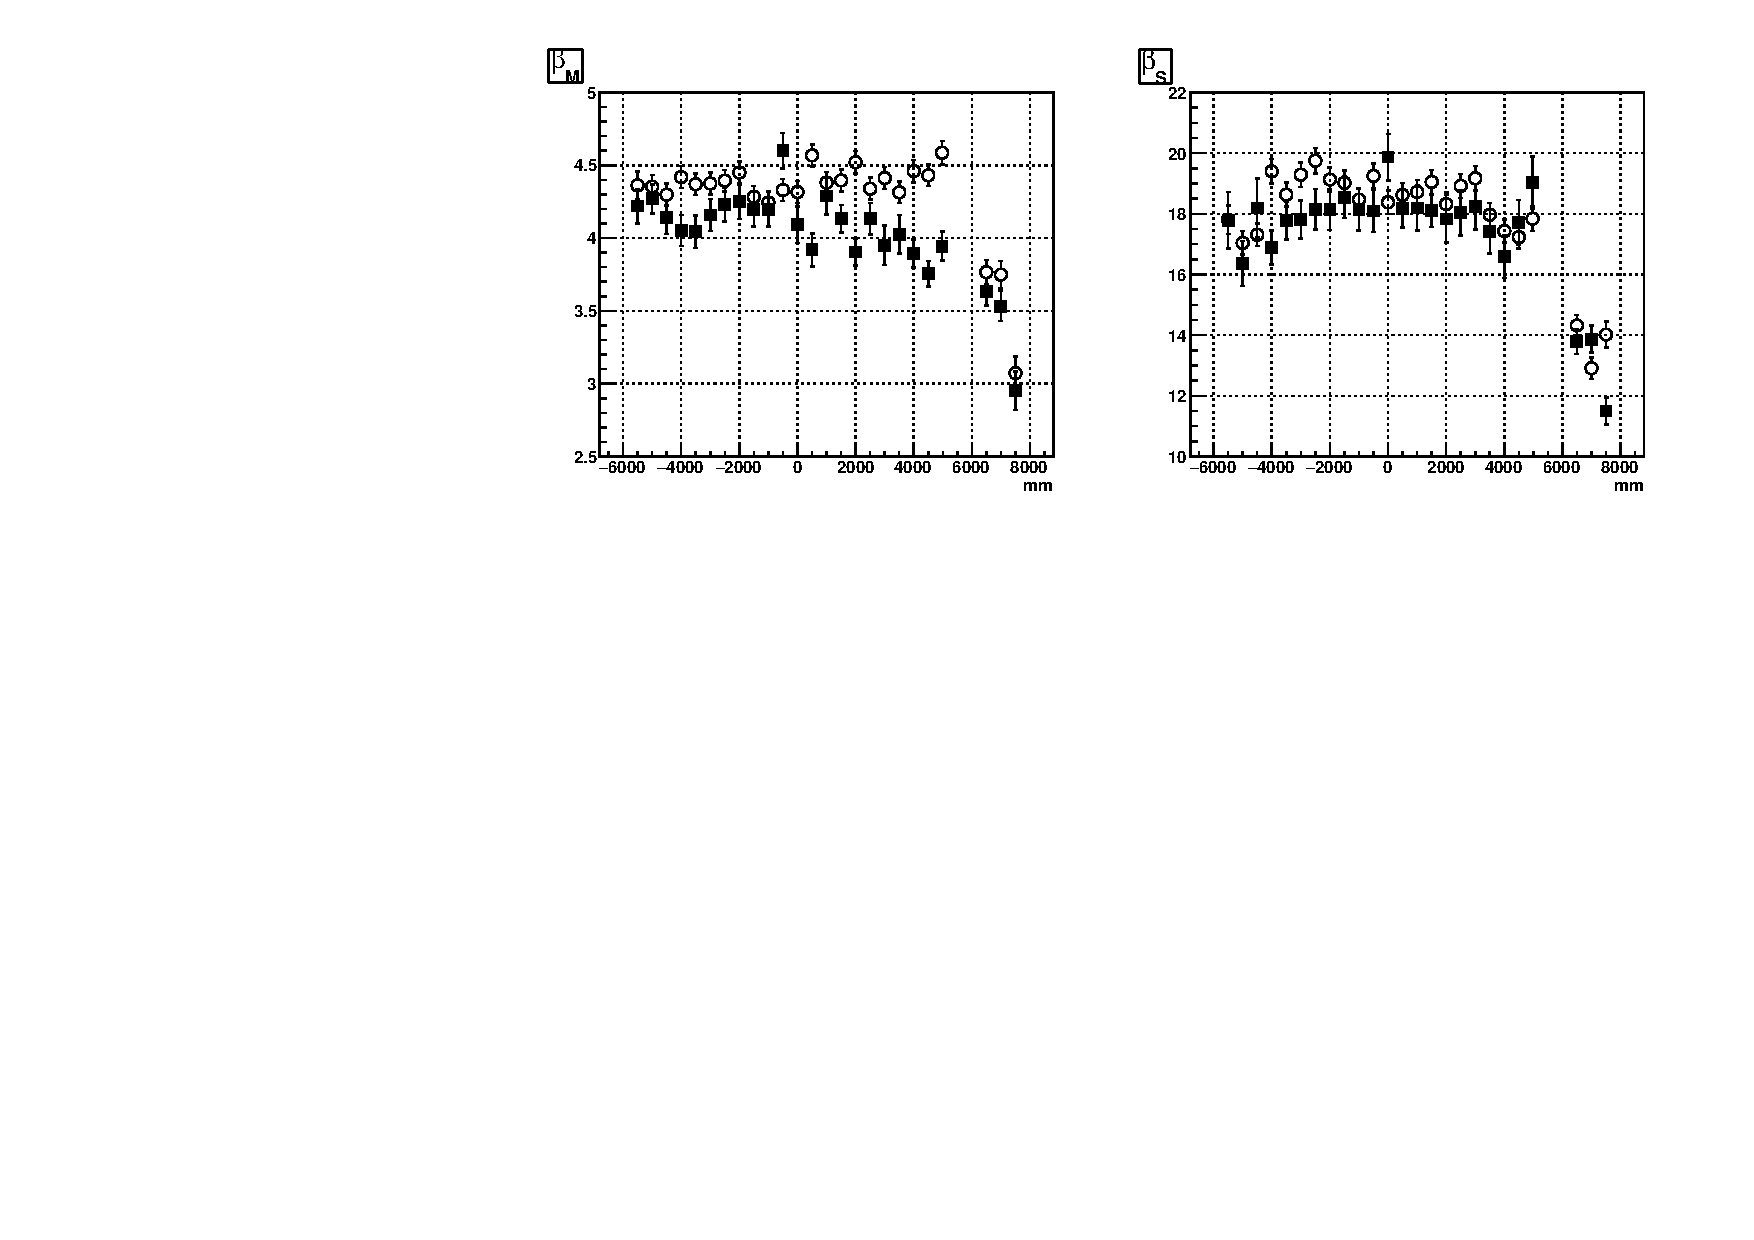
\includegraphics[width=12cm]{16NangularScan_z.pdf}}
	\caption{Fitted direction resolution parameters $\beta_M$, $\beta_S$ for x, y, z-axes scans.}
	\label{angularResolScan}
\end{figure}

The relative difference between data and MC of a fitted resolution quantity $q\pm \delta_q$ is defined as:
\begin{equation}
(\Delta q)_{rel} = \frac{q_{data}-q_{MC}}{q_{MC}}\times 100\%.
\end{equation}

The error of the relative difference is defined as: 
\begin{equation}
\delta_{(\Delta q)_{rel}} = \sqrt{(\frac{\delta_{q_{data}}}{q_{data}})^2+(\frac{\delta_{q_{MC}}}{q_{MC}})^2}\times 100\%.
\end{equation}\label{eq:erors_relativeBiases}

Fig.~\ref{relative_biasesVsPositions} shows the relative differences for the internal x, y, z scans (not using the neck scans).
\begin{figure}[!htb]
	\centering
	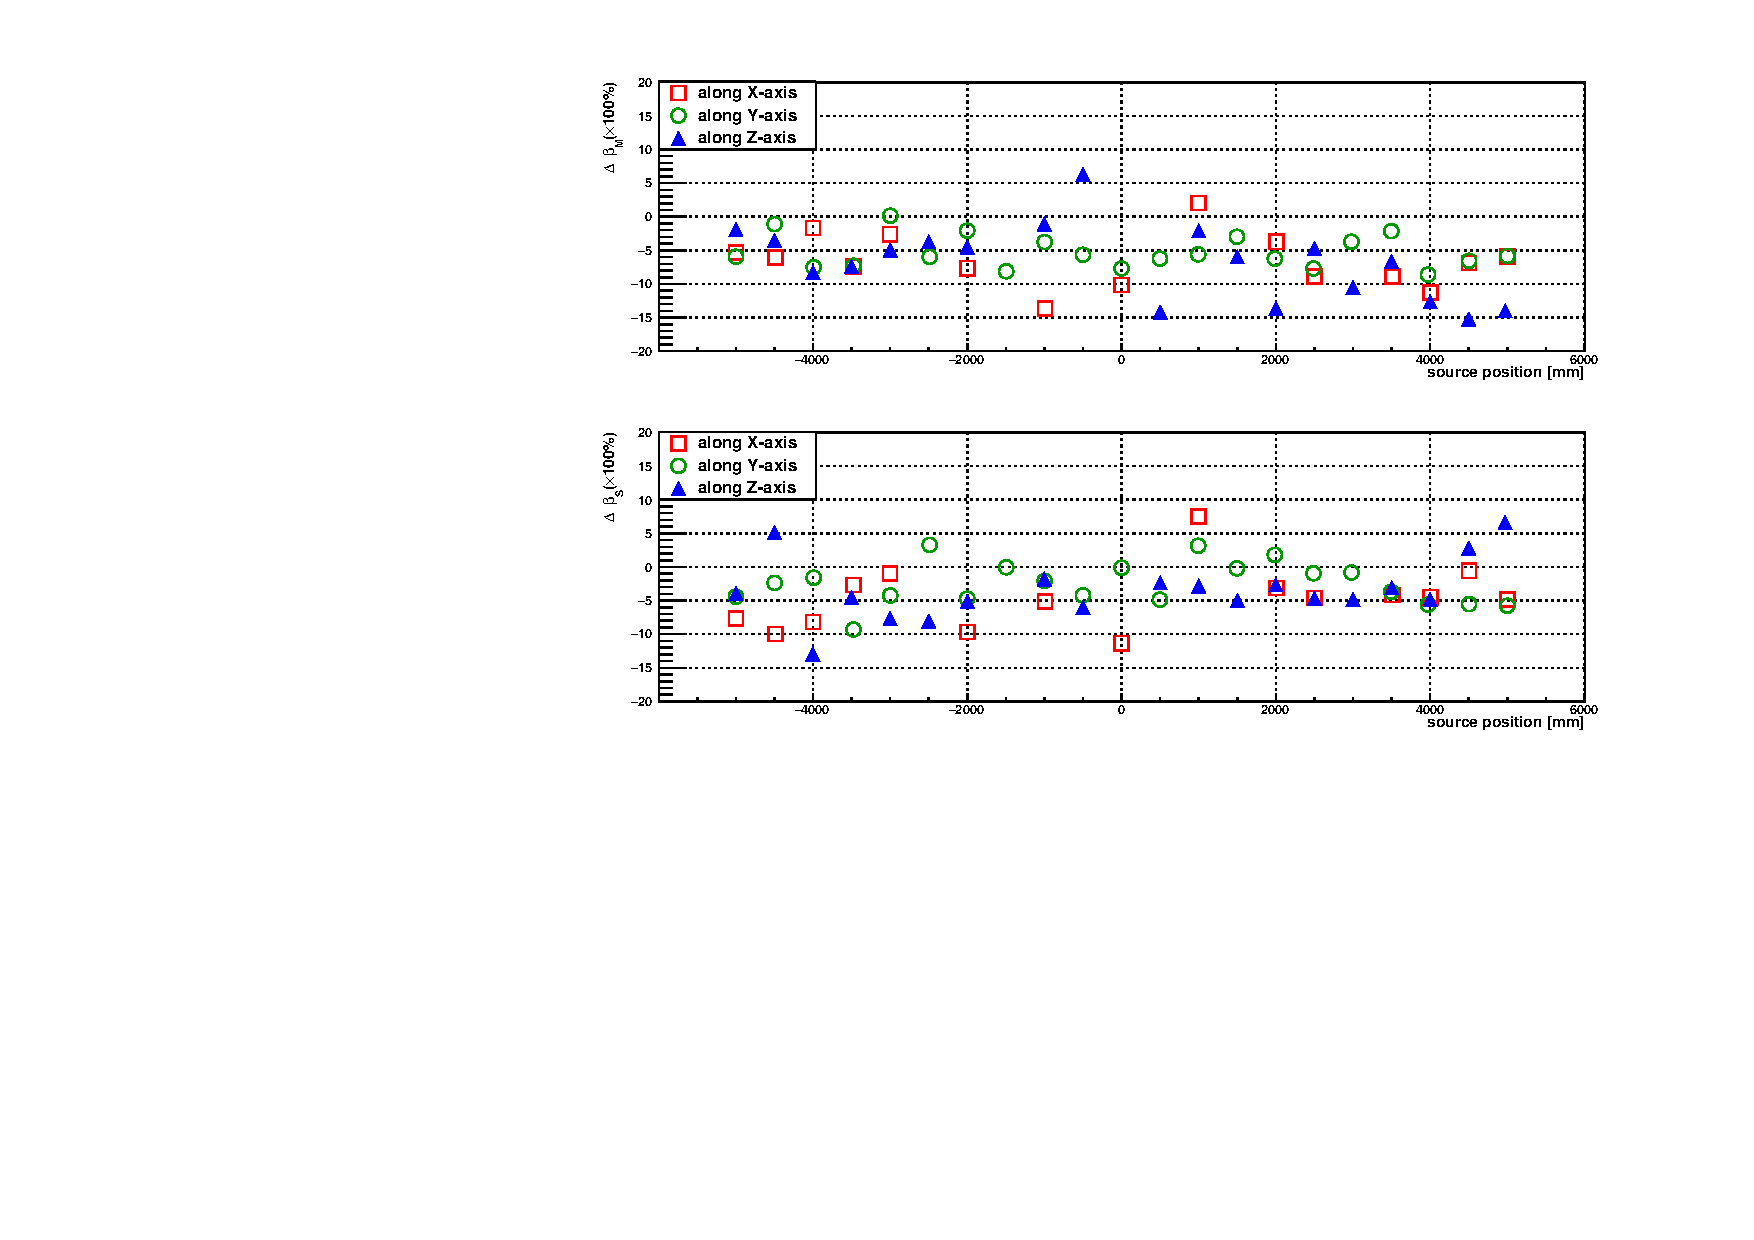
\includegraphics[width=16cm]{angularResol_scanXYZ.pdf}
	\caption{Relative differences of $\beta_M$ and $\beta_S$ as a function of the $^{16}$N source position. For simplicity, the corner scans are not shown in this figure. The red squares represent the results from the x-scan runs; green circles represent the y-scan runs and the blue triangles represent the z-scan runs.}
	\label{relative_biasesVsPositions}
\end{figure}

For the internal x, y, z scans (not using the neck scans) and corner scans (76 runs in total), Fig.~\ref{relative_biases_betaM} and Fig.~\ref{relative_biases_betaS} show the distributions of the $(\Delta \beta_M)_{rel}$ and $(\Delta \beta_S)_{rel}$.
\begin{figure}
	\centering
     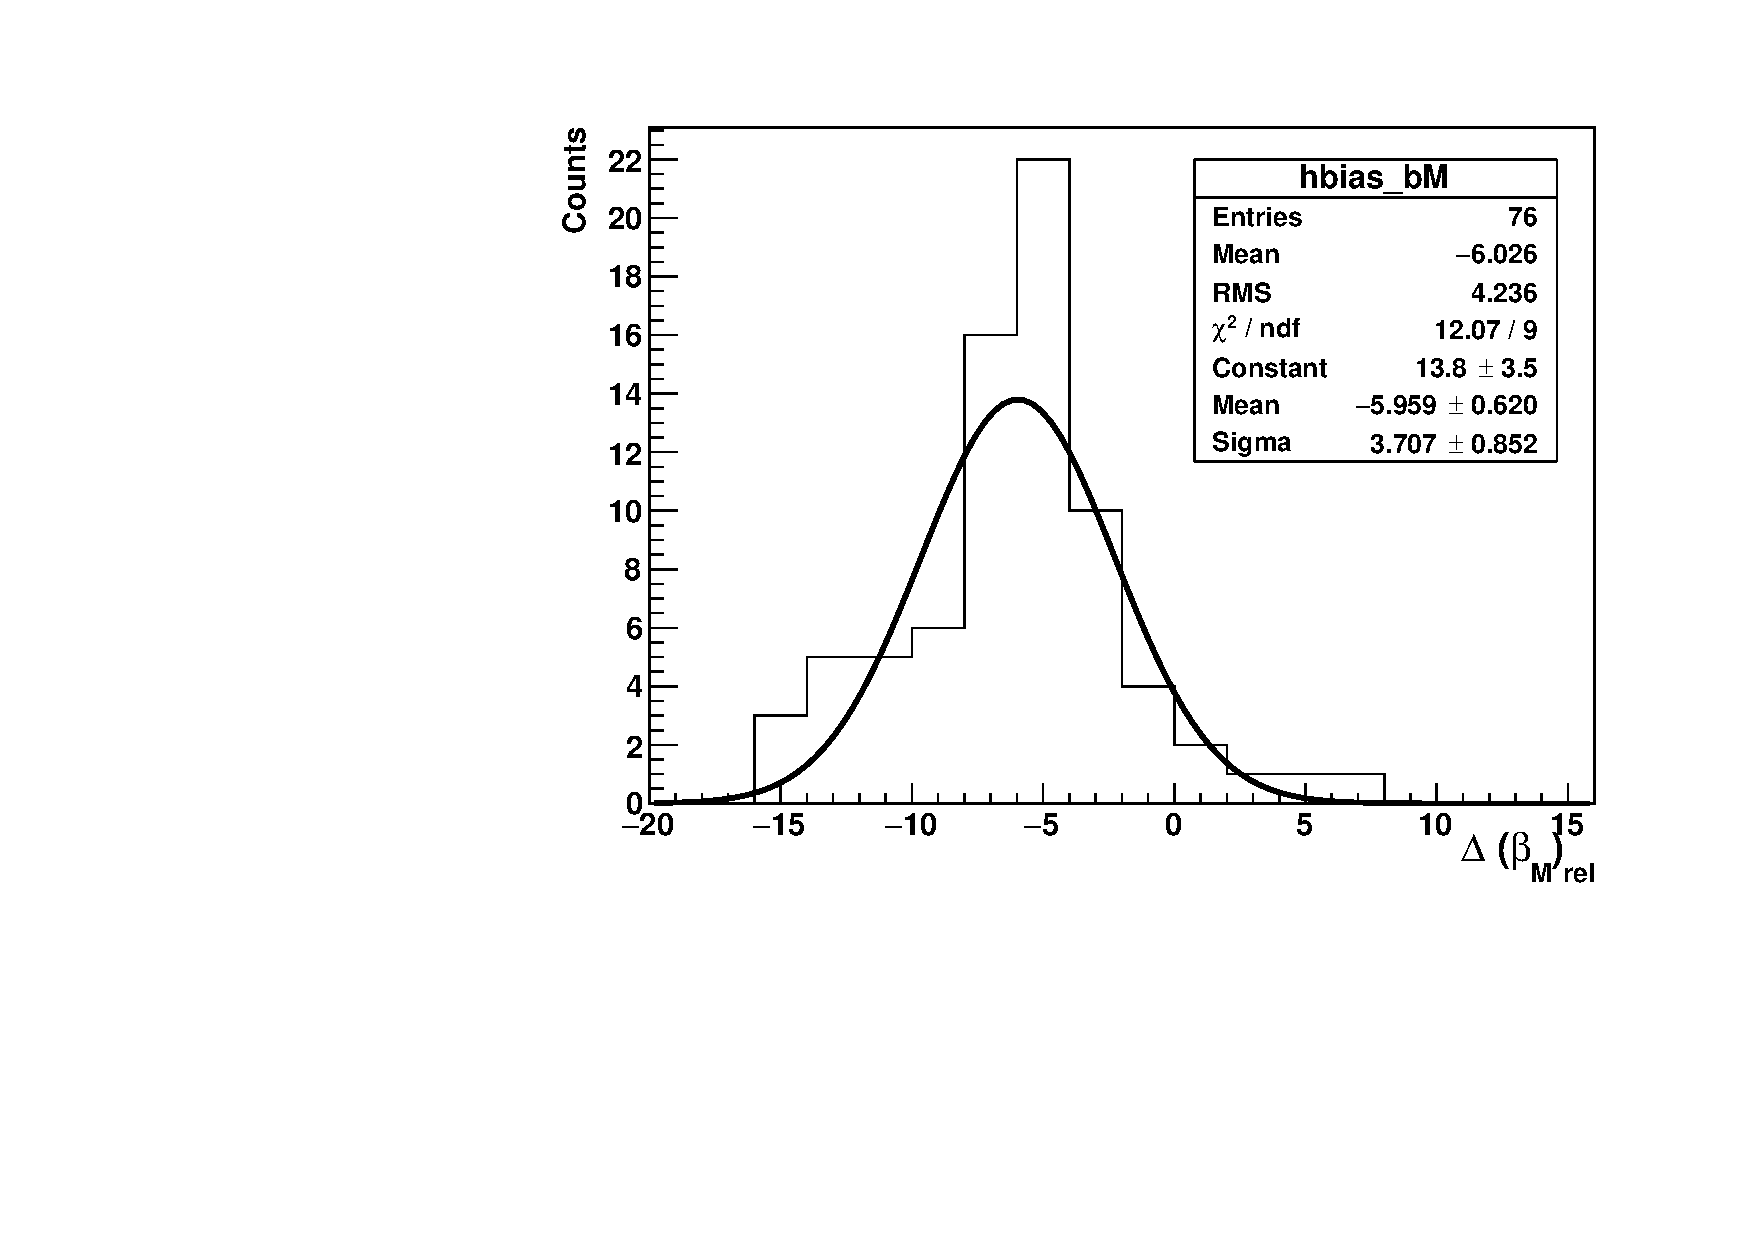
\includegraphics[width=8cm]{relativeBias_betaM.pdf}
	\caption{Relative biases in $\beta_M$ ($\Delta(\beta_M)_{rel}$) for 76 internal scans.}
	\label{relative_biases_betaM}
\end{figure}
\begin{figure}
		\centering
	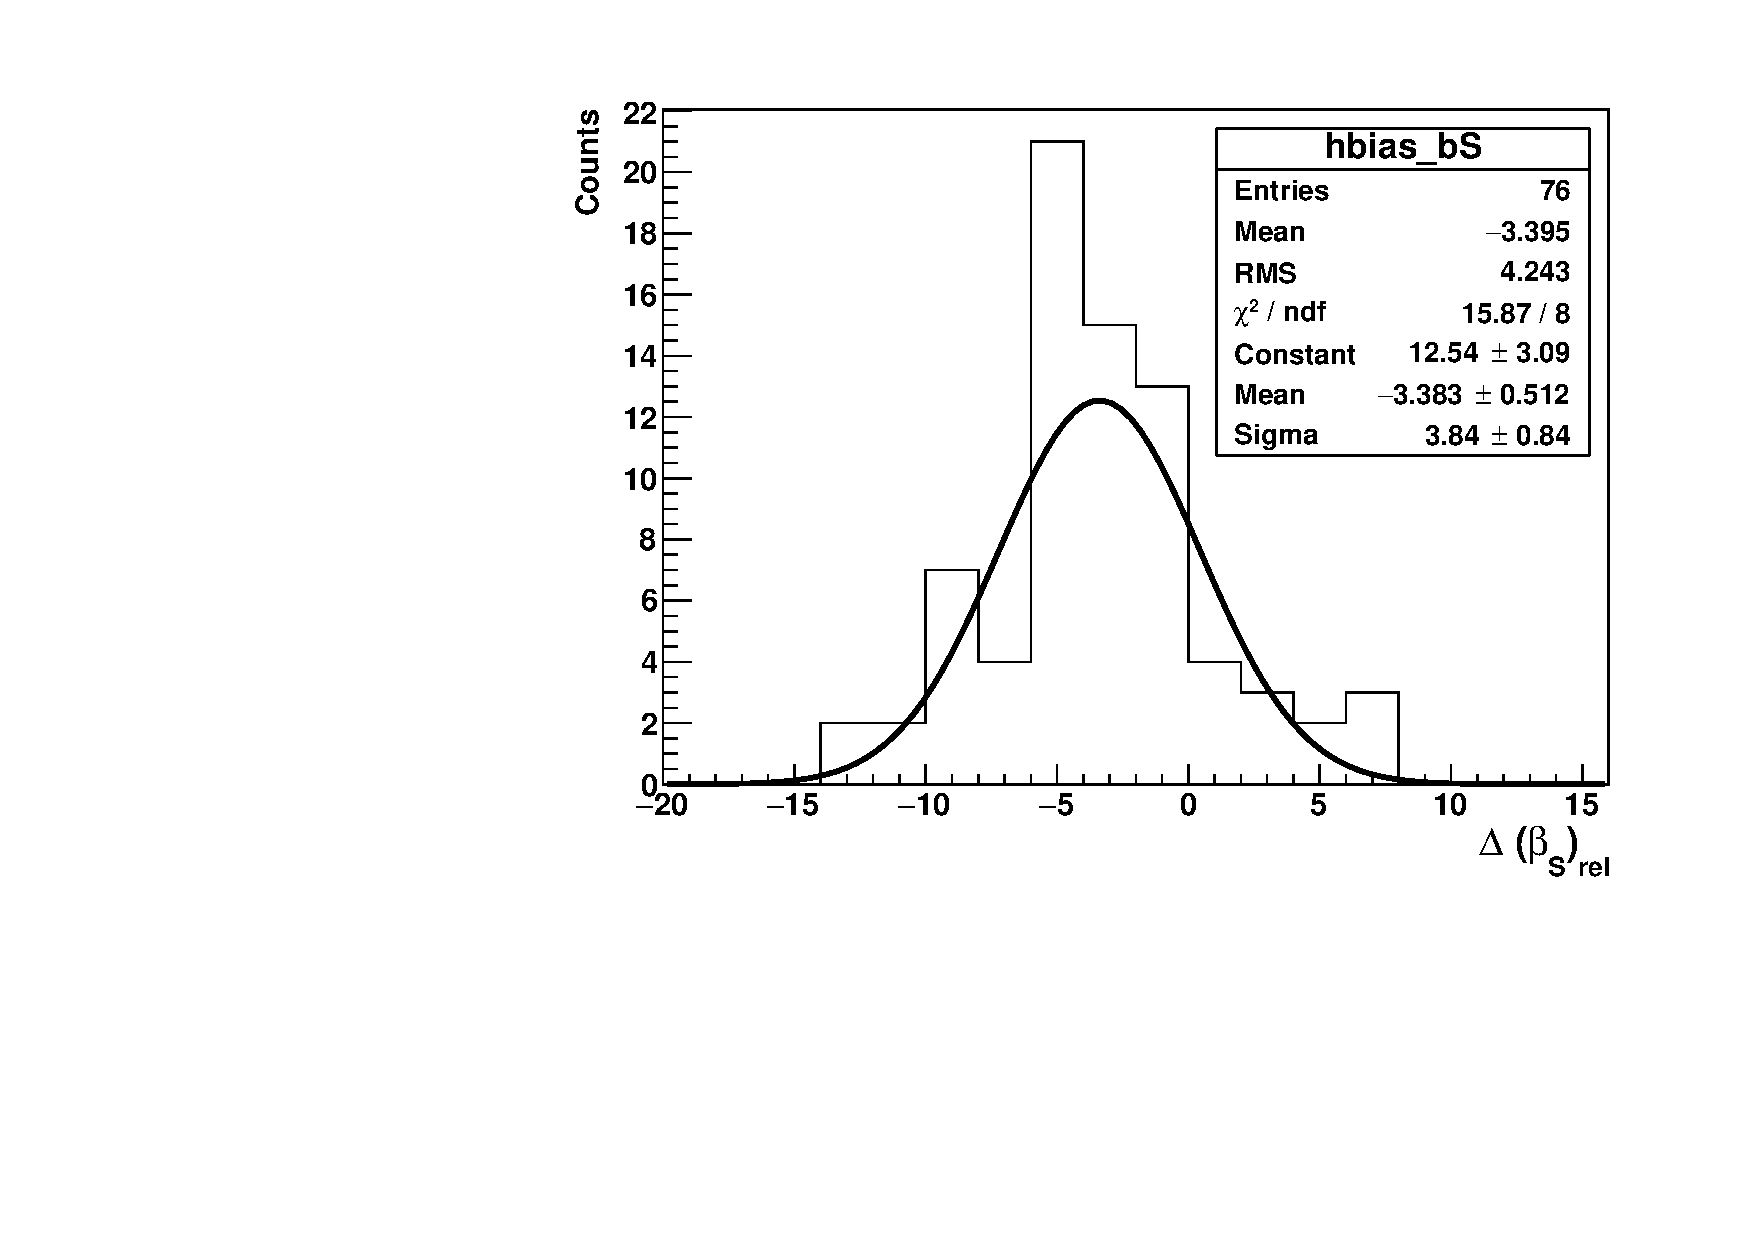
\includegraphics[width=8cm]{relativeBias_betaS.pdf}
\caption{Relative biases in $\beta_S$ ($\Delta(\beta_S)_{rel}$) for 76 internal scans.}
\label{relative_biases_betaS}
\end{figure}
	
Therefore, taking the Gaussian means and resolutions, $\Delta(\beta_M)_{rel}=-5.959\pm 3.707\%$ and $\Delta(\beta_S)_{rel}=-3.383\pm 3.840\%$. To be conservative, taking the largest and smallest values among $\Delta(\beta_M)_{rel}$ and $\Delta(\beta_S)_{rel}$, the negative and positive values of the direction systematic ($\delta_\theta$) are obtained as $\delta_\theta=-0.097/0.005$.

To propagate the uncertainties of $\beta$ to the direction resolution, a first-order approximation function was derived by the SNO collaboration\cite{drouin2012three}:
\begin{equation}\label{remapTheta}
\cos\theta'=1+(\cos\theta_{sun}-1)(1+\delta_{\theta}).
\end{equation} 

This angular remapping function is used to smear the angular distributions for systematic studies. In the next chapter, it will be applied on the angular distribution of solar neutrino data. 

\subsection{$\beta_{14}$ and Its Systematic}

Fig.~\ref{N16beta14} shows the $\beta_{14}$ distributions for the central run-107055 data and MC, reconstructed by the MPW fitter and the official RAT fitter. The $\beta_{14}$ is calculated based on the reconstructed position, time and direction of an event while the $\beta_{14}$ distributions from the MPW and the RAT fitter results are consistent. However, both of the two fitters show a discrepancy between the data and the MC. This discrepancy can be caused by an inaccurate modeling of the Cherenkov process in the Geant4 simulation\cite{dunmore2004separation,beta14discrepancy}.

\begin{figure}[htbp]
	\centering
	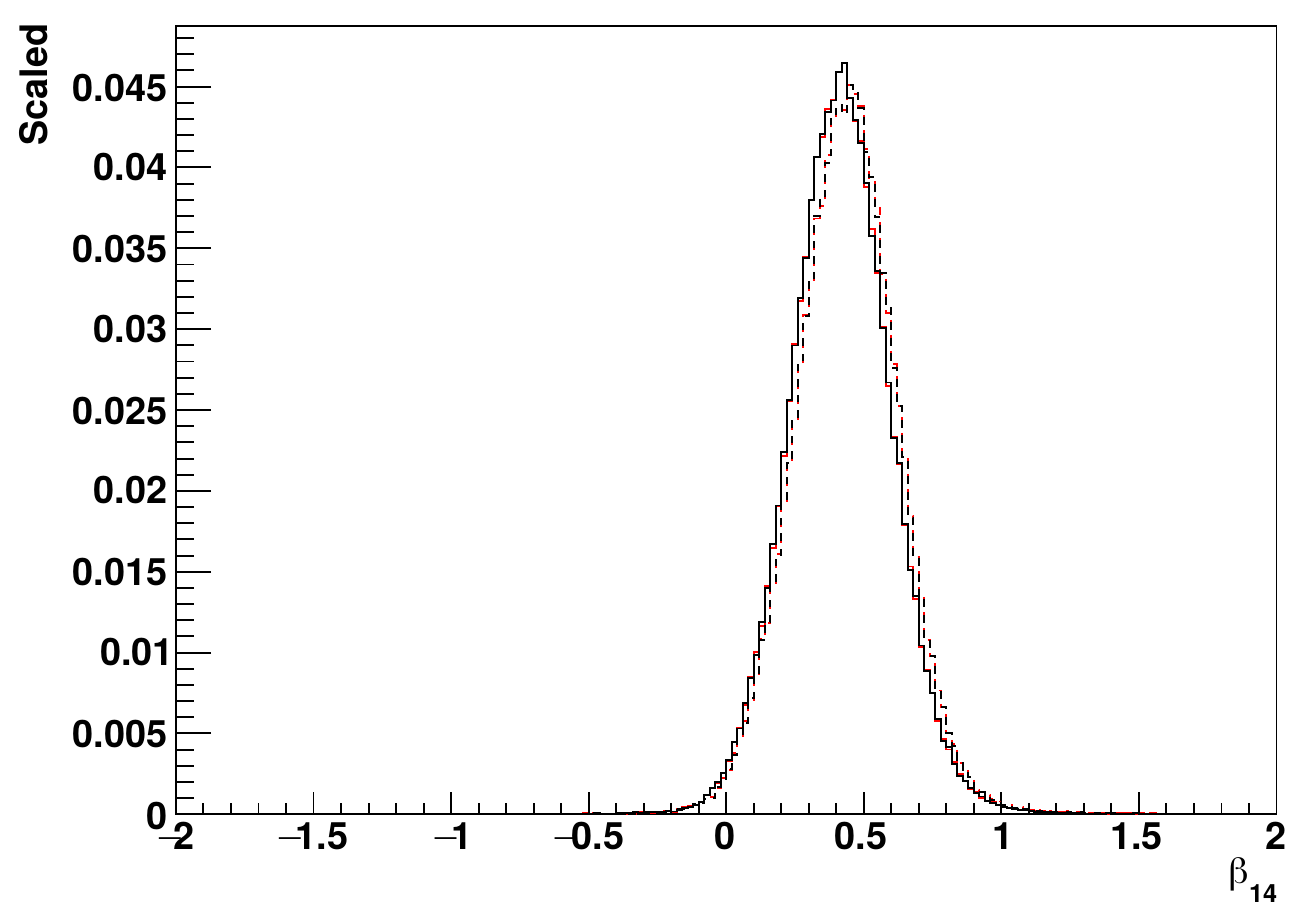
\includegraphics[width=8cm]{N16_beta14_107055.png}
	\caption{Distributions of $\beta_{14}$ for the $^{16}$N central run-107055. Dashed lines for the MC and solid lines for data; red for the MPW fitter processed results and black for the RAT results.}
	\label{N16beta14}
\end{figure}

\begin{figure}[htbp]
	\centering
	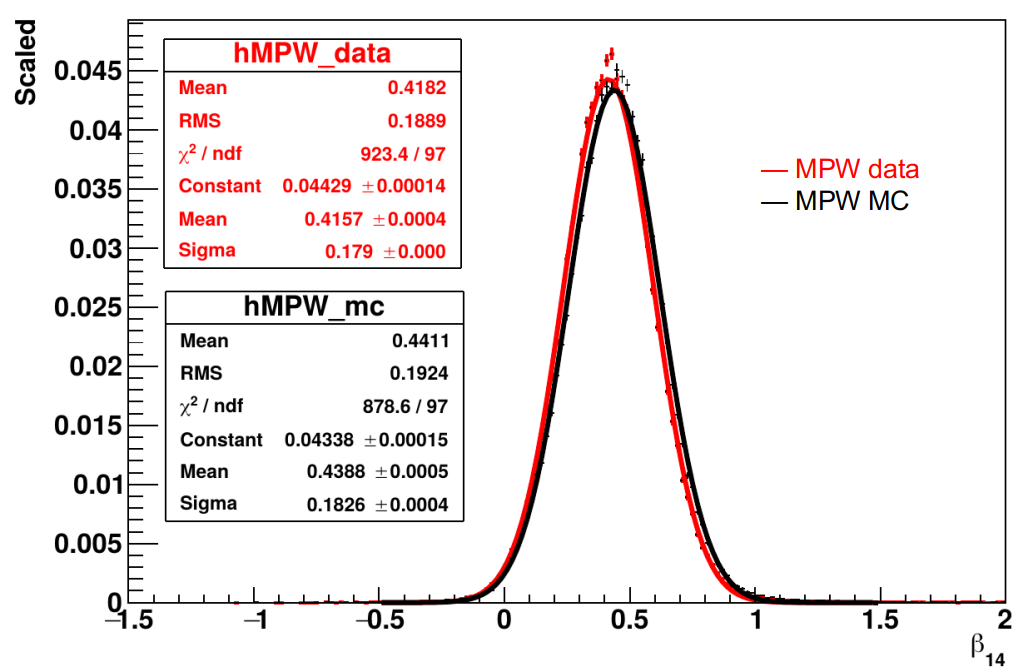
\includegraphics[width=8cm]{N16FitMPW_beta14_107055.png}
	\caption{Comparisons of the $\beta_{14}$ for the data and the MC. Both of the distributions are the MPW processed results and are fitted with Gaussian distributions in a region of $[-0.5,1.5]$. The data shows a smaller mean value (0.4157) than the MC (0.4388).}
	\label{N16beta14MPW}
\end{figure}

\begin{figure}[htbp]
	\centering
	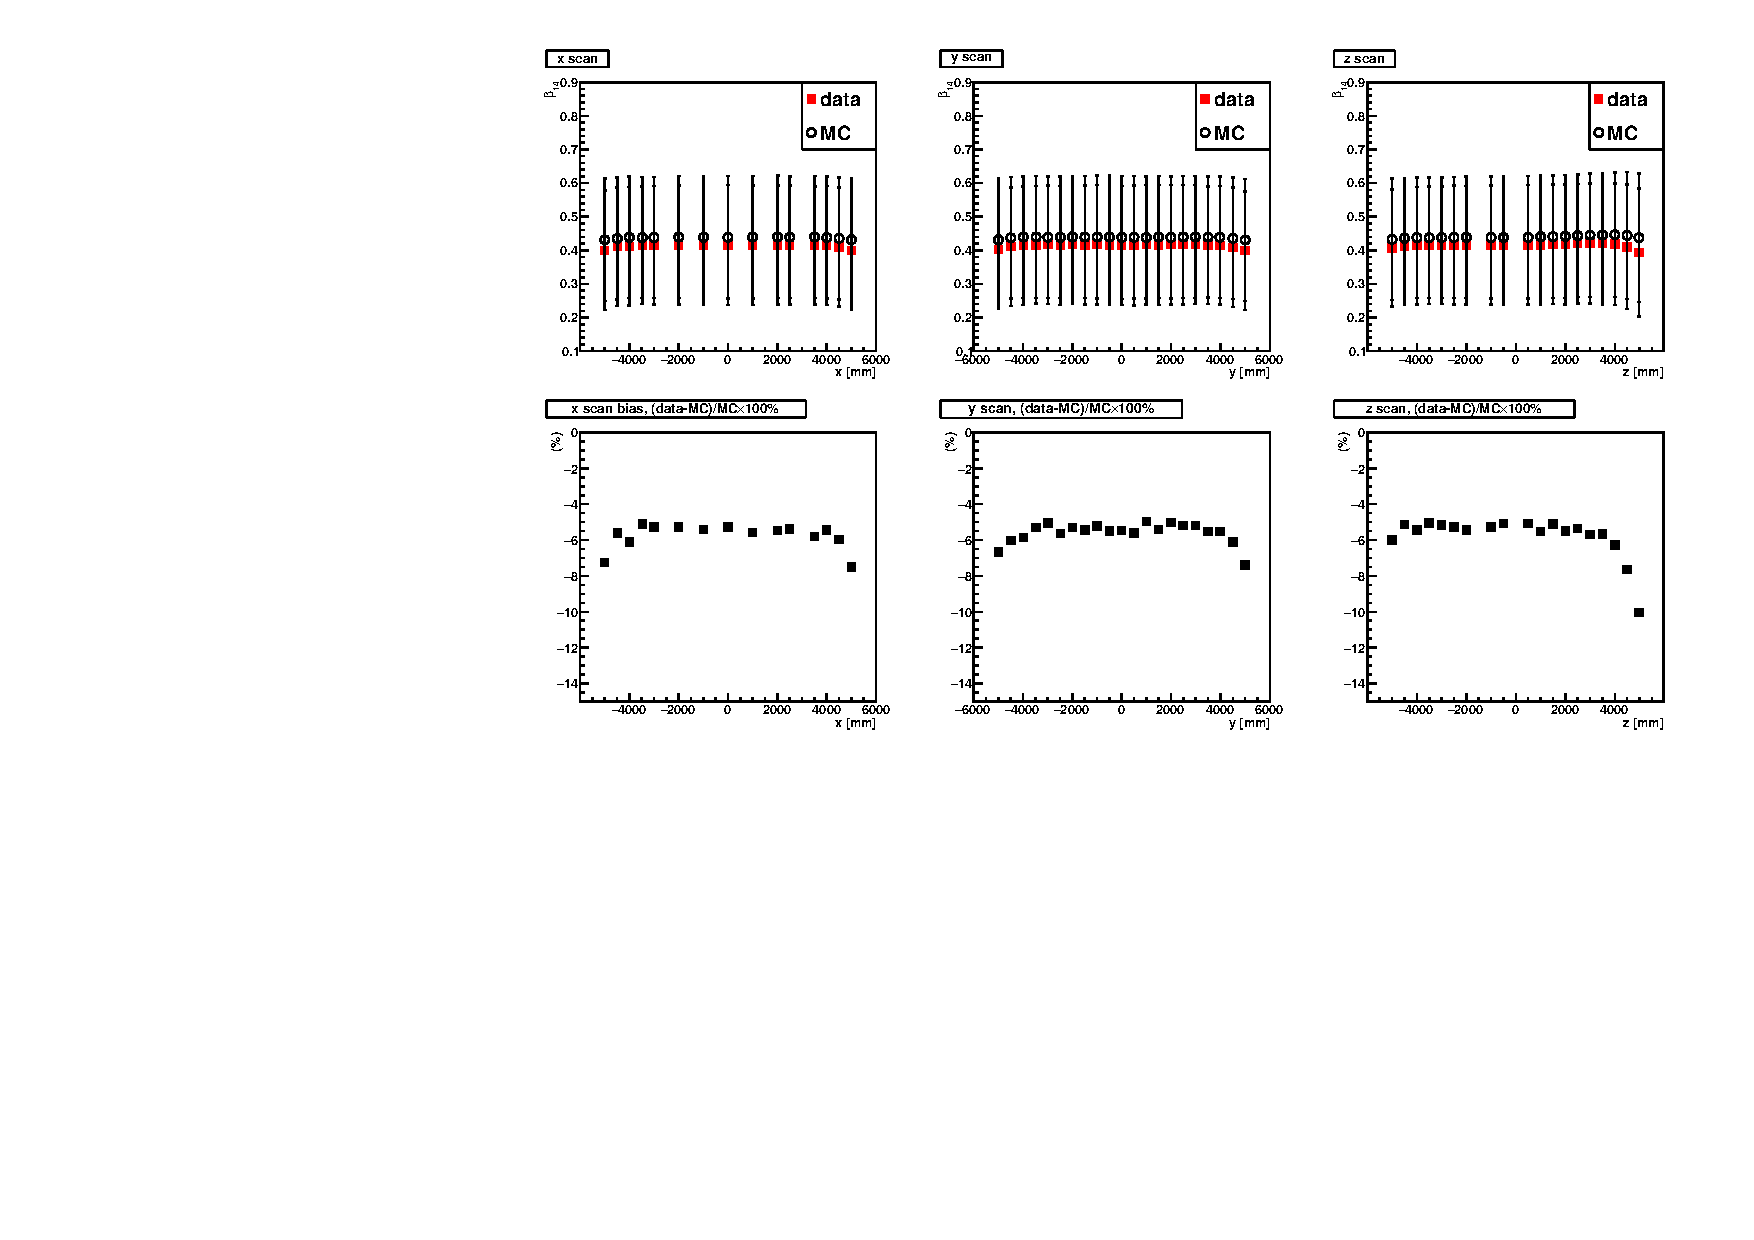
\includegraphics[width=15cm]{beta14_allScans.pdf}
	\caption{$\beta_{14}$ systematic for various $^{16}$N scans.}
	\label{beta14_scans}
\end{figure}

\begin{figure}[htbp]
	\centering
	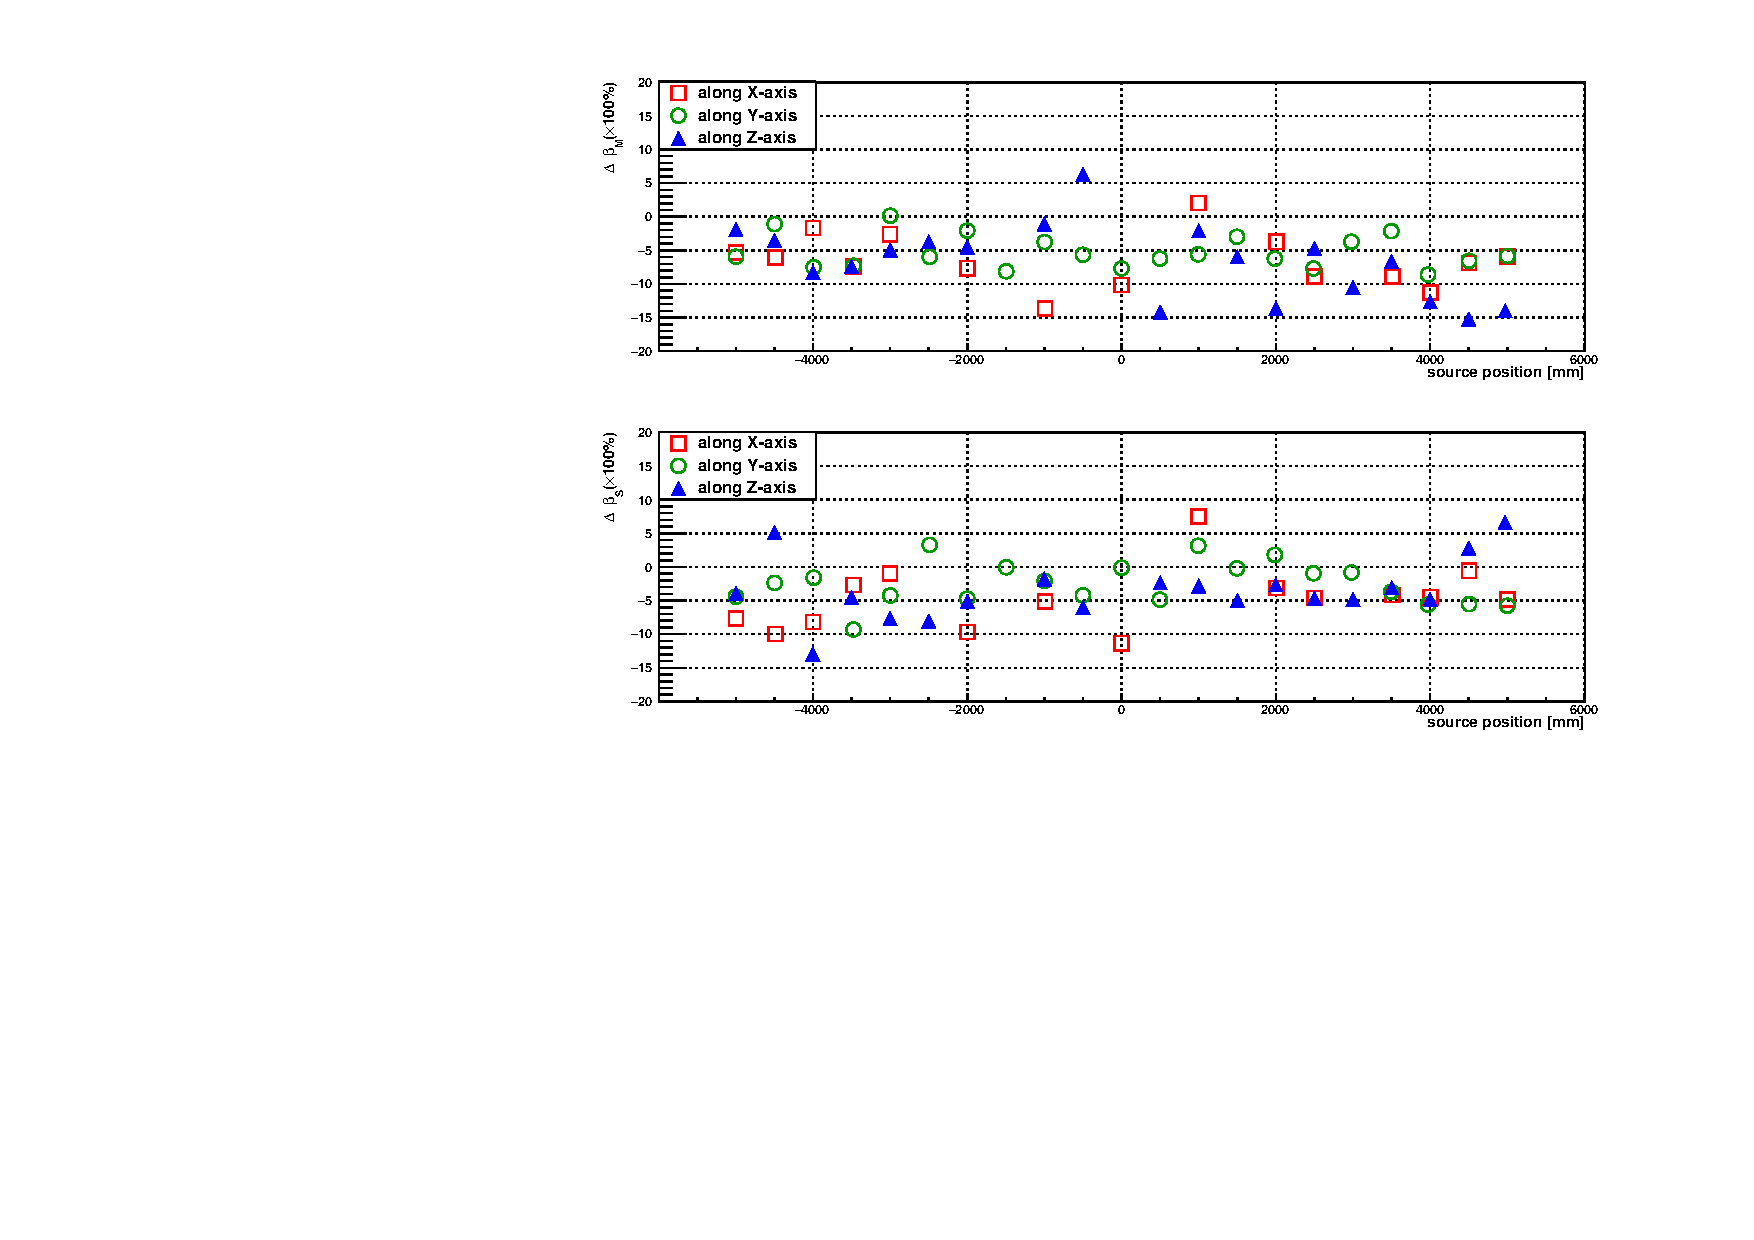
\includegraphics[width=16cm]{angularResol_scanXYZ.pdf}
	\caption{$\Delta\beta_{M}$ (top) and $\Delta\beta_{S}$ (bottom) systematic for various $^{16}$N scans along three axes.}
	\label{xyzScans}
\end{figure}

Discussions for the external scan runs.

For external scans, the radial cuts were not applied. 

%\begin{figure}[!htb]
%	\centering
%	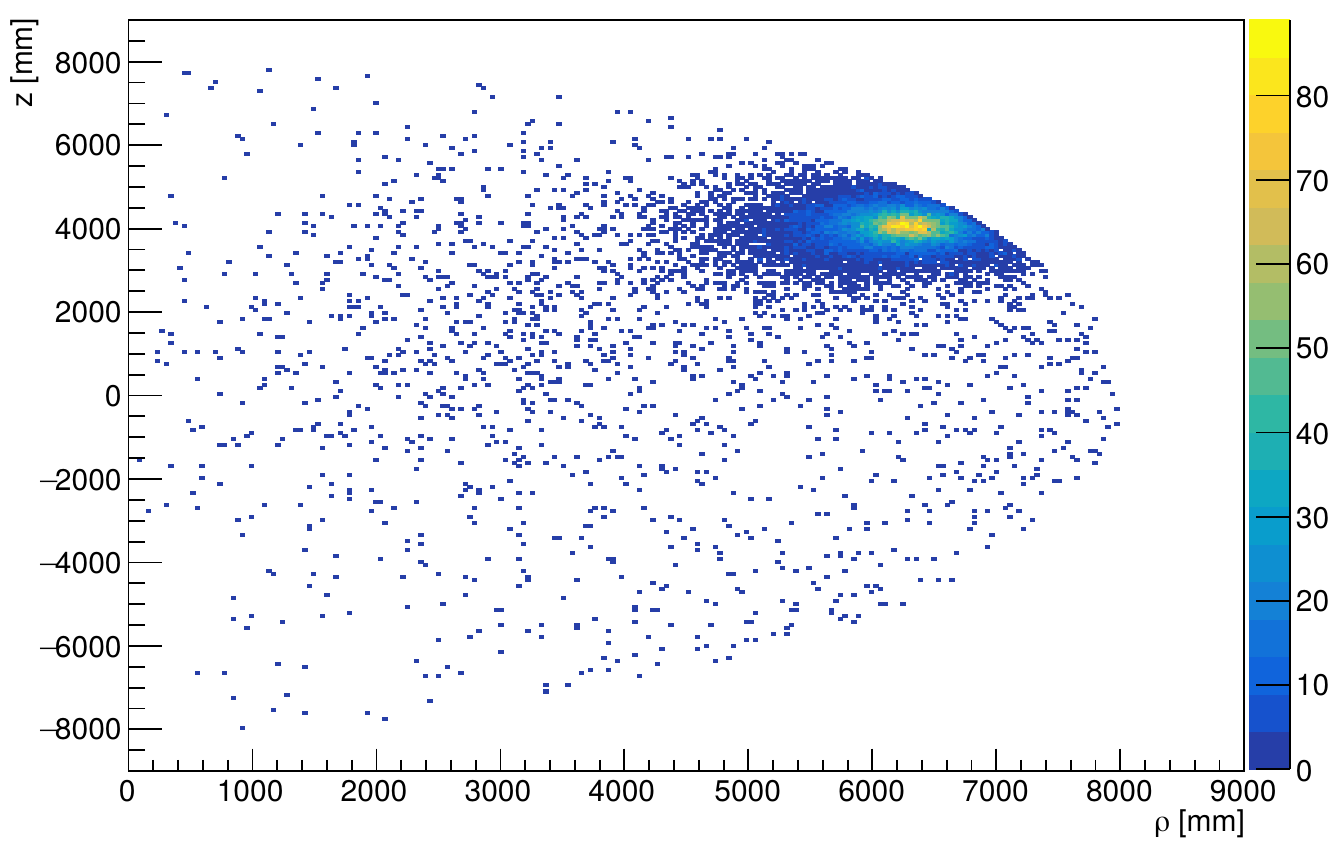
\includegraphics[width=8cm]{N16_external_111230_rhoZ.png}
%	\caption{$^{16}$N external run-111230 with a nominal position at [-5861,-2524,4001] mm; MPW results.}
%	\label{16Nexternal}
%\end{figure}

\subsection{Energy Reconstruction Evaluation}
\subsubsection{Energy Figure of Merits}\label{sect:energy_fomTest}
Three energy FoM quantities: $G_{test}$, $U_{test}$ and $Z_{factor}$ were introduced in \ref{sect:energy_fom}.
Here I used the MC simulations as well as the data of the $^{16}$N central run-107055 to check the effects of the cuts on FOM quantities to reduce the energy biases. The sacrifices of the events were calculated. 

%Then the data of the same run were used to check the ratios of the number of the events which were cut off by the FOM quantities. 

\begin{itemize}
	\item[$\bullet$]$U_{test}$:
	Fig.~\ref{energyFOM_Utest} shows $U_{test}$ vs. energy biases. A cut of $0.61<U_{test}<0.95$ was suggested by the collaboration, to remove the events were mostly caused by the source encapsulation. This cut removes 0.38\% of MC events and 0.34\% of data events.
	\begin{figure}[!htb]
		\centering
		%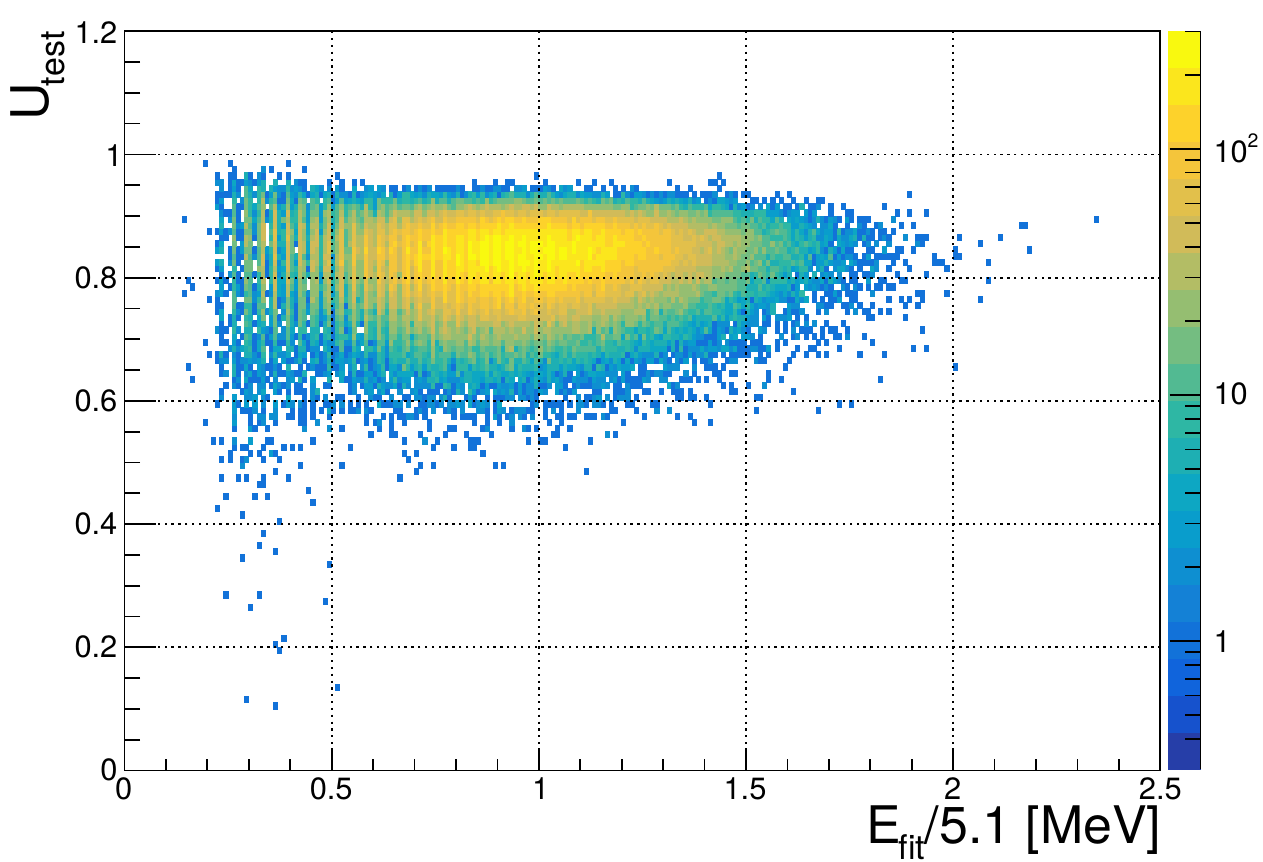
\includegraphics[width=8cm]{Utest_data_N16_107055.png}
		\subfigure[MC]{ 
			\begin{minipage}[t]{0.5\textwidth}
				\centering
				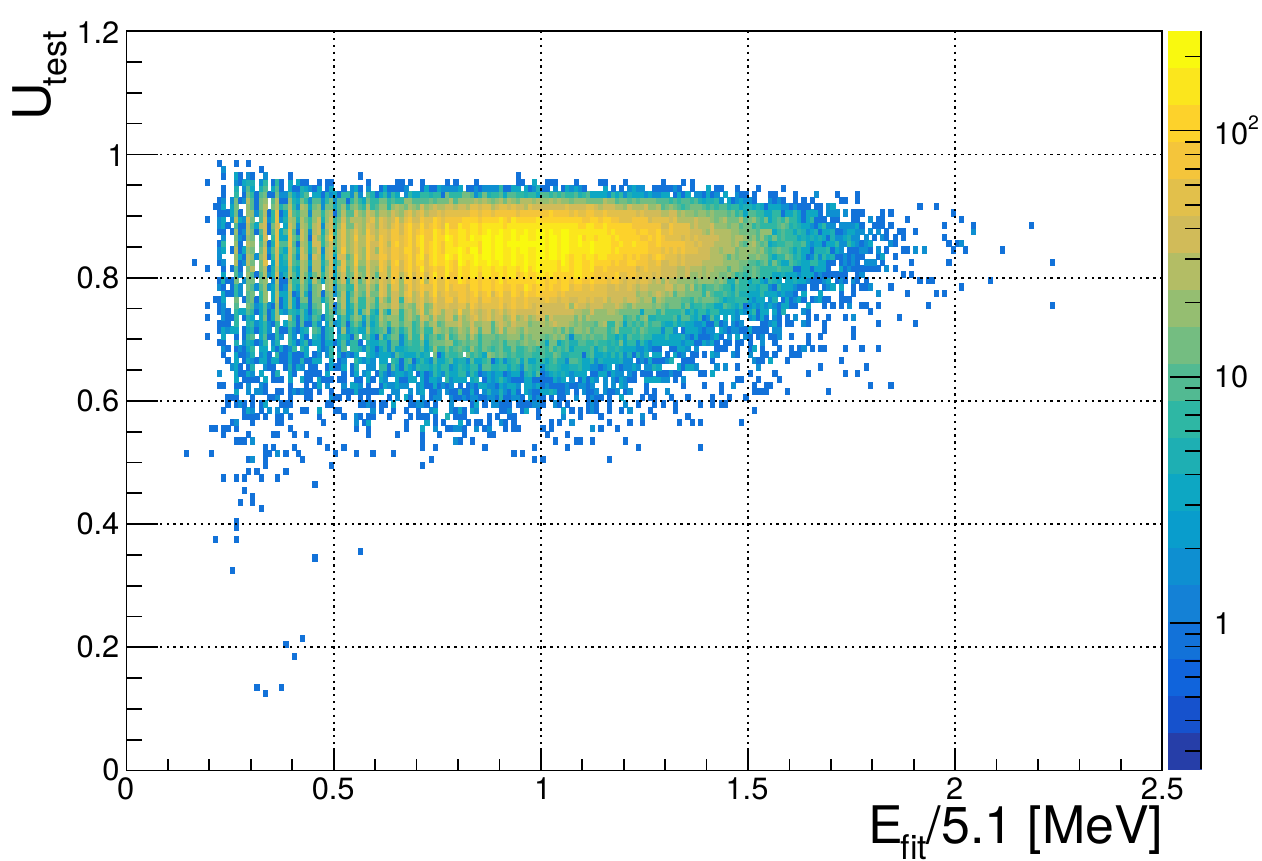
\includegraphics[width=7.5cm]{Utest_MC_N16_107055.png}
			\end{minipage}
		}
		\subfigure[data]{ 
			\begin{minipage}[t]{0.4\textwidth}
				\centering
				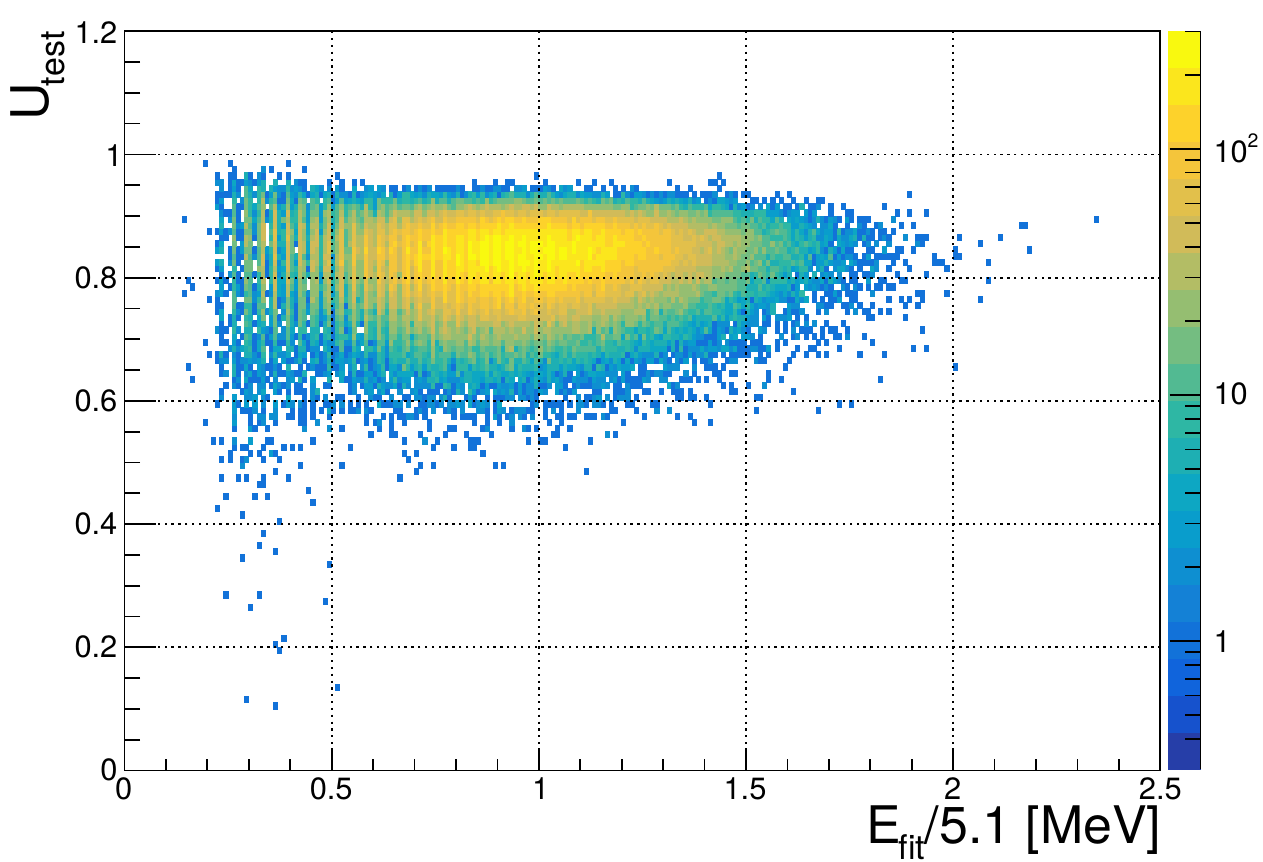
\includegraphics[width=7.5cm]{Utest_data_N16_107055.png}
			\end{minipage}
		}
		\caption{$^{16}$N central-run 107055, $U_{test}$ vs. $E_{fit}$/5.1 MeV.}
		\label{energyFOM_Utest}
	\end{figure}
	
	\item[$\bullet$] $G_{test}$: Fig.~\ref{energyFOM_Gtest} shows $G_{test}$ vs. energy biases. A cut of $0<G_{test}<1.9$ was suggested by the collaboration, which removes 0.01\% events for both MC and data.	
	
	\begin{figure}[!htb]
		\centering
		\subfigure[MC]{ 
			\begin{minipage}[t]{0.5\textwidth}
				\centering
				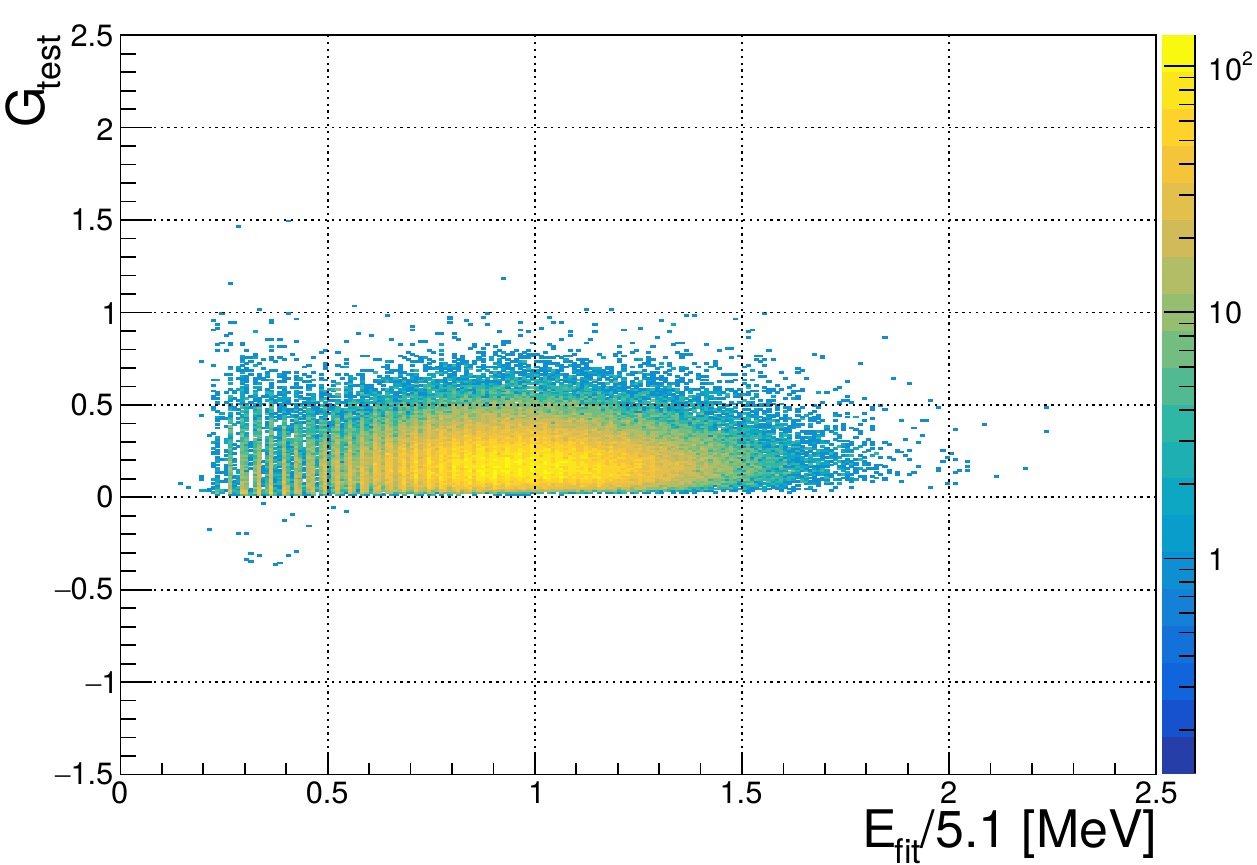
\includegraphics[width=7.5cm]{Gtest_MC_N16_107055.png}
			\end{minipage}
		}
		\subfigure[data]{ 
			\begin{minipage}[t]{0.4\textwidth}
				\centering
				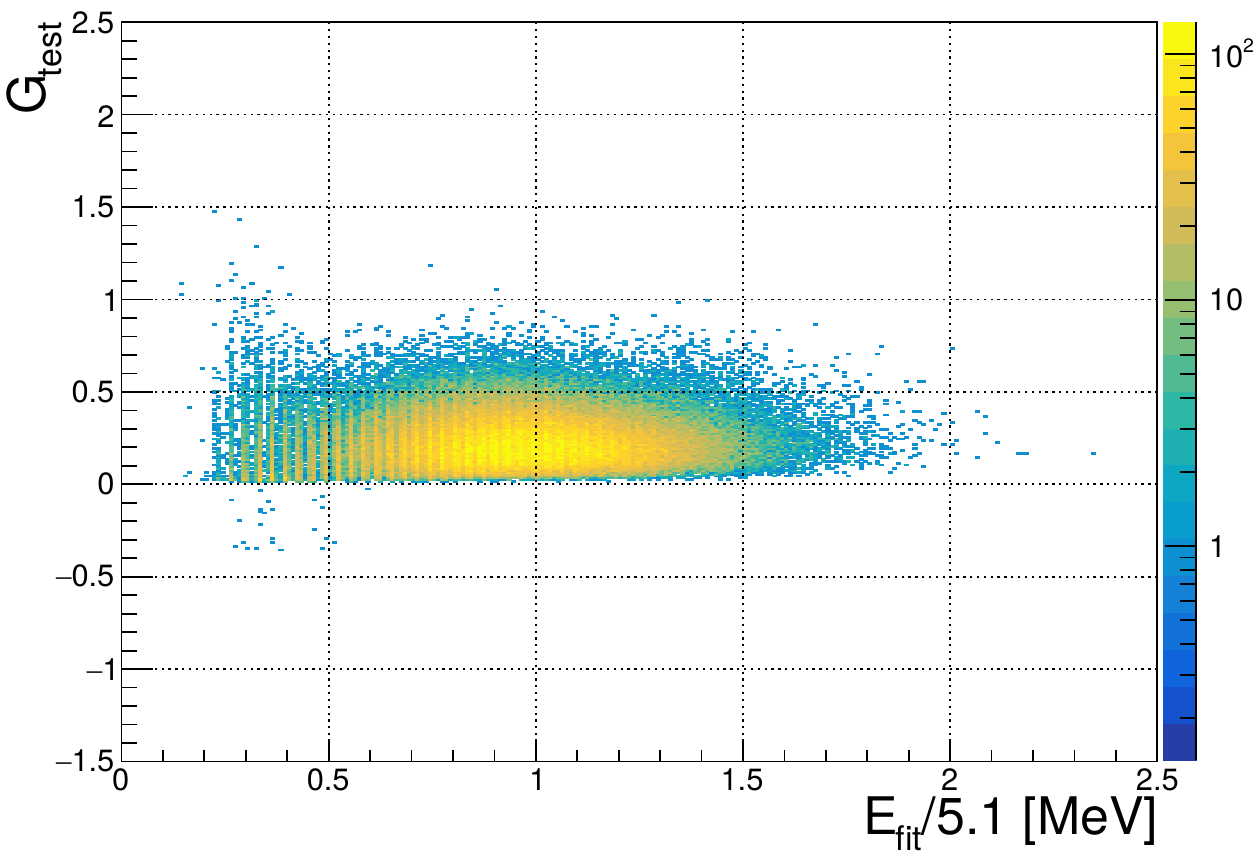
\includegraphics[width=7.5cm]{Gtest_data_N16_107055.png}
			\end{minipage}
		}
		\caption{$^{16}$N central-run 107055, $G_{test}$ vs. $E_{fit}$/5.1 MeV.}
		\label{energyFOM_Gtest}
	\end{figure}
	
	\item[$\bullet$]$Z_{factor}$:
	Fig.~\ref{energyFOM_Zfactor} shows $Z_{factor}$ vs. energy biases. A cut of $-11<Z_{factor}<1$ was suggested by the collaboration, which removes 0.13\% events for both MC and data.		
	\begin{figure}[!htb]
		\centering
		\subfigure[MC]{ 
			\begin{minipage}[t]{0.5\textwidth}
				\centering
				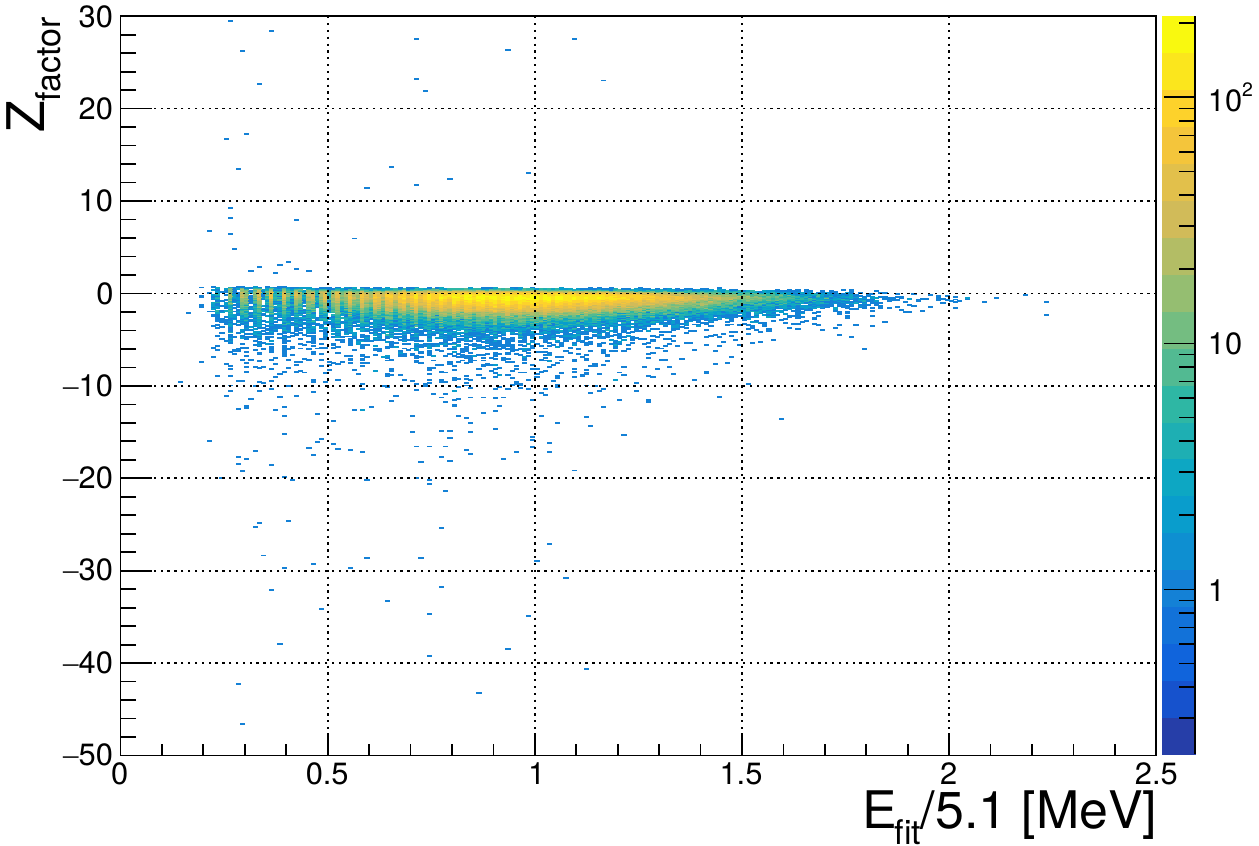
\includegraphics[width=7.5cm]{Zfactor_MC_N16_107055.png}
			\end{minipage}
		}
		\subfigure[data]{ 
			\begin{minipage}[t]{0.4\textwidth}
				\centering
				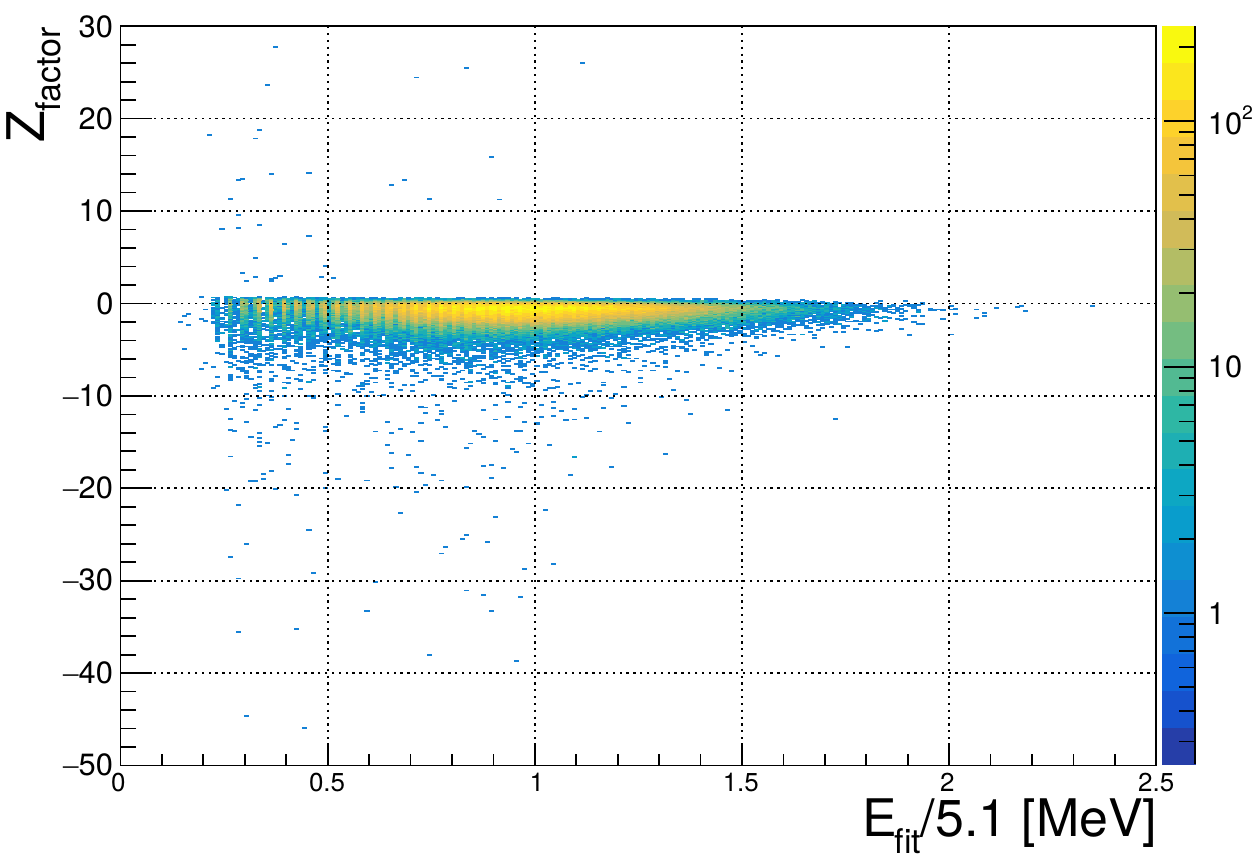
\includegraphics[width=7.5cm]{Zfactor_data_N16_107055.png}
			\end{minipage}
		}
		\caption{$^{16}$N central-run 107055, $Z_{factor}$ vs. $E_{fit}$/5.1 MeV.}
		\label{energyFOM_Zfactor}
	\end{figure}
	
	
\end{itemize}

All the cuts on the three energy FoM quantities removes 0.40\% events from MC and 0.37\% events from data. These cuts were also used in the water phase analysis which will be described in the next chapter.

\subsubsection{Eenrgy Resolution and Systematics}
The RSP energy reconstruction algorithm mentioned in Chapter 4 was applied on $^{16}$N MC simulations and data. 
The reconstructed energy of the $^{16}$N events are shown in Fig.~\ref{N16energy}. The results from the MC and the data are compared.
\begin{figure}[htbp]
	\centering
	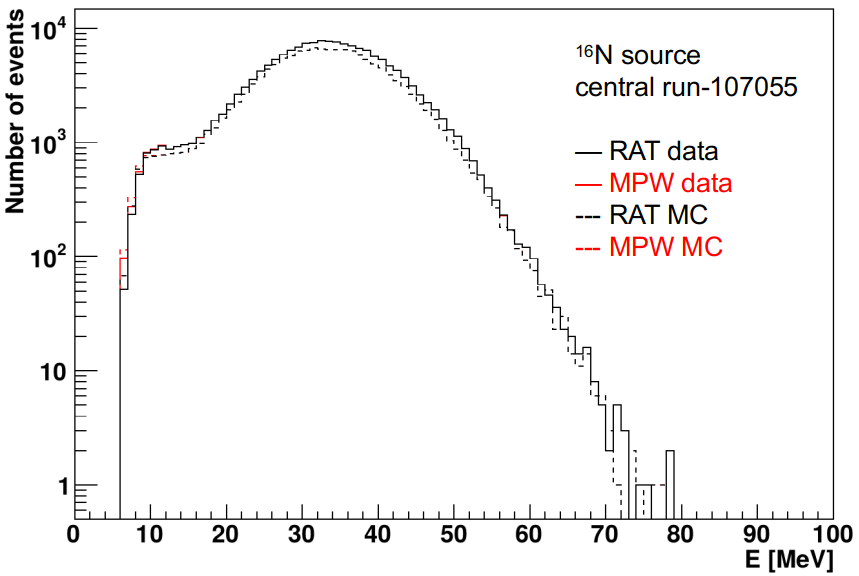
\includegraphics[width=10cm]{N16_nhits_107055.png}
	\caption{NHit spectrum for the $^{16}$N central run-107055. Dashed lines for the MC and solid lines for data; red for the MPW fitter results and black for the Rat results.}
	\label{N16nhits}
\end{figure}

\begin{figure}[htbp]
	\centering
	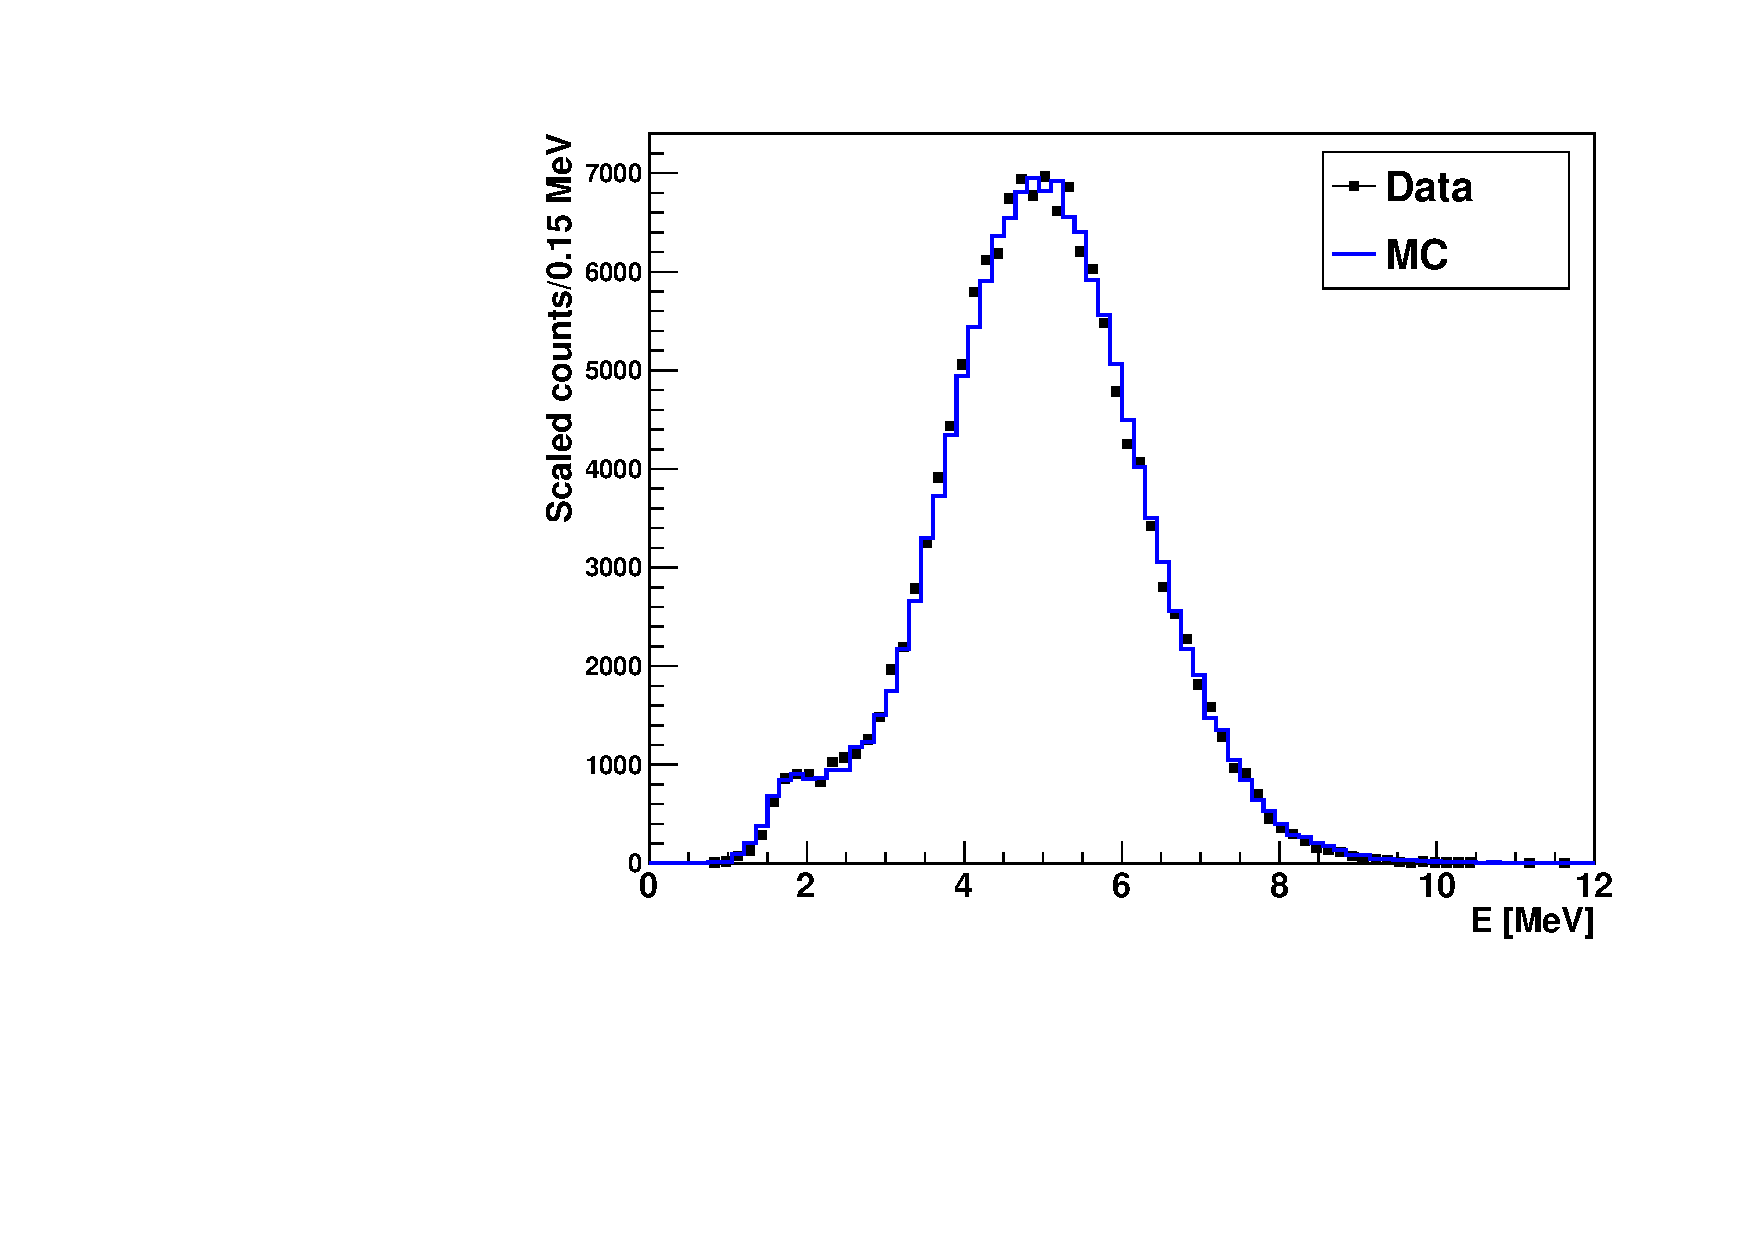
\includegraphics[width=8cm]{N16energyMPWcompare_106925.pdf}
	\caption{Reconstructed $^{16}$N energy spectrum for run-106925 ($\vec{X}_{source}=(-186.0,254.0,-4999.899)$ mm).}
	\label{N16_106925}
\end{figure}

\begin{figure}[htbp]
	\centering
	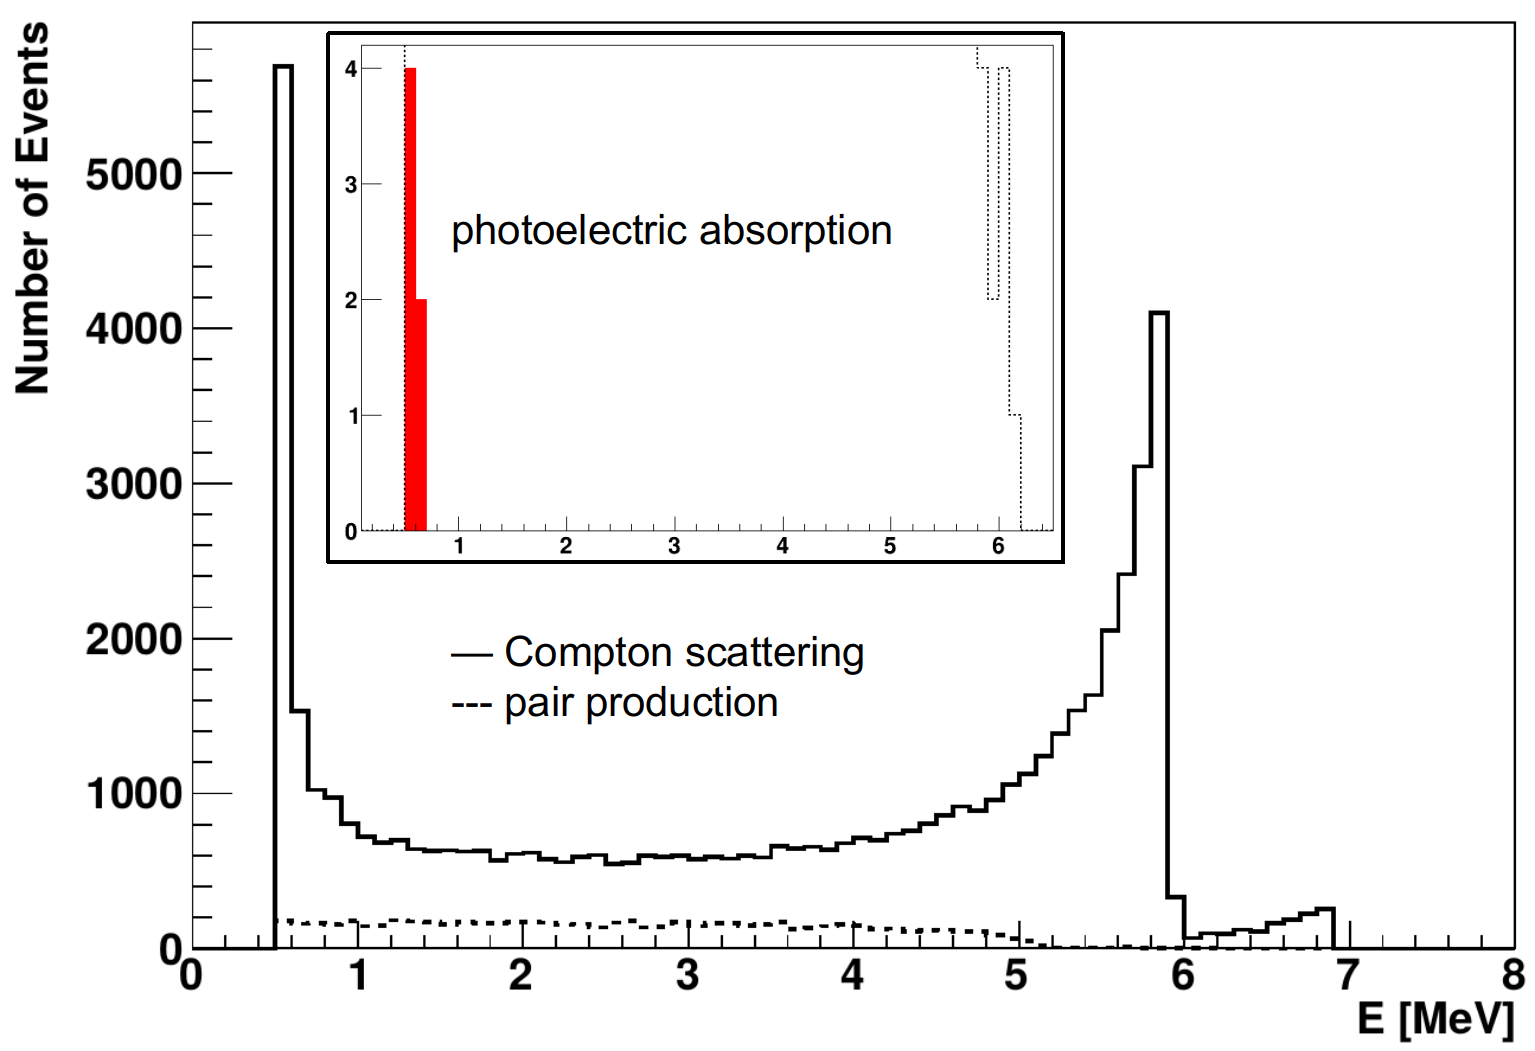
\includegraphics[width=12cm]{N16_MCenergySpectrum.png}
	\caption{Simulated energy spectrum for different processes, extracted from $10^5$ MC simulation events.}
	\label{N16nhitsSimu}
\end{figure}


The energy spectrum of the photons is converted into an apparent electron energy spectrum\cite{waterunidoc}.

By simulating mono-energetic electrons events with different energies,

A 2D map describes the relationship between the number of Cherenkov photons and electron energy is shown in Fig.~\ref{N16energyMap}.  

\begin{figure}[htbp]
	\centering
	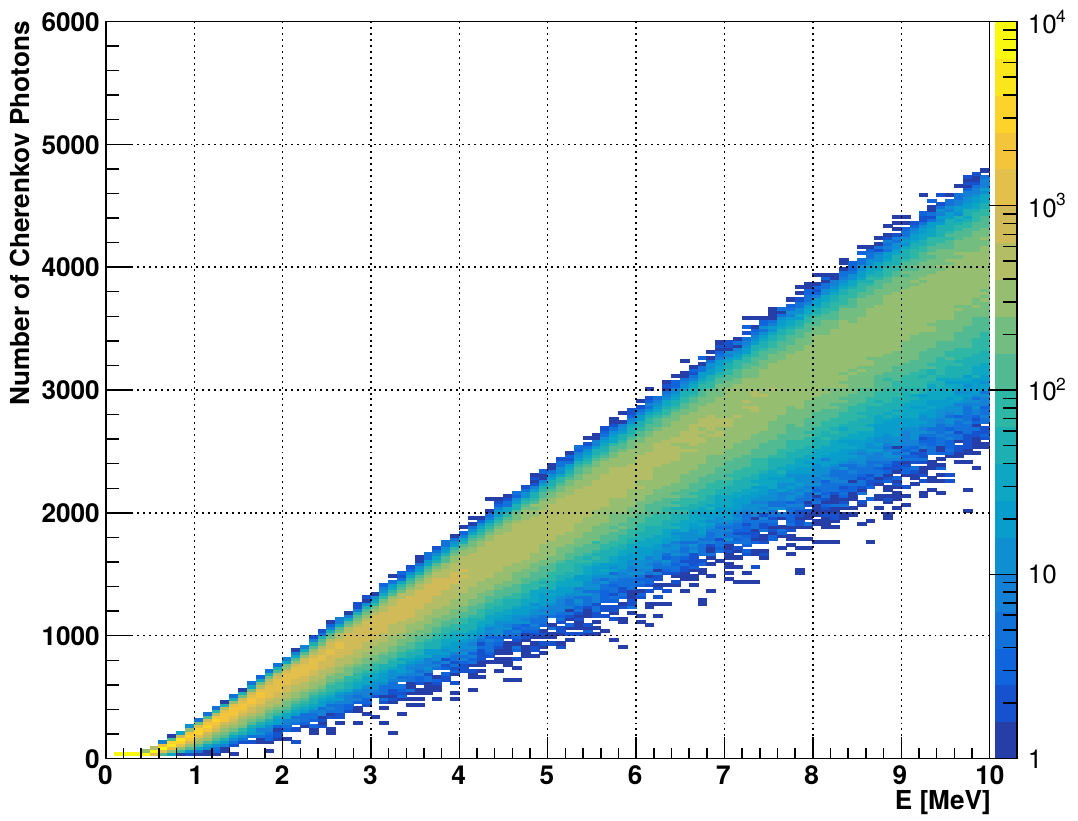
\includegraphics[width=10cm]{2dmap_EvsNphoton.png}
	\caption{Electron energy vs number of Cherenkov photons.}
	\label{N16energyMap}
\end{figure}

\begin{figure}[htbp]
	\centering
	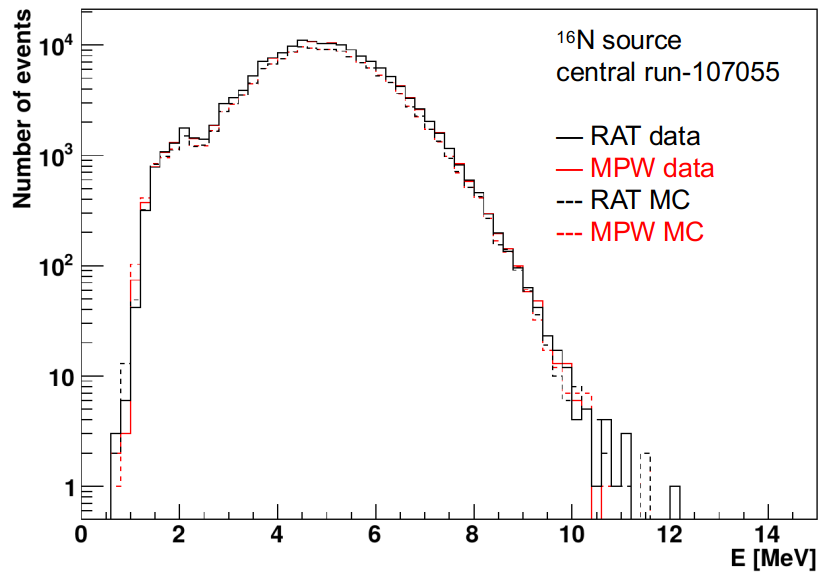
\includegraphics[width=10cm]{N16_reconE_107055.png}
	\caption{Reconstructed energy spectrum from the $^{16}$N central run-107055. Dashed lines for the MC and solid lines for data; red for the MPW fitter results and black for the Rat results.}
	\label{N16energy}
\end{figure}

\begin{figure}[htbp]
	\centering
	\subfigure[MPW data]{ 
		\begin{minipage}[t]{0.4\textwidth}
			\centering
			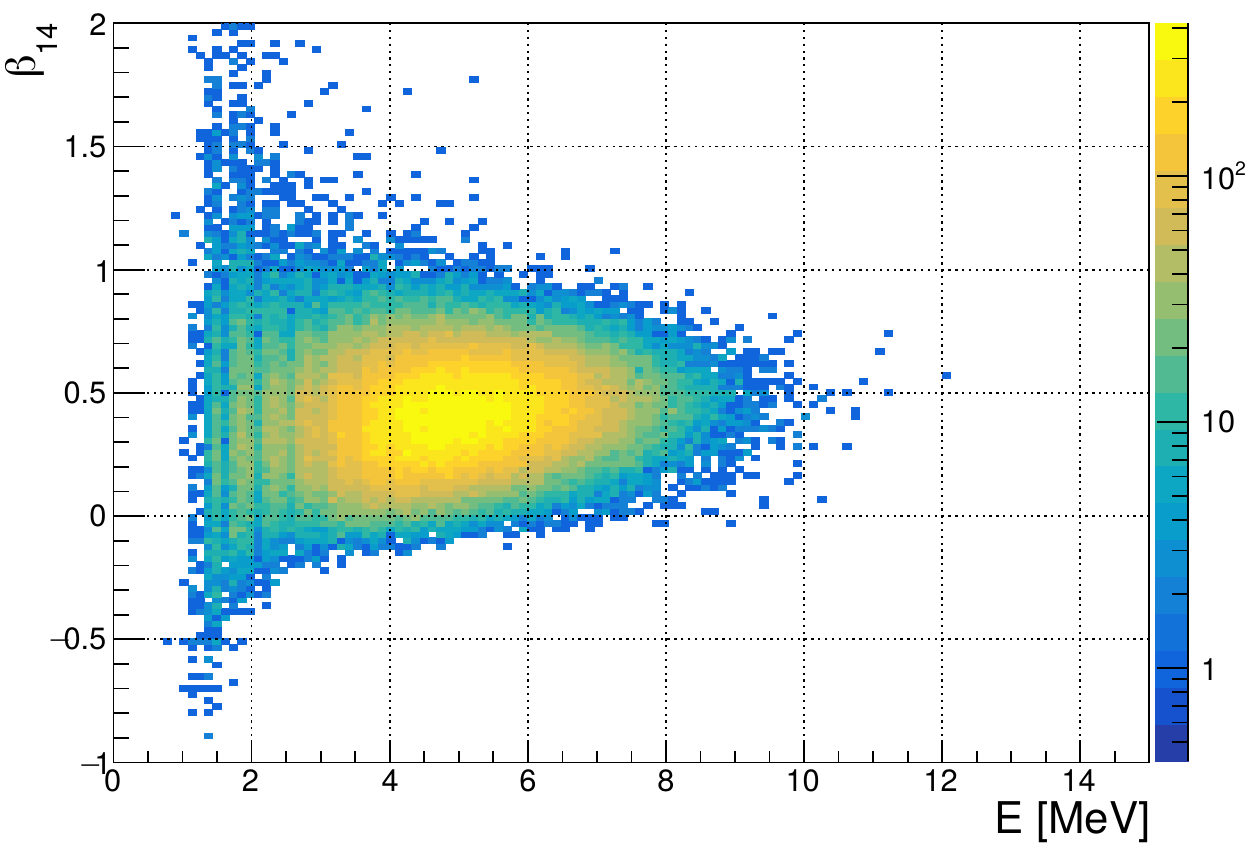
\includegraphics[width=6cm]{N16_MPW_data_EvsBeta14.png}
		\end{minipage}
	}
	\subfigure[MPW MC]{ 
		\begin{minipage}[b]{0.4\textwidth}
			\centering
			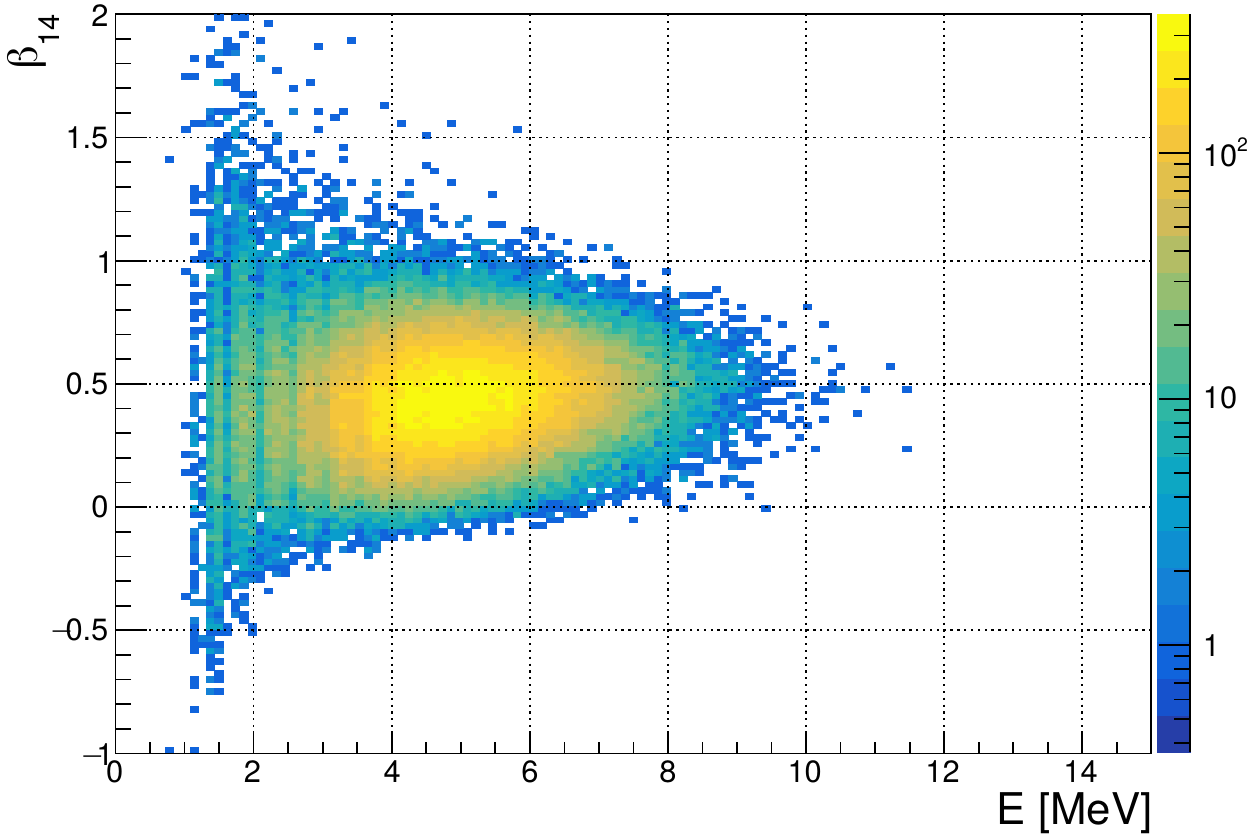
\includegraphics[width=6cm]{N16_MPW_mc_EvsBeta14.png}
		\end{minipage}
	}
	\subfigure[Rat data]{ 
		\begin{minipage}[t]{0.4\textwidth}
			\centering
			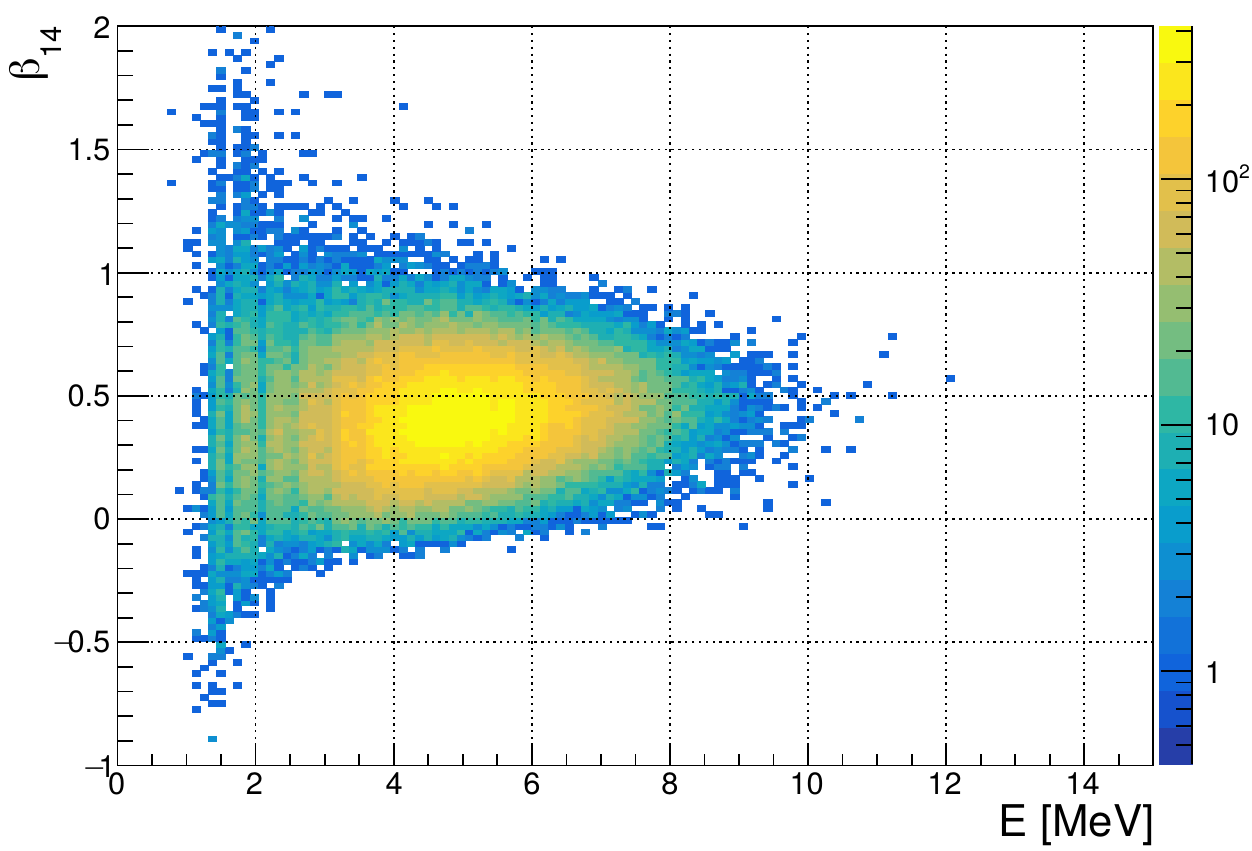
\includegraphics[width=6cm]{N16_rat_data_EvsBeta14.png}
		\end{minipage}
	}
	\subfigure[Rat MC]{ 
		\begin{minipage}[t]{0.4\textwidth}
			\centering
			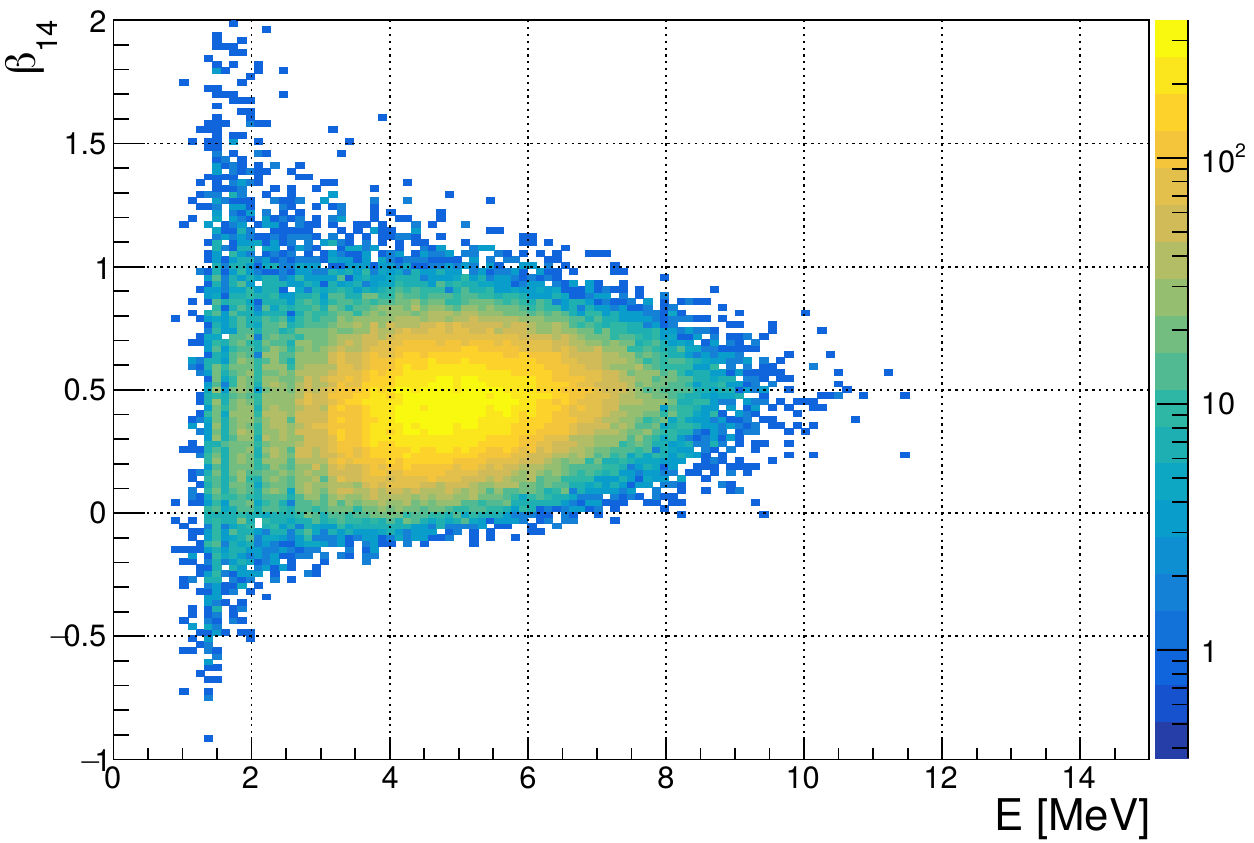
\includegraphics[width=6cm]{N16_rat_mc_EvsBeta14.png}
		\end{minipage}
	}
	\caption{Energy vs $\beta_{14}$ for the data and MC. Both the Rat and the MPW results are shown.}
	\label{EvsBeta14}
\end{figure}


\subsubsection{Energy Resolutions}

To obtain the energy reconstruction resolutions, the reconstructed energy spectrum $P(T_{eff})$ is fitted with the energy resolution function defined as\cite{waterunidoc}:

\begin{equation}
P(T_{eff})=N\int P_{source}(T_e)\frac{1}{\sqrt{2\pi}\sigma}\exp \{-\frac{[(1+\delta_E)T_{eff}-T_e]^2}{2\sigma^2}\},
\end{equation}

where the predicted apparent energy spectrum, $P_{source}(T_e)$, is convolved with a Gaussian resolution function. The $P_{source}(T_e)$ spectrum includes 

In the Gaussian function, $\sigma$ is the detector resolution and $\sigma = b\sqrt {T_{eff}}$.

Before fitting the reconstructed energy spectrum with the energy resolution function, a few cuts were applied on both the data and MC: the position FoM cut $scaleLogL>10$ and the energy FoM cuts: $0<G_{test}<1.9$, $U_{test}<0.95$ and $-11<Z_{factor}<1$ mentioned in the previous sections were used; the cuts of $NHit>5$, $ITR>0.55$ and $-0.12<\beta_{14}<0.95$ were used to remove instrumental backgrounds; a distance cut: $d(\vec{X}_{fit},\vec{X}_{src})>700~mm$ was suggested by \cite{leta,waterunidoc} to remove the shadow effects when the events are close to the source container; for the event reconstructed within the $700~mm$ distance, if its direction $\vec{u}_{fit}$ is within 45$^\circ$ of the vector from the source to its vertex, i.e., if $\sqrt2/2<\vec{u}_{true}\cdot \vec{u}_{fit}<1$, its energy will also be kept.

A default fit range of [3.5, 8.8]~MeV was suggested by \cite{waterunidoc} to remove poorly reconstructed events due to the trigger inefficiency.

Fig.~\ref{fittedEnergyResol} shows the reconstructed energy spectrum fitted with the energy resolution functions, for both the MC and data.
\begin{figure}
	\centering
	\subfigure[MC]{\includegraphics[width=60mm]{N16mc_energy_fitted_107055.pdf}}
	\subfigure[data]{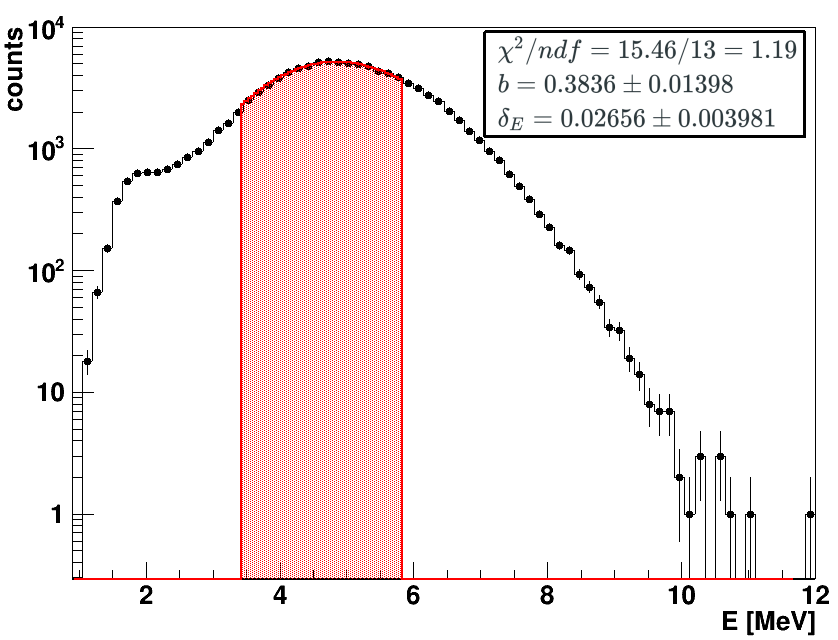
\includegraphics[width=60mm]{N16data_energy_fitted_107055.pdf}}
	\caption{Fitted energy resolution function (red) with the reconstructed energy of $^{16}$N central run-107055 MC (a) and data (b).}
	\label{fittedEnergyResol}
\end{figure}


\subsubsection{Energy Uncertainties}
$\Delta^2_\delta\equiv (\delta_{E,data}-\delta_{E,MC})^2+Error^2_{\delta,data}+Error^2_{\delta,MC}$

$\Delta^2_b\equiv (b_{E,data}-b_{E,MC})^2+Error^2_{b,data}+Error^2_{b,MC}$

$\bar{\Delta}=\sum_i^{N_{cells}}f_i\Delta_i$, where $\sum_i^{N_{cells}}f_i=1$
$f_i$: the fractional volume of cell $i$

$f_i = S_{cell}/S_{total} = (857*1000)/(\pi\cdot6000^2)$



$f_i = S_{cell}/S_{total} = (640*1000)/(12000 \cdot \sqrt{2*6000^2}$)


$\overline{\Delta_{\delta_E}}$

$\overline{\Delta_b}$

the uncertainties of the reconstructed energy scale and resolution.

Fig.~\ref{map_energyScale} and Fig.~\ref{map_energyResol} show the maps of the energy scale ($\Delta$) and the resolution parameter ($b$) respectively.

$570~mm\times 2000~mm$ cells of $z_{fit}\times \rho_{fit}$.

\begin{table}[ht]
	\centering
	\caption{Energy scales and resolutions.}
	\vspace{3mm}
	\label{table:energyScale}
	\begin{tabular*}{100mm}{c@{\extracolsep{\fill}}cc}
		\toprule
		& Data &  MC    \\
		\hline 
		b (MPW) & 0.006\%    &  $(1+0.006/100)\cdot x_{MC}$\\	
		$\delta_E$ (MPW) & -0.026 \%  & $(1-0.026/100)\cdot y_{MC}$\\
	%	\hline 
	%	b (Rat6.5.5) & 0.006\%    &  $(1+0.006/100)\cdot x_{MC}$\\	
	%	$\delta_E$ (Rat6.5.5) & -0.026 \%  & $(1-0.026/100)\cdot y_{MC}$\\
		\bottomrule
	\end{tabular*}
\end{table}

%\begin{figure}[!htb]\label{map_energyScale}
%	\centering
%	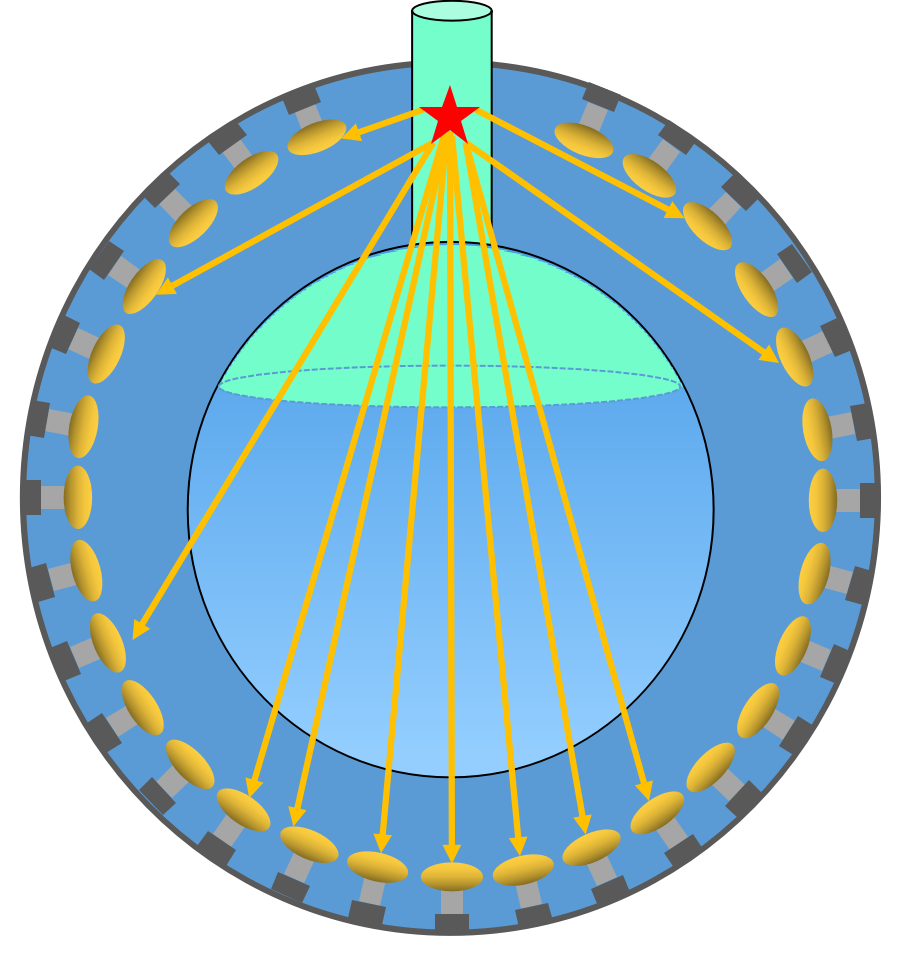
\includegraphics[width=5.5cm]{skyShine.png}
%	\caption{A map of relative energy scale $\delta_E$ across the detector.}
%
%\end{figure}
%
%\begin{figure}[!htb]\label{map_energyResol}
%	\centering
%	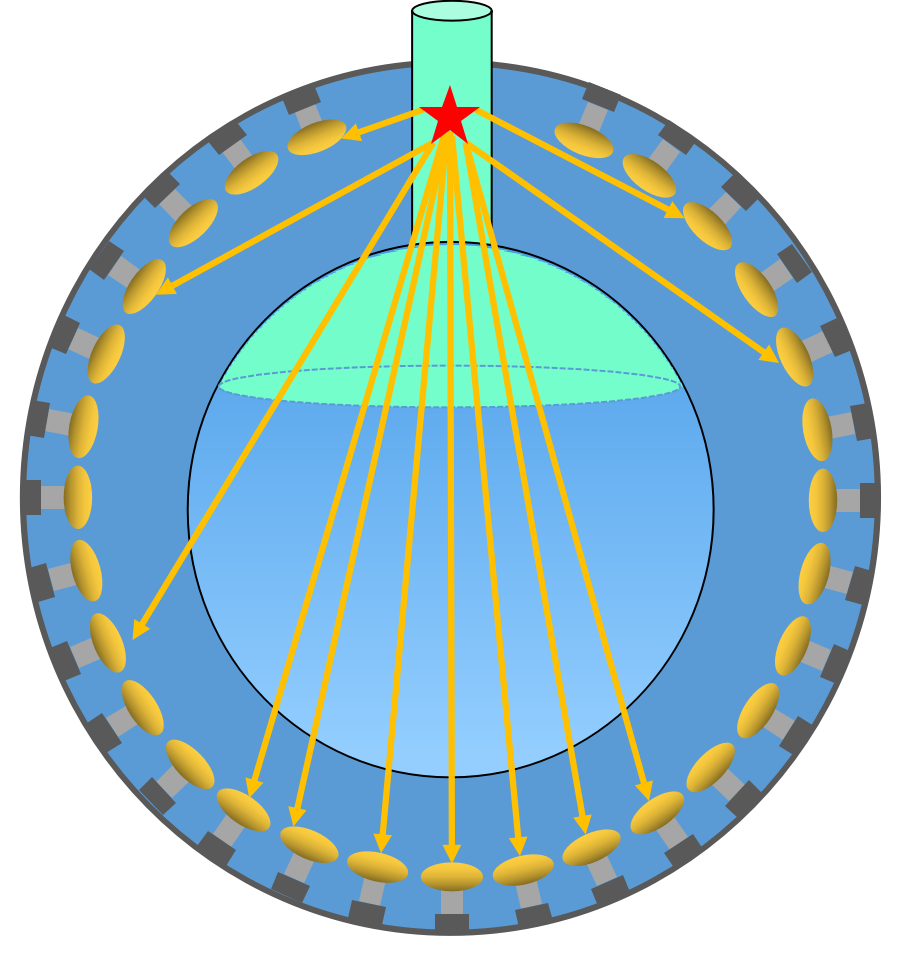
\includegraphics[width=5.5cm]{skyShine.png}
%	\caption{A map of relative energy scale $\delta_E$ across the detector.}
%\end{figure}

\section{Extracting \texorpdfstring{$\gamma$}{Lg}-rays from Neutron Capture}
The AmBe calibration source is used for the calibrations of the SNO+ neutron capture process.


\section{$^{16}$N Calibration in Partial-fill Phase}

During the August to October 2019, the PPO is added into the LAB when the water level was at 5100 mm (in PSUP coordinate). This is one of the stages of the partial-fill phase.

As mentioned in Chapter 3, the main purpose of the partial-fill phase is to identify the background level of the liquid scintillator. $^{16}$N and $AmBe$ calibration sources were also deployed in the external water to test the response of the detector. 

During the filling, the LAB was first filled into the AV to replace the water. PPO was later mixed with LAB and added into the AV. At some stage, the PPO concentration was kept at 0.53 g/L, which was lower than the nominal 2 g/L. At the lower PPO concentration, the liquid scintillator has a slower timing profile. This also brings an opportunity to extract the Cherenkov signals from the liquid scintillator with low PPO concentration.

\subsection{High Level Cuts: Sky-shine Classifier}
During the partial-fill phase, a Sky-shine classifier was suggested by Mark Chen and developed by Jeff Tseng to discriminate the noise events coming from the top of the detector, the so-called ``sky shine'' events, from other backgrounds events in the AV detection region\cite{skyshine}. These sky shine events are mostly the backgrounds from radioactive decays happening in the neck region. 

For an event happens in the neck region, it can trigger more PMTs in the bottom (or 
the lower hemisphere) of the PSUP sphere than in the higher hemisphere, as illustrated in Fig.~\ref{skyshine}. The classifier counts the number of the triggered PMTs with $z_{PMT}<-1000~mm$ (in PSUP coordinate) as $nSignal$ and the number of the ones with $-1000<z_{PMT}<8000~mm$ as $nSide$. The ratio $skyShine=nSide/nSignal$ is the output value of the classifier. Meanwhile, the classifier also saves the counts of the triggered neck PMTs ($nNeck$) as well as the triggered outward looking (OWL) PMTs in high z positions with $z_{OWL}>8000~mm$ ($nOWL$).

\begin{figure}[!htb]
	\centering
	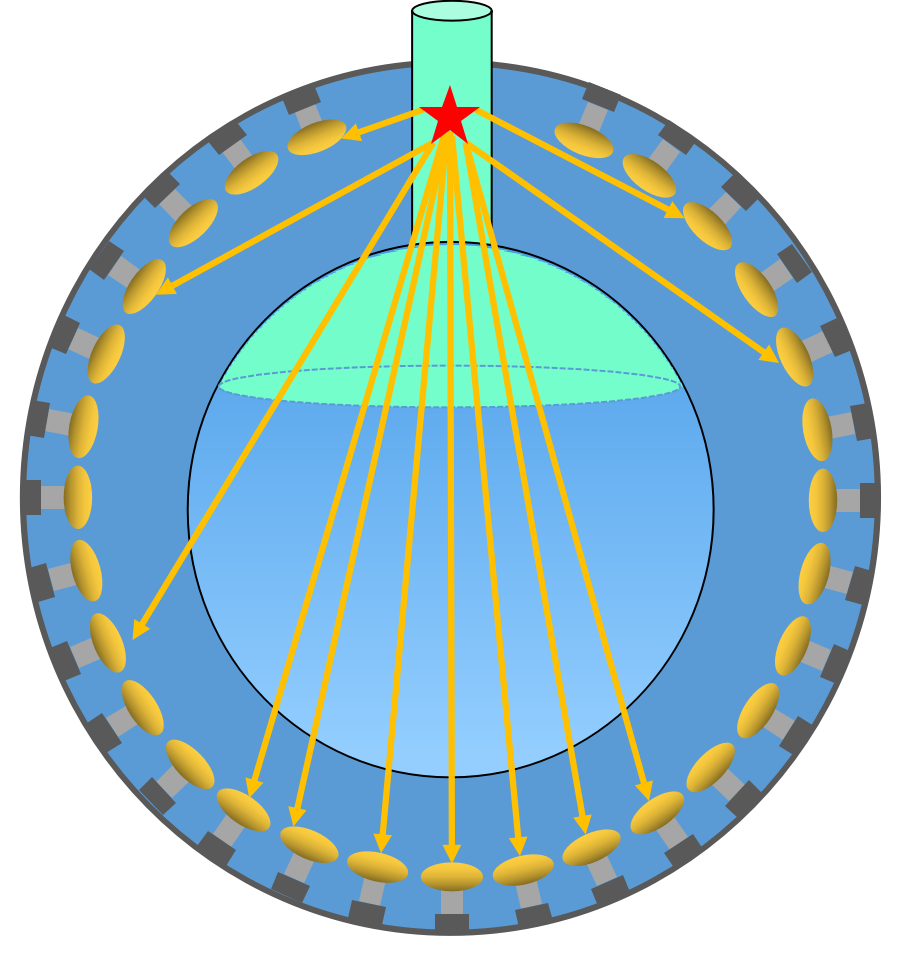
\includegraphics[width=5.5cm]{skyShine.png}
	\caption{ An illustration for the Sky-shine classifier, modified from \cite{skyshine}.}
	\label{skyshine}
\end{figure}

In the following, I studied the performance of the Sky-shine classifier and attempted to obtain an optimized cut on the value of $skyShine$ based on the MC simulations.

\subsubsection{Performance of the Sky-shine Classifier}
The MC simulations of the $^{208}$Tl decay events were produced in a partial-fill geometry with the water level set at 4435~mm (in AV coordination) and 2 g/L PPO concentration. The $^{208}$Tl decay events were distributed uniformly in the scintillator region. 4067 events of $^{208}$Tl decays were simulated (about 16 times the expected number of events per year based on the SNO+ background evaluations\cite{markchen_bkg}) and 3784 events were triggered. RAT version 6.16.9 was used. 

Fig.~\ref{Tl208simu} shows the positions of the simulated events and the fitted events. In the MC simulations, events are distributed in the AV as well as the whole region of the neck. Recall that the neck of the detector is 8-m tall, the MC simulated neck events from $z_{neck_bottom}=6108~mm$ up to about $z_{neck_top}=13000~mm$ in the PSUP coordinate. The valid reconstruction region is inside the PSUP sphere, thus only a small fraction of the neck events in the volume of the neck cylinder inside the PSUP sphere can be fitted or even be triggered.

\begin{figure}
	\centering
	\subfigure[MC positions ($z_{mc}$ vs. $\rho_{mc}$)]{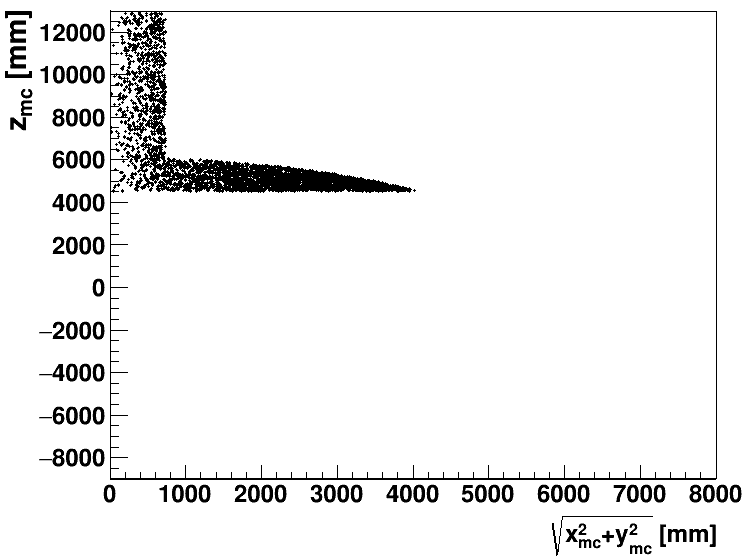
\includegraphics[width=60mm]{Tl208_p3_6169_mc.png}}
	\subfigure[Fitted positions ($z_{mc}$ vs. $\rho_{mc}$)]{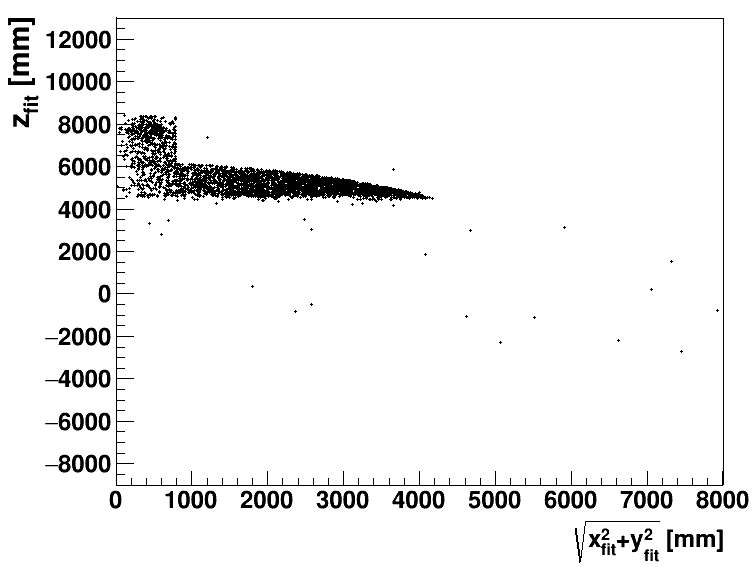
\includegraphics[width=60mm]{Tl208_p3_6169_fit.png}}
	\caption{MC (left) and fitted positions (right) of $^{208}$Tl simulations.}
	\label{Tl208simu}
\end{figure}

The plots shows events with small values of Sky-shine calculations can be tagged as neck events.
\begin{figure}
	\centering
	\subfigure[$x_{mc}$ vs. $skyShine$.]{\label{fig2:1a}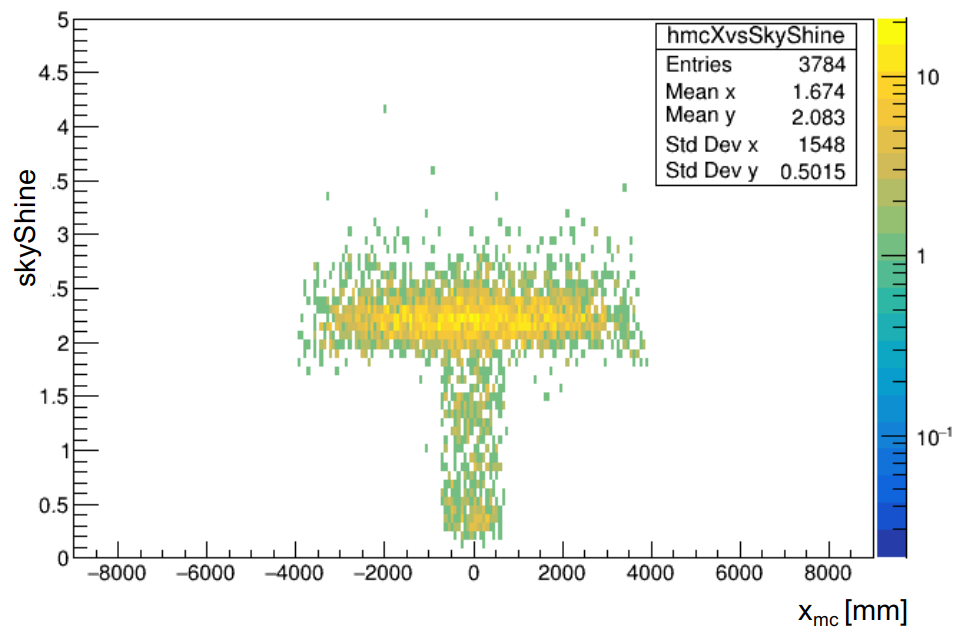
\includegraphics[width=60mm]{skyShineVsXmc.png}}
	\subfigure[$y_{mc}$ vs. $skyShine$.]{\label{fig2:1b}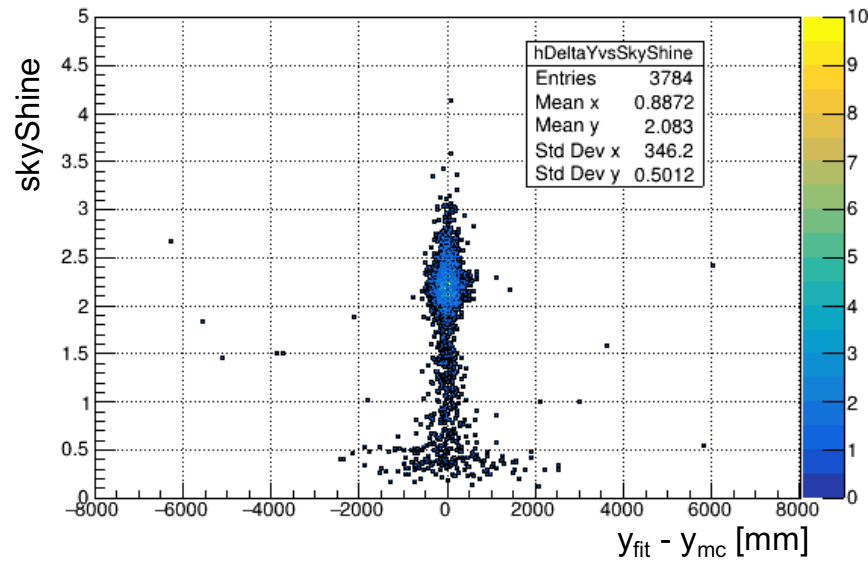
\includegraphics[width=60mm]{skyShineVsYmc.png}}
	\subfigure[$z_{mc}$ vs. $skyShine$.]{\label{fig2:1c}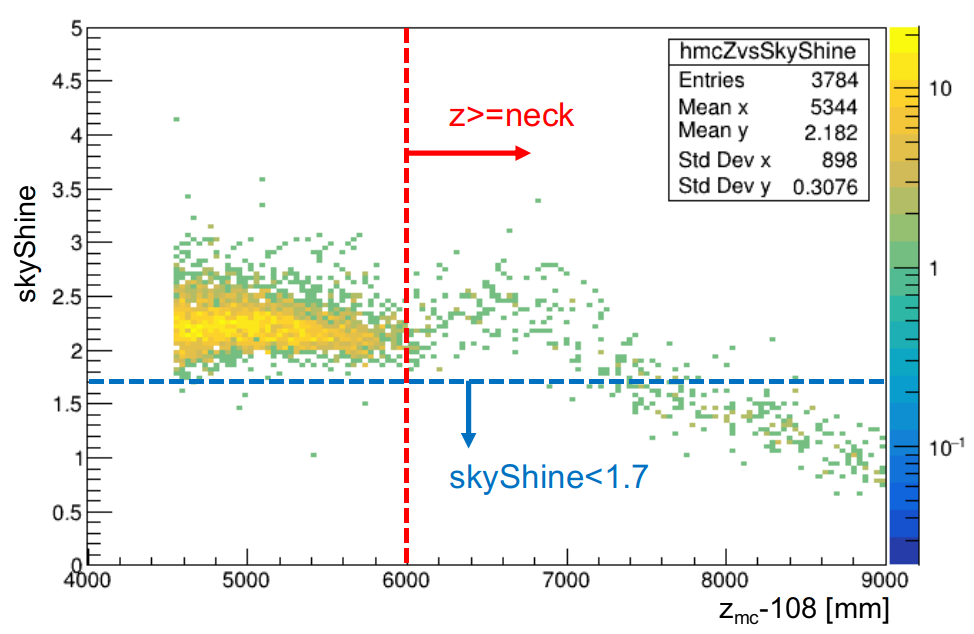
\includegraphics[width=60mm]{skyShineVsZmc.png}}
	\subfigure[$r_{mc}$ vs. $skyShine$.]{\label{fig2:1d}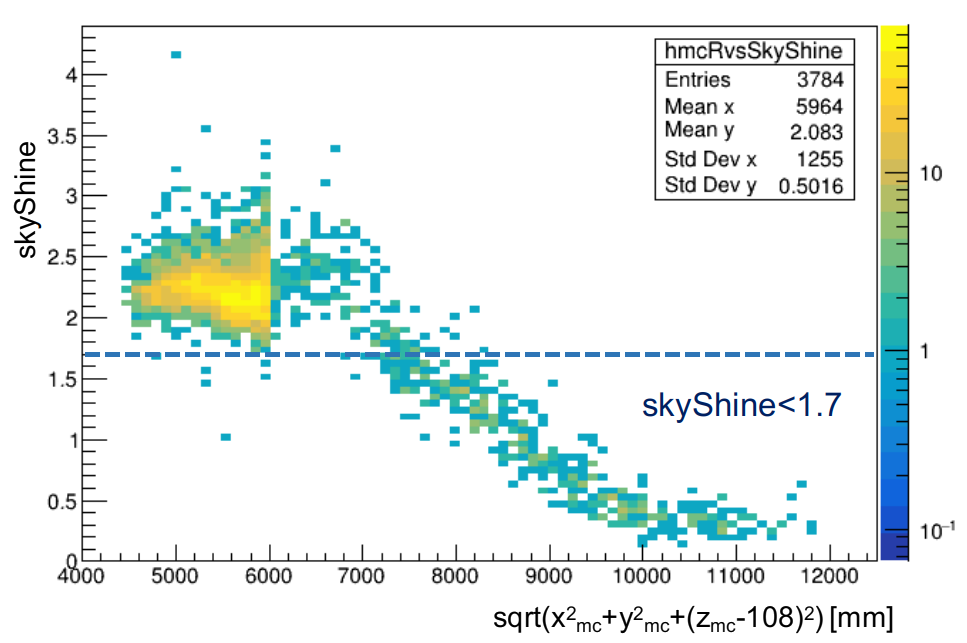
\includegraphics[width=60mm]{skyShineVsRmc.png}}
	\caption{MC positions vs. skyShine values for simulated $^{208}$Tl events.}
	\label{skyShineVsPos}
\end{figure}

\begin{figure}
	\centering
	\subfigure[$z_{mc}$ vs. $\rho_{mc}$, with $skyShine<1.7$.]{\label{fig2:2a}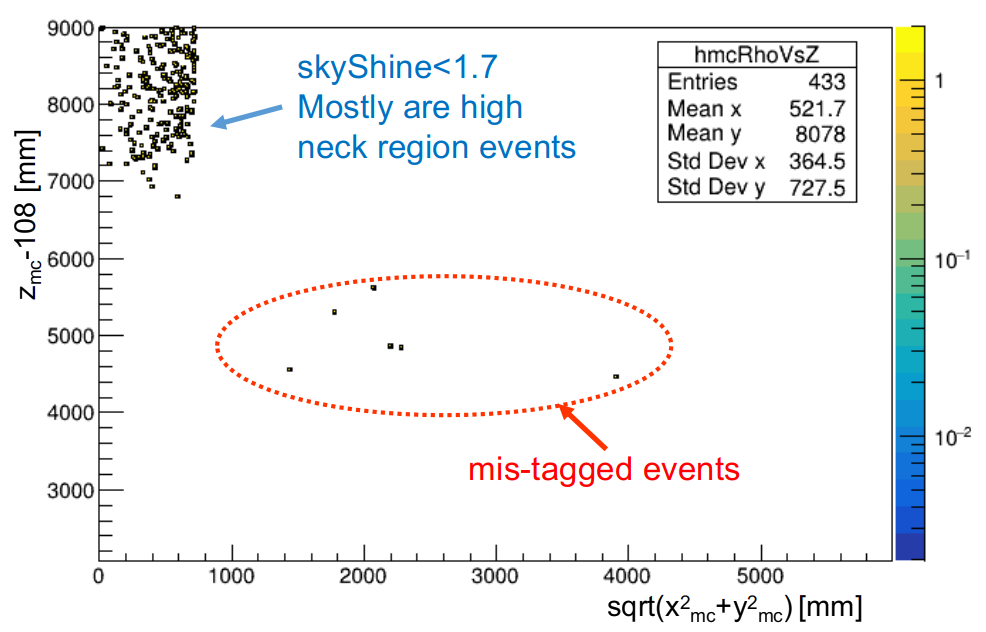
\includegraphics[width=60mm]{skyShineVsRho_mc.png}}
	\subfigure[$z_{mc}$ vs. $\rho_{mc}$, with $skyShine<1.5$.]{\label{fig2:2b}\includegraphics[width=60mm]{skyShineVsRho_mc1p5.png}}
	\caption{MC positions after Sky-shine cuts ($skyShine<1.7$ and $skyShine<1.5$) for simulated $^{208}$Tl events. It shows that most of the events with small $skyShine$ values are located in the neck region while very few events in the FV region can be mis-tagged.}\label{skySHineCutsVsMCpos}
\end{figure}

By checking the MC events positions (``true'' event positions),  for all the triggered events, 16.8\% of them are outside the AV. Apply skyShine>1.7 can remove 98.6\% of the events outside the AV (mostly in the neck) with a sacrifice of 0.2\% of the events inside the AV.

\subsubsection{Optimize the Sky-shine Cuts}

Since the Sky-shine classifier removes neck events (most of them are outside the PSUP) which are not properly fitted, a skyShine cut can reduce the fit biases and improve the fit resolution.

skyShine vs. fit biases (208Tl)

\begin{figure}
	\centering
	\subfigure[$x_{fit}-x_{mc}$ vs. $skyShine$.]{\label{fig2:3a}\includegraphics[width=50mm]{skyShineVsXbias.png}}
	\subfigure[$y_{fit}-y_{mc}$ vs. $skyShine$.]{\label{fig2:3b}\includegraphics[width=50mm]{skyShineVsYbias.png}}
	\subfigure[$z_{fit}-z_{mc}$ vs. $skyShine$.]{\label{fig2:3c}\includegraphics[width=50mm]{skyShineVsZbias.png}}
	\caption{Fit biases vs. skyShine values for simulated $^{208}$Tl events.}
	\label{skyShineVsFitBias}
\end{figure}

An improvement of $\sim 18$ mm in z resolution.

\begin{figure}
	\centering
	\subfigure[$x_{fit}-x_{mc}$ vs. $skyShine$.]{\label{fig2:4a}\includegraphics[width=50mm]{fitBiasX_noCuts_Tl208_partial.png}}
	\subfigure[$y_{fit}-y_{mc}$ vs. $skyShine$.]{\label{fig2:4b}\includegraphics[width=50mm]{fitBiasY_noCuts_Tl208_partial.png}}
	\subfigure[$z_{fit}-z_{mc}$ vs. $skyShine$.]{\label{fig2:4c}\includegraphics[width=50mm]{fitBiasZ_noCuts_Tl208_partial.png}}
	
	\subfigure[$x_{fit}-x_{mc}$ vs. $skyShine$.]{\label{fig2:4d}\includegraphics[width=50mm]{fitBiasX_skyShine1p7_Tl208_partial.png}}
	\subfigure[$y_{fit}-y_{mc}$ vs. $skyShine$.]{\label{fig2:4e}\includegraphics[width=50mm]{fitBiasY_skyShine1p7_Tl208_partial.png}}
	\subfigure[$z_{fit}-z_{mc}$ vs. $skyShine$.]{\label{fig2:4f}\includegraphics[width=50mm]{fitBiasZ_skyShine1p7_Tl208_partial.png}}
	
	\caption{Fit biases vs. skyShine values for simulated $^{208}$Tl events.}
	\label{skyShineVsFitResol}
\end{figure}

\begin{figure}
	\centering
	\includegraphics[width=60mm]{skyShineCuts.png}
	\caption{ Radial resolutions with different skyShine cuts.}
	\label{skySHineCutVsFitResol}.
\end{figure}

Apply different cuts of $skyShine$: $skyShine>1, 1.01, 2.0$, begins from 1.0 with a 0.01 step until 2.0.
Plot the x bias $x_{fit}-x_{mc}$ versus the $skyShine$ cut values.

Fit	a gaussian to $x_{fit} - x_{mc}$ and get $\sigma_x$,
Do the same thing to the $y_{fit} - y_{mc}$, $z_{fit} - z_{mc}$ and	obtain	$\sigma_x, \sigma_y, \sigma_z$
Fill a 1D histogram of Sky-shine cut and
$\Delta R= \sqrt{\sigma^2_x+\sigma^2_y+\sigma^2_z}$

Compare to the number of MC events inside the scintillator $\sqrt(x^2+y^2+(z-108)^2)<6005~mm \& z-108<6000~mm$, number of MC events/number fitted events after cut:
$skyShine>1.6$: 3149/3376
$skyShine>1.7$: 3149/3351
Can check with more productions/higher statistics.

\subsection{$^{16}$N Calibration in the Partial-fill Phase}

water level was at 5100 mm from the center of the AV (in AV coordination).
LAB with a PPO concentration of 0.53 g/L  

Effect of the water level.

The \isotope[16]{N} source was deployed in the external water region during the partial-fill phase.
run 251748 2019/09/19 and 

Source position was at $(-1120.8, 1041.4, 6172.5)~ mm$ for a 30-minute duration and at $(-1120.8. 1041.4, 6108.0)~mm$ for a 7-hour duration (separated into 7 runs).


\subsection{Extracting the Cherenkov Signals in Partial-fill Phase}

For an event happens in liquid scintillator, the number of Cherenkov photons it created is only $\sim 5\%$ 
of the total photon numbers, which is a very small fraction compared to the number of scintillation photons. This causes the directional Cherenkov signals are submerged in the isotropic lights.

Since the \isotope[16]{N} source provides high energy events around 6 MeV, 


a time cut window on the time residual was optimized for the searching based on MC.

simulations in pure scintillator phase.

\begin{figure}[!htb]
	\centering
	\includegraphics[width=8cm]{cherenkov_scint_variousE.png}
	\caption{Distributions of $\cos\theta_{PMT}$ after the prompt time cut for various $e^-$ energies simulations.}
	\label{cherenkov_variousE}
\end{figure}

\begin{figure}[htbp]
	\centering
	\subfigure[]{%PMT pattern before transformation.]{
		\begin{minipage}[t]{0.32\textwidth}
			\includegraphics[width=5.5cm]{partial0p5_6MeV_noRotate.pdf}
		\end{minipage}
	}   
	\subfigure[]{%PMT pattern before transformation, in sinusoidal map.]{ 
		\begin{minipage}[t]{0.32\textwidth}
			\centering
			\includegraphics[width=5.5cm]{partial0p5_sinu_6MeV_noRotate.pdf}
		\end{minipage}
	}
	\subfigure[]{%PMT pattern after transformation.]{ 
		\begin{minipage}[b]{0.32\textwidth}
			\centering
			\includegraphics[width=5.5cm]{partial0p5_6MeV_rotate.pdf}
		\end{minipage}
	}
	\subfigure[]{%PMT pattern after transformation, in sinusoidal map.]{ 
		\begin{minipage}[b]{0.32\textwidth}
			\centering
			\includegraphics[width=5.5cm]{partial0p5_sinu_6MeV_rotate.pdf}
		\end{minipage}
	}
	\caption{PMT hit patterns after the prompt time cut and NHit cut.}
	\label{6MeVisoPattern}
\end{figure}




In the case that $e^-$ are generated uniformly and isotropically in the detector, to enhance the 
Cherenkov ring pattern, a transformation is applied as following:

$\phi=\arccos(\hat{\vec{u}}_e\cdot\hat{\vec{u}}_{assume})$

$\vec{n}=\hat{\vec{u}}_e\times\hat{\vec{u}}_{assume}$
\[
R=\begin{bmatrix}
n^2_x(1-\cos\phi)+\cos\phi       &n_xn_y(1-\cos\phi)-n_z\sin\phi & n_xn_z(1-\cos\phi)+n_y\sin\phi \\
n_xn_y(1-\cos\phi)+n_z\sin\phi & n^2_y(1-\cos\phi)+\cos\phi & n_yn_z(1-\cos\phi)-n_x\sin\phi \\
n_xn_z(1-\cos\phi)-n_y\sin\phi & n_yn_z(1-\cos\phi)+n_x\sin\phi & n^2_z(1-\cos\phi)+\cos\phi
\end{bmatrix}
\]
$\vec{u'}_e=R\vec{u}_e$

$\vec{X'}_{evt}=R\vec{X}_{evt}$

Move $\vec{X'}_{evt}$ to the origin,

$\vec{X'}_{pmt}=R\vec{X}_{pmt}-\vec{X'}_{evt}$



Turning off the Cherenkov process in the Monte Carlo simulations.






Breit-Wigner function
\[
p(x) = \frac{c_0}{\pi}\frac{\frac{1}{2} \Gamma}{(x-m)^2 + (\frac{1}{2} \Gamma)^2}+c_1
\]

\begin{figure}[!htb]
	\centering
	\includegraphics[width=8cm]{partialN16.png}
	\caption{$\isotope[16]{N}$ source calibration in external water during the partial-fill phase.}
	\label{partialN16}
\end{figure}

\begin{figure}[!htb]
	\centering
	\includegraphics[width=8cm]{track_partial_N16.png}
	\caption{Simulated main track of 7.1 MeV $\gamma$ for one event from $\isotope[16]{N}$ source in the external water during the partial-fill phase.}	
	\label{track_partial_N16}
\end{figure}